%==============================================================================
% SUSTENTACIÓN — TRABAJO DE GRADO  (Julio 2026)
% Tratamiento numérico de la KHI bajo RRMHD
% Bryan Martinez Anzola  &  Sebastián Rodriguez Garcia
% Universidad Distrital Francisco José de Caldas
%
% Plantilla heredada de la presentación de avance (paleta Inferno).
% 28 láminas de cuerpo (~30 min) + referencias + 14 de respaldo (B1-B14).
% Plan detallado: PLAN_DIAPOSITIVAS.md
%
% COMPILACIÓN:
%   pdflatex main.tex && bibtex main && pdflatex main.tex && pdflatex main.tex
%
% Figuras: en figures/ (copiadas de monografia/figuras/, PDF vectorial).
%
% OJO (limitación del estilo de cajas): los títulos de tcolorbox
% [EQ=..., RES=..., HYP=..., WRN=...] NO pueden contener comas ni signos "=".
%==============================================================================
\documentclass[aspectratio=169,9pt]{beamer}

\usepackage[utf8]{inputenc}
\usepackage[T1]{fontenc}
\usepackage{amsmath,amssymb,mathtools}
\usepackage{physics}
\usepackage{graphicx}
\usepackage{booktabs,array}
\usepackage{xcolor}
\usepackage{tikz}
\usetikzlibrary{arrows.meta,positioning,calc,decorations.pathmorphing,shapes.geometric}
\usepackage{tcolorbox}
\tcbuselibrary{most,skins}
\usepackage[numbers,sort&compress]{natbib}
\newcommand{\parencite}{\citep}
\newcommand{\textcite}{\citep}
\usepackage{hyperref}

%------------------------------------------------------------------------------
% PALETA INFERNO  (sin alteraciones — identidad visual establecida)
%------------------------------------------------------------------------------
\definecolor{INF0}   {RGB}{0,   0,   4}
\definecolor{INF1}   {RGB}{20,  11,  52}
\definecolor{INF2}   {RGB}{58,   9,  99}
\definecolor{INF3}   {RGB}{114,  15,  83}
\definecolor{INF4}   {RGB}{164,  37,  45}
\definecolor{INF5}   {RGB}{208,  55,  27}
\definecolor{INF6}   {RGB}{237, 140,  11}
\definecolor{INF7}   {RGB}{252, 222,  76}
\definecolor{INF8}   {RGB}{252, 242, 171}
\definecolor{primary}{RGB}{20,  11,  52}
\definecolor{accent} {RGB}{242, 115,  32}
\definecolor{gold}   {RGB}{250, 172,  56}
\definecolor{soft}   {RGB}{252, 242, 171}
\definecolor{violet} {RGB}{87,  15, 109}
\definecolor{brick}  {RGB}{208,  55,  27}
\definecolor{bgwarm} {RGB}{248, 244, 240}

%------------------------------------------------------------------------------
% TEMA  (sin alteraciones)
%------------------------------------------------------------------------------
\usetheme{Madrid}
\usecolortheme[named=primary]{structure}
\setbeamercolor{palette primary}    {bg=primary,fg=soft}
\setbeamercolor{palette secondary}  {bg=violet, fg=soft}
\setbeamercolor{palette tertiary}   {bg=accent, fg=primary}
\setbeamercolor{palette quaternary} {bg=primary,fg=soft}
\setbeamercolor{titlelike}          {parent=palette primary}
\setbeamercolor{frametitle}         {bg=primary,fg=accent}
\setbeamercolor{block title}        {bg=primary,fg=gold}
\setbeamercolor{block body}         {bg=bgwarm, fg=INF0}
\setbeamercolor{block title alerted}{bg=brick,  fg=soft}
\setbeamercolor{block body alerted} {bg=brick!10,fg=INF0}
\setbeamercolor{block title example}{bg=violet, fg=soft}
\setbeamercolor{block body example} {bg=violet!8,fg=INF0}
\setbeamercolor{itemize item}       {fg=accent}
\setbeamercolor{itemize subitem}    {fg=brick}
\setbeamercolor{itemize subsubitem} {fg=INF3}
\setbeamercolor{enumerate item}     {fg=accent}
\setbeamercolor{footline}           {bg=primary,fg=soft}
\setbeamercolor{section in toc}     {fg=primary}

\usefonttheme{professionalfonts}
\setbeamerfont{title}     {size=\large, series=\bfseries}
\setbeamerfont{frametitle}{size=\small, series=\bfseries}
\setbeamerfont{block title}{size=\footnotesize,series=\bfseries}
\setbeamerfont{itemize/enumerate body}{size=\footnotesize}
\setbeamerfont{itemize/enumerate subbody}{size=\scriptsize}

\setbeamertemplate{itemize item}      {\color{accent}\small$\blacktriangleright$}
\setbeamertemplate{itemize subitem}   {\color{brick}\small$\triangleright$}
\setbeamertemplate{itemize subsubitem}{\color{INF3}\tiny$\bullet$}
\setbeamertemplate{navigation symbols}{}

\setbeamertemplate{footline}{%
  \leavevmode\hbox{%
    \begin{beamercolorbox}[wd=.28\paperwidth,ht=2.2ex,dp=1ex,leftskip=.2cm]{footline}%
      \color{gold}\scriptsize\insertshortauthor
    \end{beamercolorbox}%
    \begin{beamercolorbox}[wd=.44\paperwidth,ht=2.2ex,dp=1ex,center]{footline}%
      \color{soft}\scriptsize\insertshorttitle
    \end{beamercolorbox}%
    \begin{beamercolorbox}[wd=.28\paperwidth,ht=2.2ex,dp=1ex,rightskip=.2cm]{footline}%
      \color{gold}\scriptsize\hfill\insertframenumber/\inserttotalframenumber
    \end{beamercolorbox}%
  }%
}

\setbeamertemplate{frametitle}{%
  \nointerlineskip%
  \begin{beamercolorbox}[wd=\paperwidth,leftskip=0.4cm,rightskip=0.4cm,
                        sep=0pt,vmode]{frametitle}%
    \vskip2pt%
    {\usebeamerfont{frametitle}\insertframetitle\par}%
    \ifx\insertframesubtitle\empty\else%
      {\color{gold!70}\scriptsize\insertframesubtitle\par}%
    \fi%
    \vskip2pt%
  \end{beamercolorbox}%
  \begin{beamercolorbox}[wd=\paperwidth,ht=1.2pt]{palette tertiary}\end{beamercolorbox}%
}

%------------------------------------------------------------------------------
% TCOLORBOX  (sin alteraciones)
%------------------------------------------------------------------------------
\tcbset{
  EQ/.style={enhanced,colback=primary!5,colframe=accent,
    fonttitle=\bfseries\scriptsize\color{primary},title=#1,
    sharp corners,boxrule=0.8pt,left=3pt,right=3pt,top=2pt,bottom=2pt,
    attach boxed title to top left={yshift=-1.5mm,xshift=3mm},
    boxed title style={colback=accent,sharp corners,boxrule=0pt,
      left=2pt,right=2pt,top=1pt,bottom=1pt}},
  RES/.style={enhanced,colback=gold!10,colframe=gold,
    fonttitle=\bfseries\scriptsize\color{primary},title=#1,
    sharp corners,boxrule=0.8pt,left=3pt,right=3pt,top=2pt,bottom=2pt,
    attach boxed title to top left={yshift=-1.5mm,xshift=3mm},
    boxed title style={colback=gold,sharp corners,boxrule=0pt,
      left=2pt,right=2pt,top=1pt,bottom=1pt}},
  HYP/.style={enhanced,colback=violet!8,colframe=violet,
    fonttitle=\bfseries\scriptsize\color{soft},title=#1,
    sharp corners,boxrule=0.8pt,left=3pt,right=3pt,top=2pt,bottom=2pt,
    attach boxed title to top left={yshift=-1.5mm,xshift=3mm},
    boxed title style={colback=violet,sharp corners,boxrule=0pt,
      left=2pt,right=2pt,top=1pt,bottom=1pt}},
  WRN/.style={enhanced,colback=brick!8,colframe=brick,
    fonttitle=\bfseries\scriptsize\color{soft},title=#1,
    sharp corners,boxrule=0.8pt,left=3pt,right=3pt,top=2pt,bottom=2pt,
    attach boxed title to top left={yshift=-1.5mm,xshift=3mm},
    boxed title style={colback=brick,sharp corners,boxrule=0pt,
      left=2pt,right=2pt,top=1pt,bottom=1pt}}
}

%------------------------------------------------------------------------------
% METADATOS
%------------------------------------------------------------------------------
\title[Sustentaci\'on --- KHI en RRMHD]{%
  Tratamiento Num\'erico de la Inestabilidad de Kelvin--Helmholtz\\
  bajo el Marco de la Magnetohidrodin\'amica Relativista Resistiva}
\subtitle{Sustentaci\'on de Trabajo de Grado}
\author[Martinez \& Rodriguez]{%
  Bryan Martinez Anzola \and Sebasti\'an Rodriguez Garcia\\[2pt]
  {\scriptsize Director: Prof.\ Ph.D.\ Sergio Miranda-Aranguren}}
\institute[UD]{Universidad Distrital Francisco Jos\'e de Caldas}
\date{Bogot\'a, Julio 2026}

%==============================================================================
\begin{document}
%==============================================================================

%------------------------------------------------------------------------------
% S1 · PORTADA
%------------------------------------------------------------------------------
{
\setbeamertemplate{footline}{}\setbeamertemplate{headline}{}
\begin{frame}[plain]
\begin{tikzpicture}[remember picture,overlay]
  \node[at=(current page.center),inner sep=0]
    {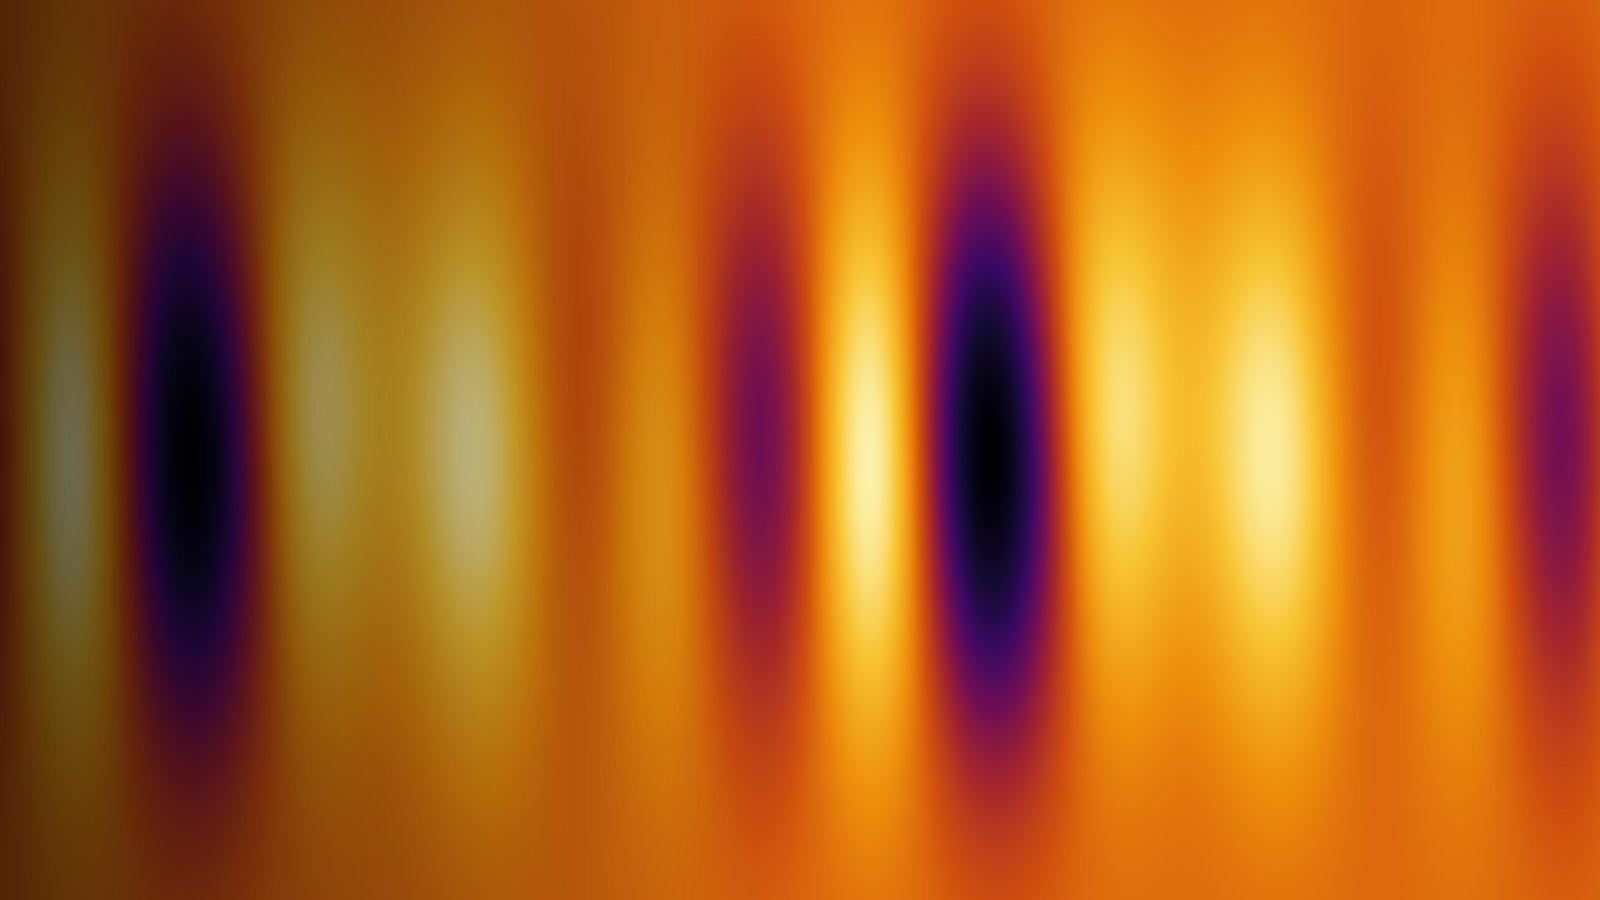
\includegraphics[width=\paperwidth,height=\paperheight,keepaspectratio=false]
     {figures/khi_simulation_bg.png}};
  \fill[primary,opacity=0.72]
    (current page.north west) rectangle
    ([xshift=0.62\paperwidth]current page.south west);
  \fill[primary,opacity=0.35]
    ([xshift=0.62\paperwidth]current page.north west) rectangle
    (current page.south east);
  \fill[accent]
    ([yshift=-0.225\paperheight]current page.north west)
    rectangle ([yshift=-0.270\paperheight]current page.north east);
  \shade[top color=accent,bottom color=gold]
    ([xshift=0.038\paperwidth]current page.south west)
    rectangle
    ([xshift=0.052\paperwidth,yshift=0.75\paperheight]current page.south west);
  \node[anchor=south east,inner sep=0]
    at ([xshift=-0.035\paperwidth,yshift=0.05\paperheight]current page.south east)
    {
\includegraphics[width=0.22\paperwidth]{figures/Logo_Escudo_invertido.png}};
\end{tikzpicture}

\begin{columns}[T]
\begin{column}{0.04\textwidth}\end{column}
\begin{column}{0.60\textwidth}
  \vspace{0.55cm}
  {\color{soft}\normalsize Tratamiento Num\'erico de la}\\[2pt]
  {\color{white}\Large\bfseries Inestabilidad de Kelvin--Helmholtz}\\[2pt]
  {\color{soft}\normalsize bajo el Marco de la}\\[1pt]
  {\color{gold}\large\bfseries Magnetohidrodin\'amica Relativista Resistiva}\\[4pt]
  {\color{accent}\rule{0.96\linewidth}{1.5pt}}\\[4pt]
  {\color{INF8}\scriptsize\itshape Sustentaci\'on de Trabajo de Grado}
  \vspace{0.28cm}\\
  {\color{gold}\scriptsize\bfseries Autores:}\\[1pt]
  {\color{INF8}\scriptsize Bryan Martinez Anzola
    $\;\cdot\;$ Sebasti\'an Rodriguez Garcia}\\[3pt]
  {\color{gold}\scriptsize\bfseries Director:}\\[1pt]
  {\color{INF8}\scriptsize Prof.\ Ph.D.\ Sergio Miranda-Aranguren}
  \vspace{0.22cm}\\
  {\color{gold}\scriptsize\bfseries Universidad Distrital Francisco Jos\'e de Caldas}\\
  {\color{INF8!70}\tiny Facultad de Ciencias Matem\'aticas y Naturales
    $\cdot$ Programa Acad\'emico de F\'isica}\\[2pt]
  {\color{INF8!60}\tiny Bogot\'a, Julio de 2026}
\end{column}
\begin{column}{0.36\textwidth}
  \vspace{0.3cm}
  \begin{center}
    {\color{INF8!50}\tiny c\'odigo \texttt{Cueva} --- RRMHD 2D}
  \end{center}
\end{column}
\end{columns}
\end{frame}
}

%------------------------------------------------------------------------------
% S2 · HOJA DE RUTA
%------------------------------------------------------------------------------
\begin{frame}{Estructura de la Presentaci\'on}
\begin{columns}[T]
\begin{column}{0.52\textwidth}
  \tableofcontents
\end{column}
\begin{column}{0.44\textwidth}
  \begin{tcolorbox}[RES={Objetivos espec\'ificos del trabajo}]
    \scriptsize
    \begin{enumerate}\setlength\itemsep{3pt}
      \item Cuantificar el efecto de la resistividad sobre la
            \textbf{tasa de crecimiento lineal} $\gamma_{\rm KHI}(\sigma)$.
      \item Analizar su efecto en la formaci\'on de
            \textbf{estructuras secundarias} (v\'ortices, l\'aminas de corriente).
      \item Evaluar el impacto de la difusi\'on magn\'etica sobre las
            \textbf{variables electromagn\'eticas globales}
            (corriente, energ\'ia magn\'etica, disipaci\'on).
      \item Evaluar c\'omo la \textbf{intensidad y orientaci\'on} del campo
            magn\'etico externo modifican la evoluci\'on de la inestabilidad.
    \end{enumerate}
  \end{tcolorbox}
  \vspace{0.15cm}
  {\scriptsize\color{primary}\textbf{Herramienta:} c\'odigo \texttt{Cueva}
   \citep{miranda-aranguren-2014,miranda-aranguren-2018} ---
   RRMHD en volumenes finitos, 2D.\\
   \textbf{Datos:} $44$ simulaciones (barrido en $\sigma$)
   $+$ $18$ configuraciones magn\'eticas.}
\end{column}
\end{columns}
\end{frame}

%==============================================================================
\section{Motivaci\'on y fenomenolog\'ia}
%==============================================================================

%------------------------------------------------------------------------------
% S3 · LA KHI SIN ECUACIONES
%------------------------------------------------------------------------------
\begin{frame}{El Fen\'omeno: la KHI en el Universo Relativista}
\framesubtitle{Qu\'e es, d\'onde vive y por qu\'e importa}
\begin{columns}[T]
\begin{column}{0.50\textwidth}
  \begin{block}{El mecanismo f\'isico (sin f\'ormulas)}
    \scriptsize
    \begin{itemize}\setlength\itemsep{2pt}
      \item Dos flujos en contacto con \textbf{velocidades distintas}
            $\Rightarrow$ capa de cizalla: un reservorio de energ\'ia libre.
      \item Una ondulaci\'on de la interfaz acelera el flujo sobre las crestas
            y lo frena en los valles $\Rightarrow$ por \textbf{Bernoulli},
            gradientes de presi\'on que ejercen un \textbf{torque} sobre la interfaz.
      \item El torque amplifica la ondulaci\'on $\Rightarrow$
            \textbf{crecimiento exponencial} (fase lineal) $\Rightarrow$
            enrollamiento en \textbf{v\'ortices} (fase no lineal).
    \end{itemize}
  \end{block}
  \begin{block}{Rol astrof\'isico}
    \scriptsize
    \begin{itemize}\setlength\itemsep{2pt}
      \item Fronteras de \textbf{chorros relativistas} de AGN y GRBs,
            vientos magnetizados, eyecciones de objetos compactos.
      \item Gobierna \textbf{mezcla y frenado} (\textit{entrainment}):
            morfolog\'ia FRI vs.\ FRII \citep{osmanov-2008}.
      \item Act\'ua como \textbf{d\'inamo}: los v\'ortices estiran las l\'ineas
            de campo y amplifican $B$ \citep{pimentel-2019}.
    \end{itemize}
  \end{block}
\end{column}
\begin{column}{0.46\textwidth}
  \begin{center}
    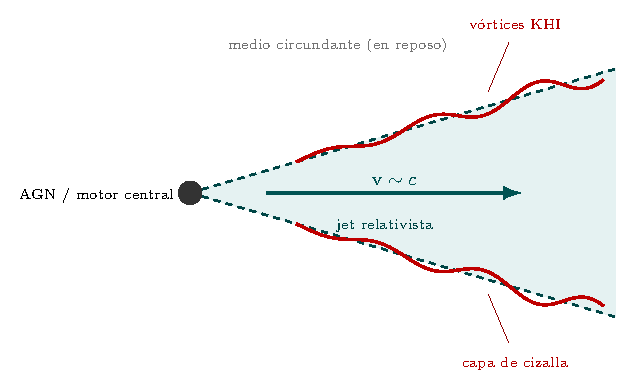
\includegraphics[width=\linewidth]{figures/contexto_jet.pdf}\\[2pt]
    {\tiny\color{INF3} Capa de cizalla en la frontera de un chorro de AGN:
     el contraste $\mathbf{v}\sim c$ / medio en reposo es
     inherentemente inestable frente a la KHI.}
  \end{center}
\end{column}
\end{columns}
\end{frame}

%------------------------------------------------------------------------------
% S4 · POR QUÉ RESISTIVA
%------------------------------------------------------------------------------
\begin{frame}{Por Qu\'e Resistiva: los L\'imites del Congelamiento Ideal}
\framesubtitle{De la RMHD ideal a la RRMHD}
\begin{columns}[T]
\begin{column}{0.48\textwidth}
  \begin{tcolorbox}[EQ={Inducci\'on: advecci\'on vs.\ difusi\'on}]
    \scriptsize
    \[
      \partial_t\mathbf{B}
      =\underbrace{\nabla\times(\mathbf{v}\times\mathbf{B})}_{\text{advecci\'on}}
      +\underbrace{\eta\,\nabla^2\mathbf{B}}_{\text{difusi\'on},\ \eta=1/\sigma}
    \]
    $\sigma\to\infty$: flujo magn\'etico \textbf{congelado} al fluido
    (teorema de Alfv\'en) $\Rightarrow$ la topolog\'ia de $\mathbf B$
    \emph{no puede} cambiar: la reconexi\'on est\'a prohibida.
  \end{tcolorbox}
  \vspace{0.12cm}
  \begin{tcolorbox}[WRN={El problema de la MHD ideal num\'erica}]
    \scriptsize
    Cuando un c\'odigo \emph{ideal} muestra reconexi\'on, esta proviene del
    \textbf{error de truncamiento} (``resistividad num\'erica''):
    un proceso incontrolado que depende de la malla, no de la f\'isica
    \citep{komissarov-2007}.
  \end{tcolorbox}
\end{column}
\begin{column}{0.48\textwidth}
  \begin{tcolorbox}[RES={Lo que habilita la resistividad f\'isica}]
    \scriptsize
    \begin{itemize}\setlength\itemsep{2pt}
      \item Reconexi\'on \textbf{natural, predictiva y f\'isica} en las
            l\'aminas de corriente ($\mathbf J=\nabla\times\mathbf B$ intensa).
      \item Calentamiento \'ohmico: conversi\'on irreversible
            $E_{\rm mag}\!\to\!$ calor.
      \item Escenarios donde es imprescindible: llamaradas de AGN/GRBs,
            magnetosferas de p\'ulsares, zonas turbulentas
            \citep{palenzuela-2009,miranda-aranguren-2018}.
    \end{itemize}
  \end{tcolorbox}
  \vspace{0.12cm}
  \begin{block}{La pregunta de esta tesis}
    \scriptsize
    ?`\textbf{C\'omo gobiernan la conductividad finita $\sigma$ y la geometr\'ia
    del campo $\mathbf B$} el crecimiento, la morfolog\'ia y el balance
    energ\'etico de la KHI relativista?
  \end{block}
\end{column}
\end{columns}
\end{frame}

%------------------------------------------------------------------------------
% S5 · OBJETIVOS Y DISEÑO EXPERIMENTAL
%------------------------------------------------------------------------------
\begin{frame}{Dise\~no del Experimento Num\'erico: Dos Campa\~nas}
\framesubtitle{Un solo montaje base --- dos ejes de la f\'isica no ideal}
\begin{columns}[T]
\begin{column}{0.48\textwidth}
  \begin{tcolorbox}[EQ={Campa\~na 1 --- Conductividad (objetivos 1--3)}]
    \scriptsize
    \[
      \sigma\in\{100,\,300,\,\ldots,\,10\,500\}\qquad(N=44)
    \]
    Todo lo dem\'as fijo $\Rightarrow$ se a\'isla el efecto de la
    difusividad magn\'etica $\eta=1/\sigma$ sobre:
    \begin{itemize}\setlength\itemsep{1pt}
      \item la tasa lineal $\gamma_{\rm KHI}(\sigma)$,
      \item la fenomenolog\'ia no lineal ($\Omega_{zp}^{\max}$, $t_{\rm peak}$),
      \item los diagn\'osticos electromagn\'eticos globales.
    \end{itemize}
  \end{tcolorbox}
\end{column}
\begin{column}{0.48\textwidth}
  \begin{tcolorbox}[HYP={Campa\~na 2 --- Campo magn\'etico (objetivo 4)}]
    \scriptsize
    Conductividad \textbf{fija} en dos reg\'imenes
    ($\sigma=6000$ y $\sigma=10^4$); se var\'ia $\mathbf B$:
    \begin{itemize}\setlength\itemsep{1pt}
      \item \textbf{A --- intensidad}: $B_0=1.0,\,1.5,\,2.0$
            (orientaci\'on Mizuno fija);
      \item \textbf{B --- orientaci\'on $y$--$z$}: rotaci\'on del campo gu\'ia
            hacia $\hat y\parallel\mathbf k$ (activa la \textbf{tensi\'on});
      \item \textbf{C --- orientaci\'on $x$--$z$}: $B_y=0$,
            $\mathbf k\cdot\mathbf B=0$ (\textbf{sin} tensi\'on).
    \end{itemize}
  \end{tcolorbox}
\end{column}
\end{columns}
\vspace{0.15cm}
\begin{center}
  
\includegraphics[width=0.32\textwidth]{figures/campana_A_3d.pdf}\hfill
  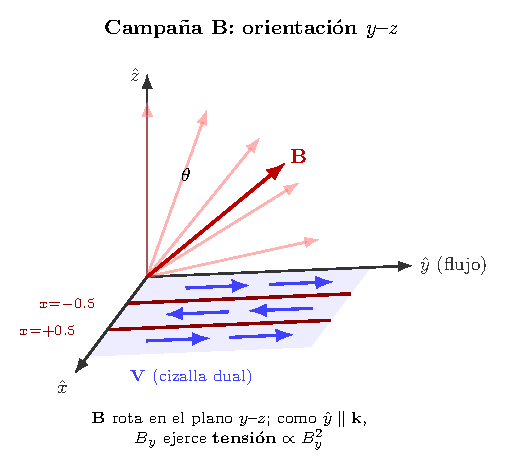
\includegraphics[width=0.32\textwidth]{figures/campana_B_3d.pdf}\hfill
  
\includegraphics[width=0.32\textwidth]{figures/campana_C_3d.pdf}
\end{center}
\end{frame}

%==============================================================================
\section{Marco te\'orico: el sistema RRMHD}
%==============================================================================

%------------------------------------------------------------------------------
% S6 · ESTRUCTURA COVARIANTE
%------------------------------------------------------------------------------
\begin{frame}{Estructura Covariante del Sistema RRMHD}
\framesubtitle{Leyes de conservaci\'on invariantes de Lorentz}
\begin{columns}[T]
\begin{column}{0.48\textwidth}
  \begin{tcolorbox}[RES={Convenciones (v\'alidas en TODA la presentaci\'on)}]
    \scriptsize
    Heaviside--Lorentz: $c=\mu_0=\epsilon_0=1$.\quad
    Signatura: $\eta_{\mu\nu}=\mathrm{diag}(-,+,+,+)$.\\
    $W=(1-v^2)^{-1/2}$ factor de Lorentz;\quad
    $\Gamma$ \emph{solo} \'indice adiab\'atico
    (formulaci\'on de Valencia, \citealp{rezzolla-2013}).
  \end{tcolorbox}
  \vspace{0.1cm}
  \begin{tcolorbox}[EQ={Sistema covariante}]
    \scriptsize
    \begin{align*}
      \partial_\mu(\rho u^\mu) &= 0 && \text{(bariones)}\\
      \partial_\mu T^{\mu\nu} &= 0 && \text{(energ\'ia-momento \emph{total})}\\
      \partial_\mu F^{\mu\nu} &= J^\nu && \text{(Maxwell inhomog\'eneas)}\\
      \partial_\mu(\star F)^{\mu\nu} &= 0 && \text{(identidad de Bianchi)}
    \end{align*}
  \end{tcolorbox}
\end{column}
\begin{column}{0.48\textwidth}
  \begin{tcolorbox}[EQ={Tensor de energ\'ia-momento total}]
    \scriptsize
    \begin{align*}
      T^{\mu\nu} &= T^{\mu\nu}_{\rm fluid}+T^{\mu\nu}_{\rm em}\\[2pt]
      T^{\mu\nu}_{\rm fluid} &= \rho h\,u^\mu u^\nu + p\,\eta^{\mu\nu}\\[2pt]
      T^{\mu\nu}_{\rm em} &= F^{\mu\lambda}F^{\nu}_{\ \lambda}
        -\tfrac14\eta^{\mu\nu}F_{\alpha\beta}F^{\alpha\beta}
    \end{align*}
    Ambos derivados por variaci\'on de la m\'etrica (Hilbert)
    de $S_{\rm em}$ y de la acci\'on de Taub $S_{\rm fluid}=\int p\sqrt{-g}\,d^4x$
    \hfill{\tiny[resp.\ B2]}
  \end{tcolorbox}
  \vspace{0.1cm}
  \begin{block}{Punto geom\'etrico clave}
    \scriptsize
    $F\equiv dA$ (2-forma de Faraday) $\Rightarrow$ $dF=d^2A=0$
    por \textbf{nilpotencia}: la ausencia de monopolos
    ($\nabla\!\cdot\!\mathbf B=0$) es una \textbf{identidad geom\'etrica},
    no una ecuaci\'on din\'amica. Las inhomog\'eneas s\'i son din\'amica
    (m\'inima acci\'on con fuente $J_\mu A^\mu$). \hfill{\tiny[resp.\ B1]}
  \end{block}
\end{column}
\end{columns}
\end{frame}

%------------------------------------------------------------------------------
% S7 · LEY DE OHM RELATIVISTA
%------------------------------------------------------------------------------
\begin{frame}{La Ley de Ohm Relativista: el Cierre Resistivo}
\framesubtitle{La ecuaci\'on constitutiva que define el r\'egimen}
\begin{columns}[T]
\begin{column}{0.50\textwidth}
  \begin{tcolorbox}[EQ={Del marco com\'ovil al laboratorio}]
    \scriptsize
    Covariante (com\'ovil, respuesta lineal e is\'otropa):
    \[
      J^\mu=\rho_e u^\mu+\sigma F^{\mu\nu}u_\nu
    \]
    Proyecci\'on 3+1 sobre la malla euleriana:
    \[
      \boxed{\ \mathbf{J}=\rho_q\mathbf{v}
        +\sigma W\bigl[\mathbf{E}+\mathbf{v}\times\mathbf{B}
        -(\mathbf{E}\cdot\mathbf{v})\mathbf{v}\bigr]\ }
    \]
    {\tiny No es una suma galileana: $W$ y los acoples transversales son
    la huella relativista. \hfill[resp.\ B5]}
  \end{tcolorbox}
  \vspace{0.1cm}
  \begin{tcolorbox}[RES={Los dos l\'imites f\'isicos}]
    \scriptsize
    \begin{itemize}\setlength\itemsep{2pt}
      \item $\sigma\to\infty$: $\mathbf E+\mathbf v\times\mathbf B=0$
            (congelamiento, RMHD ideal).
      \item $0<\sigma<\infty$: sobrevive $\mathbf E'$ com\'ovil
            $\Rightarrow$ Joule ($j^\mu E_\mu>0$) $+$ reconexi\'on.
    \end{itemize}
  \end{tcolorbox}
\end{column}
\begin{column}{0.46\textwidth}
  \begin{tcolorbox}[WRN={Honestidad del cierre: l\'imites de validez}]
    \scriptsize
    \begin{itemize}\setlength\itemsep{2pt}
      \item $\sigma$ \textbf{escalar e is\'otropa}: exige plasma colisional
            ($\nu_{\rm col}\gg\omega_{\rm cicl}$); sin efecto Hall ni
            anisotrop\'ia respecto a $\mathbf B$.
      \item $\eta$ es un \textbf{coeficiente de transporte macrosc\'opico}:
            emerge de las integrales de colisi\'on del nivel cin\'etico
            (Vlasov--Boltzmann). \hfill{\tiny[resp.\ B11]}
      \item La escala micro relevante del modelo es la capa resistiva
            $\delta\sim S^{-1/2}$, no el girorradio.
    \end{itemize}
  \end{tcolorbox}
  \vspace{0.1cm}
  \begin{block}{Consecuencia din\'amica}
    \scriptsize
    El t\'ermino fuente $-\sigma\mathbf E$ vuelve el sistema
    \textbf{r\'igido} (\textit{stiff}) cuando $\sigma\gg1$:
    $\tau_{\rm relax}\sim\sigma^{-1}\ll\Delta t_{\rm CFL}$.
    Este es el reto num\'erico central (Secci\'on 3).
  \end{block}
\end{column}
\end{columns}
\end{frame}

%------------------------------------------------------------------------------
% S8 · GLM
%------------------------------------------------------------------------------
\begin{frame}{Restricciones de Divergencia: el Sistema Aumentado GLM}
\framesubtitle{?`C\'omo se garantiza $\nabla\cdot\mathbf B=0$ sin destruir la causalidad?}
\begin{columns}[T]
\begin{column}{0.46\textwidth}
  \begin{block}{El problema: la malla rompe la geometr\'ia}
    \scriptsize
    En el continuo, $dF=0$ garantiza $\nabla\!\cdot\!\mathbf B=0$
    ($d^2=0$). Los operadores \textbf{discretos no son nilpotentes}
    ($d^2\neq0$): el truncamiento genera monopolos espurios que,
    sin tratamiento, se \emph{acumulan} y destruyen la estabilidad
    \citep{Dedner-2002}.
  \end{block}
  \begin{tcolorbox}[EQ={Soluci\'on GLM: la ecuaci\'on del tel\'egrafo}]
    \scriptsize
    Dos escalares $\Phi,\Psi$ (multiplicadores de Lagrange generalizados)
    acoplan las restricciones a la evoluci\'on. El error $\xi$ obedece
    \[
      \partial_t^2\xi+\kappa\,\partial_t\xi-\nabla^2\xi=0 .
    \]
    \begin{itemize}\setlength\itemsep{1pt}
      \item \textbf{Hiperb\'olico}: propaga a $c_h=1$
            $\Rightarrow$ jam\'as viola el cono de luz.
      \item \textbf{Disipativo}: decae $\propto e^{-\kappa t/2}$.
    \end{itemize}
    {\tiny Origen variacional (acci\'on extendida tipo Stueckelberg)
     y equivalencia con la forma de 1.er orden de Dedner: [resp.\ B3].}
  \end{tcolorbox}
\end{column}
\begin{column}{0.50\textwidth}
  \begin{center}
    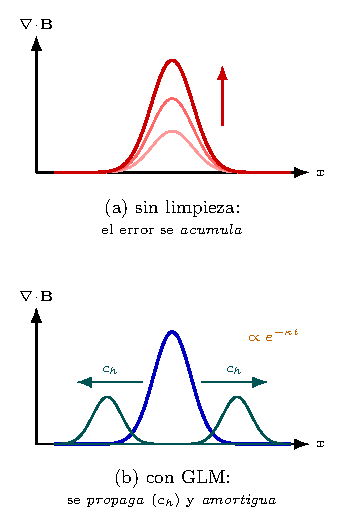
\includegraphics[width=\linewidth]{figures/glm_limpieza.pdf}\\[2pt]
    {\tiny\color{INF3} (a) Sin tratamiento el error se acumula;
     (b) con GLM se \emph{propaga} fuera del dominio a $c_h$ y se
     \emph{amortigua} exponencialmente, sin alterar las soluciones f\'isicas.}
  \end{center}
\end{column}
\end{columns}
\end{frame}

%------------------------------------------------------------------------------
% S9 · SISTEMA CONSERVATIVO 14 VARIABLES
%------------------------------------------------------------------------------
\begin{frame}{El Sistema en Forma Fuertemente Conservativa}
\framesubtitle{$\partial_t\mathbf U+\partial_i\mathbf F^i(\mathbf U)=\mathbf S(\mathbf U)$ --- 14 variables}
\begin{columns}[T]
\begin{column}{0.50\textwidth}
  \begin{tcolorbox}[EQ={Vector de estado (variables \emph{totales})}]
    \scriptsize
    \[
      \mathbf{U}=\bigl(D,\;S^j,\;\tau,\;B^j,\;E^j,\;\rho_q,\;\Psi,\;\Phi\bigr)^{T}
      \quad(14)
    \]
    \vspace{-0.35cm}
    \begin{align*}
      D &= \rho W\\
      S^j &= \rho h W^2 v^j+(\mathbf{E}\times\mathbf{B})^j\\
      \tau &= \tfrac12\!\left(E^2+B^2\right)+\rho h W^2-p
    \end{align*}
  \end{tcolorbox}
  \vspace{0.08cm}
  \begin{block}{Consecuencia de conservar el tensor \emph{total}}
    \scriptsize
    Momento y energ\'ia incluyen el vector de Poynting y
    $\tfrac12(E^2+B^2)$: la \textbf{fuerza de Lorentz no es un t\'ermino
    fuente}, queda absorbida en la divergencia del flujo
    $\Rightarrow$ conservaci\'on exacta a nivel discreto (captura de choques).
  \end{block}
\end{column}
\begin{column}{0.46\textwidth}
  \begin{tcolorbox}[EQ={Vector fuente}]
    \scriptsize
    \[
      \mathbf{S}(\mathbf U)=\bigl(0,\;-\Psi B^j,\;-\Psi(\mathbf v\!\cdot\!\mathbf B),\;
      0,\;-J^j,\;0,\;-\kappa_B\Psi,\;\rho_q-\kappa_E\Phi\bigr)^{T}
    \]
    \begin{itemize}\setlength\itemsep{1pt}
      \item $-J^j$: cierre de Ohm (\'unico acople resistivo).
      \item $-\Psi B^j$, $-\Psi(\mathbf v\!\cdot\!\mathbf B)$: t\'erminos de
            \textbf{Godunov--Powell} --- compensan la aceleraci\'on
            artificial de los monopolos transitorios y preservan la
            compatibilidad termodin\'amica \citep{ruedaramirez2023}.
    \end{itemize}
  \end{tcolorbox}
  \vspace{0.08cm}
  \begin{tcolorbox}[HYP={Estructura caracter\'istica}]
    \scriptsize
    Jacobiano $\mathbf A_{14\times14}=\partial\mathbf F/\partial\mathbf U$:
    \textbf{14 autovalores}, 8 degenerados a $\pm c$ (sector EM $+$ GLM);
    el resto: magnetos\'onicas r\'apidas, entrop\'ia/cizalla y carga
    \citep{miranda-aranguren-2018}. \hfill{\tiny[resp.\ B4]}
  \end{tcolorbox}
\end{column}
\end{columns}
\end{frame}

%------------------------------------------------------------------------------
% S10 · MAPA DE LÍMITES
%------------------------------------------------------------------------------
\begin{frame}{Mapa de L\'imites: del RRMHD a la F\'isica Conocida}
\framesubtitle{Cada l\'imite recupera una teor\'ia consolidada --- y una versi\'on de la KHI}
\begin{center}
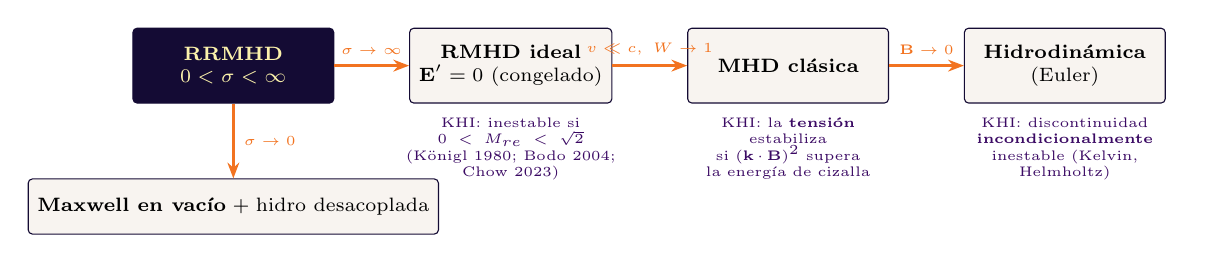
\begin{tikzpicture}[
  box/.style={draw=primary,fill=bgwarm,rounded corners=1.5pt,align=center,
              minimum width=2.55cm,minimum height=0.95cm,font=\scriptsize},
  hbox/.style={box,fill=primary,text=soft},
  lim/.style={-{Stealth[length=2mm]},very thick,accent},
  note/.style={align=center,font=\tiny,text width=2.75cm,color=INF2}]
  \node[hbox] (rrmhd) {\textbf{RRMHD}\\$0<\sigma<\infty$};
  \node[box,right=0.95cm of rrmhd] (rmhd) {\textbf{RMHD ideal}\\$\mathbf E'=0$ (congelado)};
  \node[box,right=0.95cm of rmhd] (mhd) {\textbf{MHD cl\'asica}};
  \node[box,right=0.95cm of mhd] (hidro) {\textbf{Hidrodin\'amica}\\(Euler)};
  \draw[lim] (rrmhd) -- node[above,font=\tiny\bfseries]{$\sigma\to\infty$} (rmhd);
  \draw[lim] (rmhd) -- node[above,font=\tiny\bfseries]{$v\ll c,\ W\to1$} (mhd);
  \draw[lim] (mhd) -- node[above,font=\tiny\bfseries]{$\mathbf B\to0$} (hidro);
  \node[box,below=0.95cm of rrmhd,minimum height=0.7cm] (vacio)
    {\textbf{Maxwell en vac\'io}$\;+\;$hidro desacoplada};
  \draw[lim] (rrmhd) -- node[right,font=\tiny\bfseries]{$\sigma\to0$} (vacio);
  \node[note,below=1.5pt of rmhd]{KHI: inestable si\\ $0<M_{re}<\sqrt2$\\
    {\tiny(K\"onigl 1980; Bodo 2004;\\ Chow 2023)}};
  \node[note,below=1.5pt of mhd]{KHI: la \textbf{tensi\'on} estabiliza\\
    si $(\mathbf k\!\cdot\!\mathbf B)^2$ supera\\ la energ\'ia de cizalla};
  \node[note,below=1.5pt of hidro]{KHI: discontinuidad\\
    \textbf{incondicionalmente}\\ inestable {\tiny(Kelvin, Helmholtz)}};
\end{tikzpicture}
\end{center}
\vspace{0.05cm}
\begin{tcolorbox}[WRN={El punto que define esta tesis}]
  \scriptsize
  En RRMHD \textbf{no existe relaci\'on de dispersi\'on algebraica cerrada}
  para la discontinuidad tangencial: el t\'ermino $\eta\nabla^2\mathbf B$ es
  \emph{parab\'olico} y suaviza la interfaz en tiempo arbitrariamente corto,
  invalidando el empalme cl\'asico de soluciones \citep{palenzuela-2009}.
  $\Rightarrow$ la tasa de crecimiento $\gamma_{\rm KHI}(\sigma)$ debe
  caracterizarse \textbf{num\'ericamente}; la teor\'ia lineal RMHD
  compresible se usa como referencia del l\'imite ideal.
\end{tcolorbox}
\end{frame}

%------------------------------------------------------------------------------
% S11 · OBSERVABLE: ENSTROFÍA
%------------------------------------------------------------------------------
\begin{frame}{El Observable: Vorticidad y Enstrof\'ia de Perturbaci\'on}
\framesubtitle{C\'omo se mide $\gamma_{\rm KHI}$ sin contaminaci\'on del flujo base}
\begin{columns}[T]
\begin{column}{0.50\textwidth}
  \begin{tcolorbox}[EQ={Construcci\'on del estimador}]
    \scriptsize
    Vorticidad perturbada (se sustrae la cizalla base):
    \[
      \omega_z'(x,y,t)=\omega_z-\bigl\langle\omega_z(t{=}0)\bigr\rangle_y,
      \qquad \omega_z=\partial_xV_y-\partial_yV_x
    \]
    Enstrof\'ia de perturbaci\'on:
    \[
      \Omega_{zp}(t)=\int(\omega_z')^2\,dA
    \]
    En fase lineal cada modo crece $\propto e^{\gamma_{\rm KHI}t}$
    y la enstrof\'ia es \textbf{cuadr\'atica} en la amplitud:
    \[
      \boxed{\ \ln\Omega_{zp}(t)=a+2\,\gamma_{\rm KHI}\,t\ }
    \]
    $\Rightarrow$ regresi\'on lineal en la ventana can\'onica
    $t\in[2.4,\,3.4]$; la pendiente es $2\gamma_{\rm KHI}$
    \citep{nastro2022}.
  \end{tcolorbox}
\end{column}
\begin{column}{0.46\textwidth}
  \begin{block}{Diagn\'osticos complementarios}
    \scriptsize
    \begin{itemize}\setlength\itemsep{2pt}
      \item $\Omega_{\rm tot}(t)$ y fracci\'on fuera del plano
            $f_{Vz}=(\Omega_{\rm tot}-\Omega_z)/\Omega_{\rm tot}$:
            estructuras secundarias 3D.
      \item $J_{\max}(t)$: adelgazamiento de l\'aminas de corriente.
      \item $\int\mathbf E\cdot\mathbf J\,dA$: disipaci\'on \'ohmica global.
      \item $E_{\rm mag}$, $E_{\rm kin}$, $E_{\rm int}$: balance
            e intercambio energ\'etico.
    \end{itemize}
  \end{block}
  \vspace{0.1cm}
  \begin{tcolorbox}[RES={Normalizaci\'on para comparar con la literatura}]
    \scriptsize
    Tasa adimensional:
    $\hat\omega=\gamma_{\rm KHI}\,a_{kh}/v_{\rm sh}$
    (tiempo de tr\'ansito de cizalla).\\
    Se reserva $\sigma$ \emph{exclusivamente} para la conductividad.
  \end{tcolorbox}
\end{column}
\end{columns}
\end{frame}

%==============================================================================
\section{Implementaci\'on num\'erica y montaje experimental}
%==============================================================================

%------------------------------------------------------------------------------
% S12 · VOLÚMENES FINITOS
%------------------------------------------------------------------------------
\begin{frame}{Volumenes Finitos: la Formulaci\'on Integral Obligatoria}
\framesubtitle{Por qu\'e FVM para leyes de conservaci\'on relativistas}
\begin{columns}[T]
\begin{column}{0.48\textwidth}
  \begin{tcolorbox}[EQ={Promedios de celda y flujos de interfaz}]
    \scriptsize
    \[
      \frac{d\bar{\mathbf U}_i}{dt}
      =-\frac{1}{\Delta x}\Bigl[\hat{\mathbf F}_{i+1/2}-\hat{\mathbf F}_{i-1/2}\Bigr]
      +\bar{\mathbf S}_i
    \]
    La conservaci\'on es \textbf{exacta por construcci\'on}: el flujo que
    sale de una celda entra \'integramente en la vecina.
  \end{tcolorbox}
  \vspace{0.1cm}
  \begin{block}{Por qu\'e la forma integral y no la diferencial}
    \scriptsize
    En flujos relativistas emergen \textbf{choques} que vuelven singular la
    forma diferencial. La forma integral admite soluciones d\'ebiles y los
    flujos num\'ericos respetan las condiciones de salto de
    \textbf{Rankine--Hugoniot} \citep{toro-2009}.\\[3pt]
    {\color{INF3}(FEM --- formulaci\'on d\'ebil global --- es \'optimo para
    dominios complejos con soluciones suaves; para sistemas hiperb\'olicos
    con discontinuidades, la captura conservativa de choques exige FVM.)}
  \end{block}
\end{column}
\begin{column}{0.48\textwidth}
  \begin{center}
    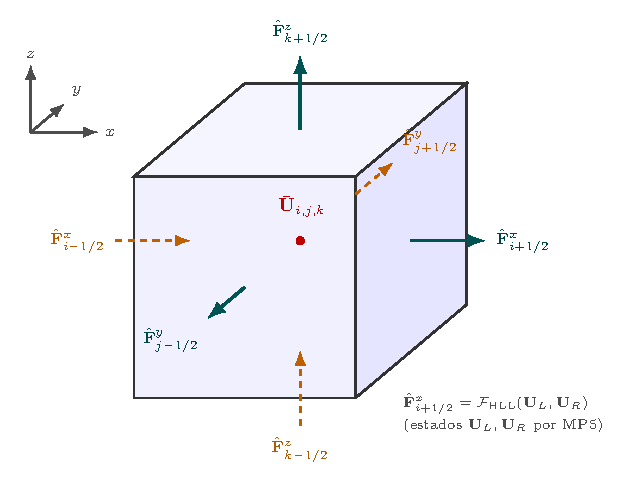
\includegraphics[width=0.9\linewidth]{figures/celda_3d_flujos.pdf}\\[2pt]
    {\tiny\color{INF3} Celda $(i,j,k)$: la evoluci\'on del promedio
     $\bar{\mathbf U}$ es el balance de los flujos de Riemann en sus seis
     caras.}
  \end{center}
\end{column}
\end{columns}
\end{frame}

%------------------------------------------------------------------------------
% S13 · MP5 + HLL
%------------------------------------------------------------------------------
\begin{frame}{Reconstrucci\'on MP5 $+$ Solucionador HLL}
\framesubtitle{El control expl\'icito de la difusi\'on num\'erica}
\begin{columns}[T]
\begin{column}{0.52\textwidth}
  \begin{block}{Reconstrucci\'on de 5.º orden \citep{suresh-1997}}
    \scriptsize
    Teorema de Godunov: alto orden lineal $\Rightarrow$ oscilaciones
    (Gibbs). Los TVD de 2.º orden las evitan pero \emph{recortan} los
    extremos $\Rightarrow$ matan la enstrof\'ia. \textbf{MP5}: stencil de 5
    puntos $+$ mediana proyectiva
    $\mathbf U_L=\mathrm{median}(\mathbf U^{(5)},\mathbf U_{\min},\mathbf U_{\max})$
    $\Rightarrow$ retenci\'on casi espectral de la vorticidad.
  \end{block}
  \begin{tcolorbox}[EQ={Flujo HLL (libre de jacobianos)}]
    \scriptsize
    \[
      \mathbf F^{hll}=\frac{\lambda_R\mathbf F_L-\lambda_L\mathbf F_R
        +\lambda_L\lambda_R(\mathbf U_R-\mathbf U_L)}{\lambda_R-\lambda_L}
    \]
    Robusto y positivo; su difusi\'on sobre la onda de contacto la
    \textbf{compensa la agudeza de los estados MP5}
    \citep{miranda-aranguren-2018}. \hfill{\tiny[resp.\ B7: ?`y HLLC?]}
  \end{tcolorbox}
\end{column}
\begin{column}{0.44\textwidth}
  \begin{center}
    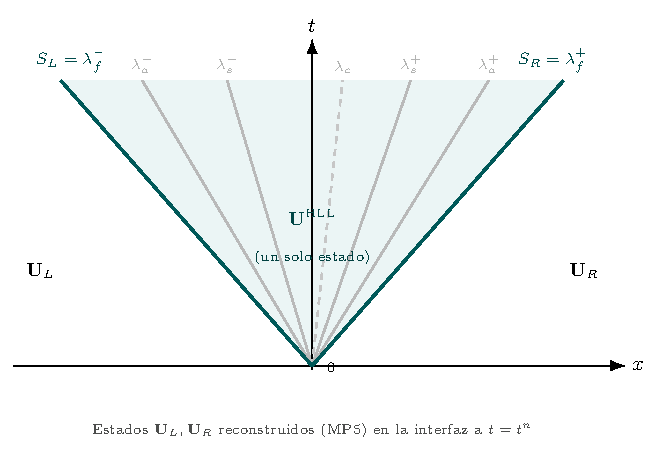
\includegraphics[width=\linewidth]{figures/riemann_hll.pdf}
  \end{center}
  \vspace{-0.1cm}
  \begin{tcolorbox}[RES={Criterio de dise\~no del estudio}]
    \scriptsize
    \textbf{Disipaci\'on num\'erica $<$ disipaci\'on f\'isica $\eta$}
    en todo el barrido: la KHI debe crecer y reconectar por la f\'isica,
    no por la malla. (Evidencia emp\'irica: plateau de $J_{\max}$,
    Secci\'on de resultados.)
  \end{tcolorbox}
\end{column}
\end{columns}
\end{frame}

%------------------------------------------------------------------------------
% S14 · IMEX
%------------------------------------------------------------------------------
\begin{frame}{Rigidez Resistiva e Integraci\'on IMEX--RK}
\framesubtitle{C\'omo se integra un sistema con $\tau_{\rm relax}\sim\sigma^{-1}\ll\Delta t_{\rm CFL}$}
\begin{columns}[T]
\begin{column}{0.50\textwidth}
  \begin{block}{Partici\'on de operadores \citep{pareschi-2005}}
    \scriptsize
    \begin{itemize}\setlength\itemsep{2pt}
      \item \textbf{Expl\'icito}: flujos hiperb\'olicos $-\partial_i\mathbf F^i$
            (MP5 $+$ HLL), $\Delta t\propto\Delta x$.
      \item \textbf{Impl\'icito}: fuente r\'igida $-\sigma\mathbf E$.
            Sin acople intercelular $\Rightarrow$ sistema
            \textbf{algebraico local $3\times3$ con soluci\'on anal\'itica}
            (no hay Newton global ni inversi\'on matricial iterativa).
    \end{itemize}
  \end{block}
  \begin{tcolorbox}[RES={Preservaci\'on asint\'otica (l\'imite ideal exacto)}]
    \scriptsize
    De la actualizaci\'on impl\'icita
    $\mathbf E^{(i)}+\alpha\sigma W[\mathbf E^{(i)}-(\mathbf v\!\cdot\!\mathbf E^{(i)})\mathbf v]
     =\mathbf E^*-\alpha\sigma W(\mathbf v\times\mathbf B)$,
    dividiendo por $\alpha\sigma W$ y tomando $\sigma\to\infty$:
    \[
      \mathbf E\to-\mathbf v\times\mathbf B
    \]
    El esquema \textbf{converge por construcci\'on a la ley de Ohm ideal}:
    sin p\'erdida de estabilidad ni $\Delta t$ prohibitivos.
  \end{tcolorbox}
\end{column}
\begin{column}{0.46\textwidth}
  \begin{center}
    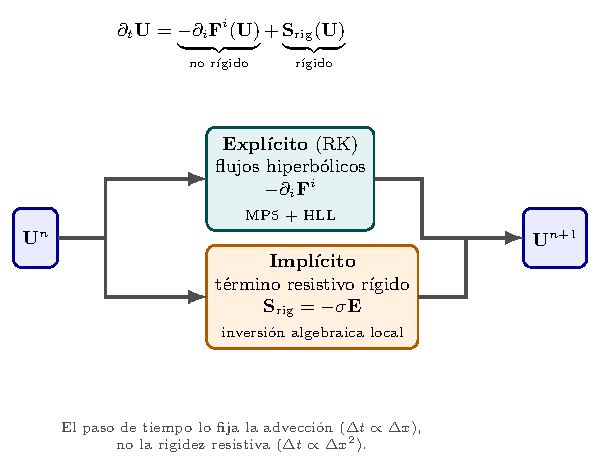
\includegraphics[width=\linewidth]{figures/imex_splitting.pdf}\\[2pt]
    {\tiny\color{INF3} Partici\'on IMEX: advecci\'on expl\'icita
     ($\Delta t\propto\Delta x$) $+$ fuente resistiva impl\'icita
     (evita $\Delta t\propto\Delta x^2/\sigma$).}
  \end{center}
\end{column}
\end{columns}
\end{frame}

%------------------------------------------------------------------------------
% S15 · RECUPERACIÓN DE PRIMITIVAS
%------------------------------------------------------------------------------
\begin{frame}{Recuperaci\'on de Variables Primitivas: Ferrari--Cardano}
\framesubtitle{La inversi\'on $\mathbf U\to\mathbf P$ no tiene forma cerrada general\ldots pero s\'i anal\'itica}
\begin{columns}[T]
\begin{column}{0.50\textwidth}
  \begin{block}{El problema}
    \scriptsize
    Los flujos requieren las primitivas
    $\mathbf P=(\rho,v^j,p,B^j,E^j,\rho_q,\Psi,\Phi)$, pero $W=(1-v^2)^{-1/2}$
    acopla cinem\'atica y termodin\'amica: el mapeo $\mathbf U(\mathbf P)$
    carece de inversa expl\'icita directa.
  \end{block}
  \begin{tcolorbox}[EQ={Reducci\'on a una cu\'artica en $W$}]
    \scriptsize
    Con $C_2=\tau-\tfrac12(E^2+B^2)$,\;
    $C_1=|\mathbf S-\mathbf E\times\mathbf B|^2$,\; $D$ y la EoS politr\'opica:
    \[
      W^4+b_3W^3+b_2W^2+b_1W+b_0=0
    \]
    \begin{enumerate}\setlength\itemsep{1pt}
      \item Transformaci\'on de \textbf{Tschirnhaus} $\to$ cu\'artica reducida;
      \item soluci\'on \textbf{anal\'itica} de Ferrari--Cardano
            $\to$ ra\'iz f\'isicamente admisible;
      \item refinamiento con pocas iteraciones de Newton--Raphson.
    \end{enumerate}
  \end{tcolorbox}
\end{column}
\begin{column}{0.46\textwidth}
  \begin{tcolorbox}[WRN={Guardias f\'isicas del algoritmo}]
    \scriptsize
    \begin{itemize}\setlength\itemsep{2pt}
      \item Rechazo de velocidades superlum\'inicas ($v^2\ge1$).
      \item Rechazo de presiones no positivas ($p\le0$).
      \item Rama linealizada estable para $v^2\lesssim10^{-2}$.
      \item \textit{Fallback} a promedios de celdas vecinas si la ra\'iz
            es inadmisible.
    \end{itemize}
  \end{tcolorbox}
  \vspace{0.12cm}
  \begin{block}{Por qu\'e importa}
    \scriptsize
    La recuperaci\'on se ejecuta \textbf{en cada celda y en cada subpaso}
    del integrador: su robustez frente a estados extremos (l\'aminas de
    corriente agudas a alta $\sigma$) es la que define el l\'imite pr\'actico
    del barrido en conductividad --- y explica los fallos de las
    configuraciones magn\'eticas d\'ebiles excluidas de la Campa\~na A.
  \end{block}
\end{column}
\end{columns}
\end{frame}

%------------------------------------------------------------------------------
% S16 · SETUP
%------------------------------------------------------------------------------
\begin{frame}{Montaje Experimental: Doble Capa de Cizalla tipo Mizuno}
\framesubtitle{Condiciones iniciales \citep{mizuno-2013} --- Test 35A}
\begin{columns}[T]
\begin{column}{0.55\textwidth}
  \begin{center}
    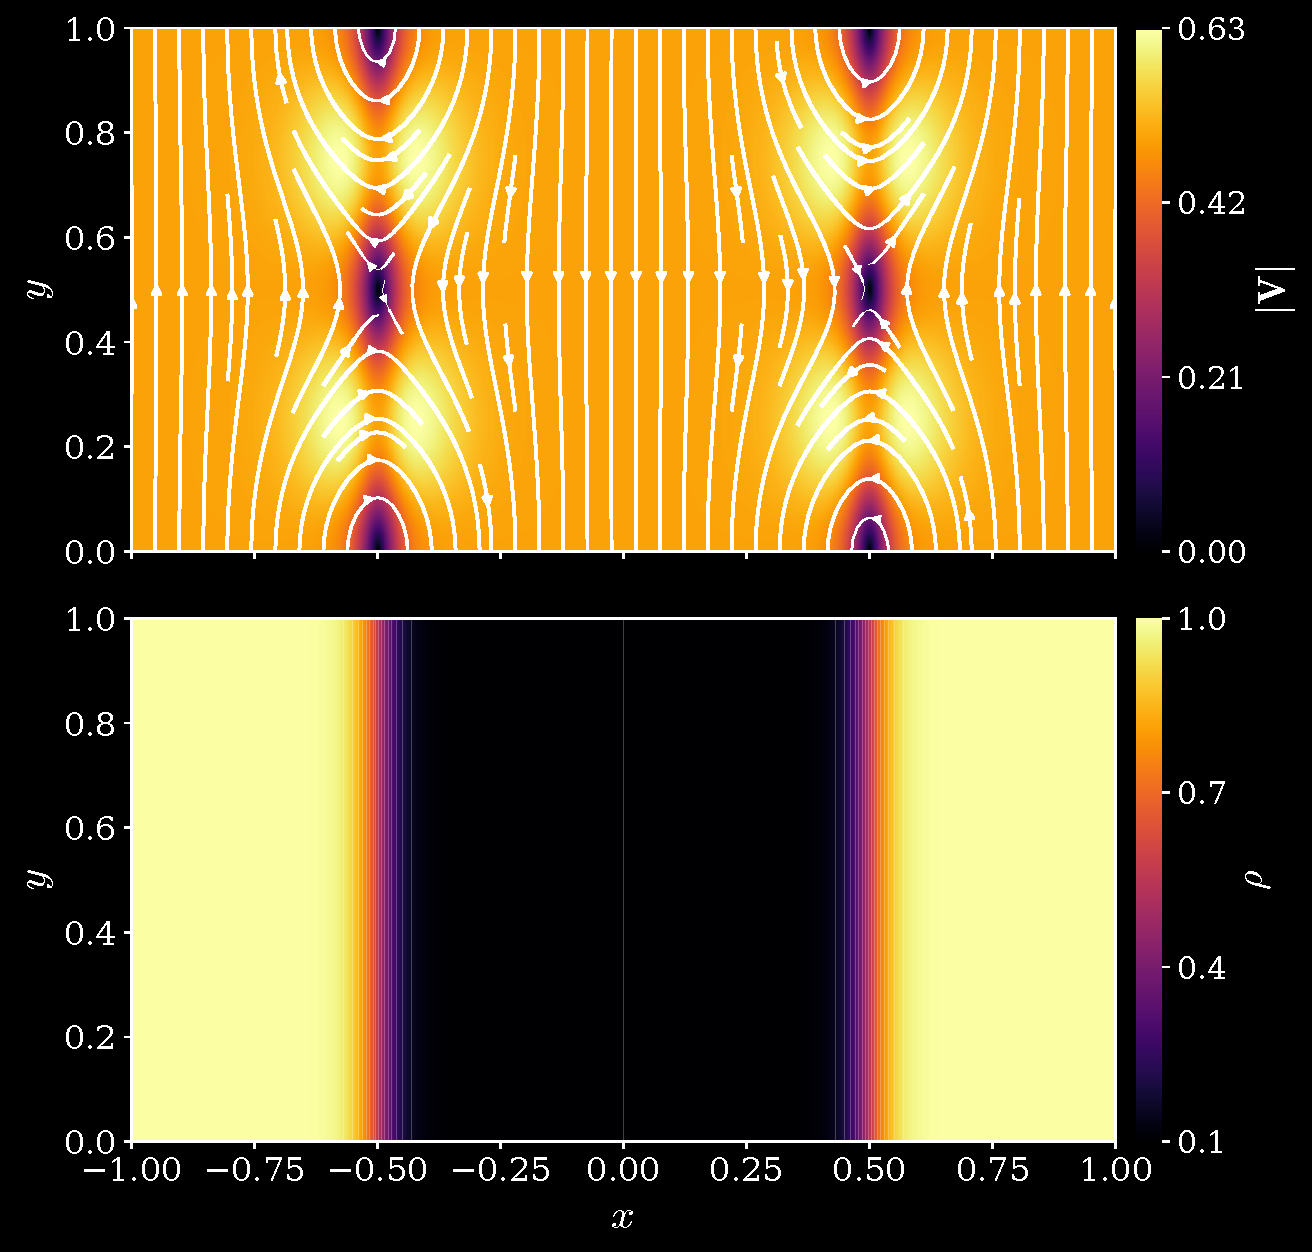
\includegraphics[height=0.63\textheight]{figures/setup_inicial_slide.pdf}\\[2pt]
    {\tiny\color{INF3} $t=0$: (arriba) l\'ineas de corriente sobre $|\mathbf V|$,
     capas en $x=\pm0.5$; (abajo) $\rho$: flujo central diluido
     ($\eta_\rho=0.1$) en ambiente denso --- modela chorro/medio, las
     interfaces son rectas.}
  \end{center}
\end{column}
\begin{column}{0.42\textwidth}
  \begin{tcolorbox}[EQ={Estado base y semilla}]
    \scriptsize
    \begin{itemize}\setlength\itemsep{1pt}
      \item $V_y(x)=\pm v_{\rm sh}\tanh[(x\mp0.5)/a_{kh}]$;\;
            $v_{\rm sh}=0.5$, $a_{kh}=0.05$.
      \item \textbf{Semilla}: perturbaci\'on senoidal en $V_x$
            (modo fundamental $k=2\pi/L_y$, confinamiento gaussiano)
            --- \emph{no} el perfil de densidad.
      \item $\mathbf B=(0,\sqrt{0.02},\sqrt{2.0})$: \textbf{campo gu\'ia}
            $B_z$ dominante (presi\'on, no tensi\'on:
            $\mathbf k\cdot\mathbf B\propto B_y$ d\'ebil)
            $\Rightarrow$ la KHI puede desarrollarse y se a\'isla
            el efecto resistivo.
      \item $\mathbf E(0)=0$: Ohm relaja el sistema al r\'egimen
            consistente con $\sigma$.
    \end{itemize}
  \end{tcolorbox}
  \vspace{0.08cm}
  \begin{tcolorbox}[RES={Dominio y escalas}]
    \scriptsize
    Malla $512\times256$ en $[-1,1]\times[-0.5,0.5]$
    ($\approx13$ celdas/capa); peri\'odica en $y$, abierta en $x$;
    $\Gamma=4/3$; CFL $=0.1$.\\
    Escala astrof\'isica: con $L_0=10^{16}$ cm,
    $\tau_c\approx3.8$ d\'ias; $t=5\approx19$ d\'ias de un jet de AGN;
    v\'ortice maduro $\sim170$ UA.
  \end{tcolorbox}
\end{column}
\end{columns}
\end{frame}

%------------------------------------------------------------------------------
% S17 · MATRIZ DE CAMPAÑAS Y TRANSPARENCIA
%------------------------------------------------------------------------------
\begin{frame}{Matriz de Simulaciones y Criterios de Exclusi\'on}
\framesubtitle{Qu\'e se corri\'o, con qu\'e CFL, y qu\'e se excluy\'o (y por qu\'e)}
\begin{columns}[T]
\begin{column}{0.50\textwidth}
  \begin{tcolorbox}[EQ={Matriz $\sigma\times$CFL}]
    \scriptsize
    \begin{tabular}{@{}lll@{}}
      \toprule
      Campa\~na & $\sigma$ & CFL\\
      \midrule
      Barrido (44) & $100\ldots10\,500$ & $0.10$\\
      Magn\'etica A/B/C & $6000$ & $0.04$\\
      Magn\'etica A/B/C & $10\,000$ & $0.02$\\
      \bottomrule
    \end{tabular}\\[4pt]
    A alta $\sigma$ y campo fuerte las l\'aminas de corriente agudizan la
    recuperaci\'on de primitivas $\Rightarrow$ reducir el CFL estabiliza
    esas corridas.
  \end{tcolorbox}
  \vspace{0.1cm}
  {\scriptsize $\approx3\times10^4$ horas-n\'ucleo acumuladas;
   horizonte $t>5$ (fase lineal $+$ no lineal $+$ saturaci\'on).}
\end{column}
\begin{column}{0.46\textwidth}
  \begin{tcolorbox}[WRN={Datos excluidos --- declarados y justificados}]
    \scriptsize
    \begin{itemize}\setlength\itemsep{2pt}
      \item \textbf{Campa\~na A}: $B_0=0.25,\,0.5$ fallaron por
            inestabilidad num\'erica antes de la fase no lineal
            $\Rightarrow$ el an\'alisis usa $B_0\in\{1.0,1.5,2.0\}$.
      \item \textbf{Campa\~na B}: $\theta=15^\circ$ se detuvo por fallo de
            convergencia del solucionador de primitivas
            $\Rightarrow$ excluida del conjunto limpio.
      \item \textbf{Barrido}: el an\'alisis cuantitativo de $\gamma_{\rm KHI}$
            usa $\sigma\ge1600$ ($R^2\ge0.90$); las corridas resistivas
            extremas se conservan solo para clasificar el r\'egimen.
    \end{itemize}
  \end{tcolorbox}
\end{column}
\end{columns}
\end{frame}

%==============================================================================
\section{Resultados I: barrido en conductividad}
%==============================================================================

%------------------------------------------------------------------------------
% S18 · VISIÓN GLOBAL
%------------------------------------------------------------------------------
\begin{frame}{Visi\'on Global del Barrido: Fenomenolog\'ia}
\framesubtitle{$\rho(x,y)$ en tres reg\'imenes $\times$ tres instantes --- 44 simulaciones estables hasta $t>5$}
\begin{columns}[T]
\begin{column}{0.60\textwidth}
  \begin{center}
    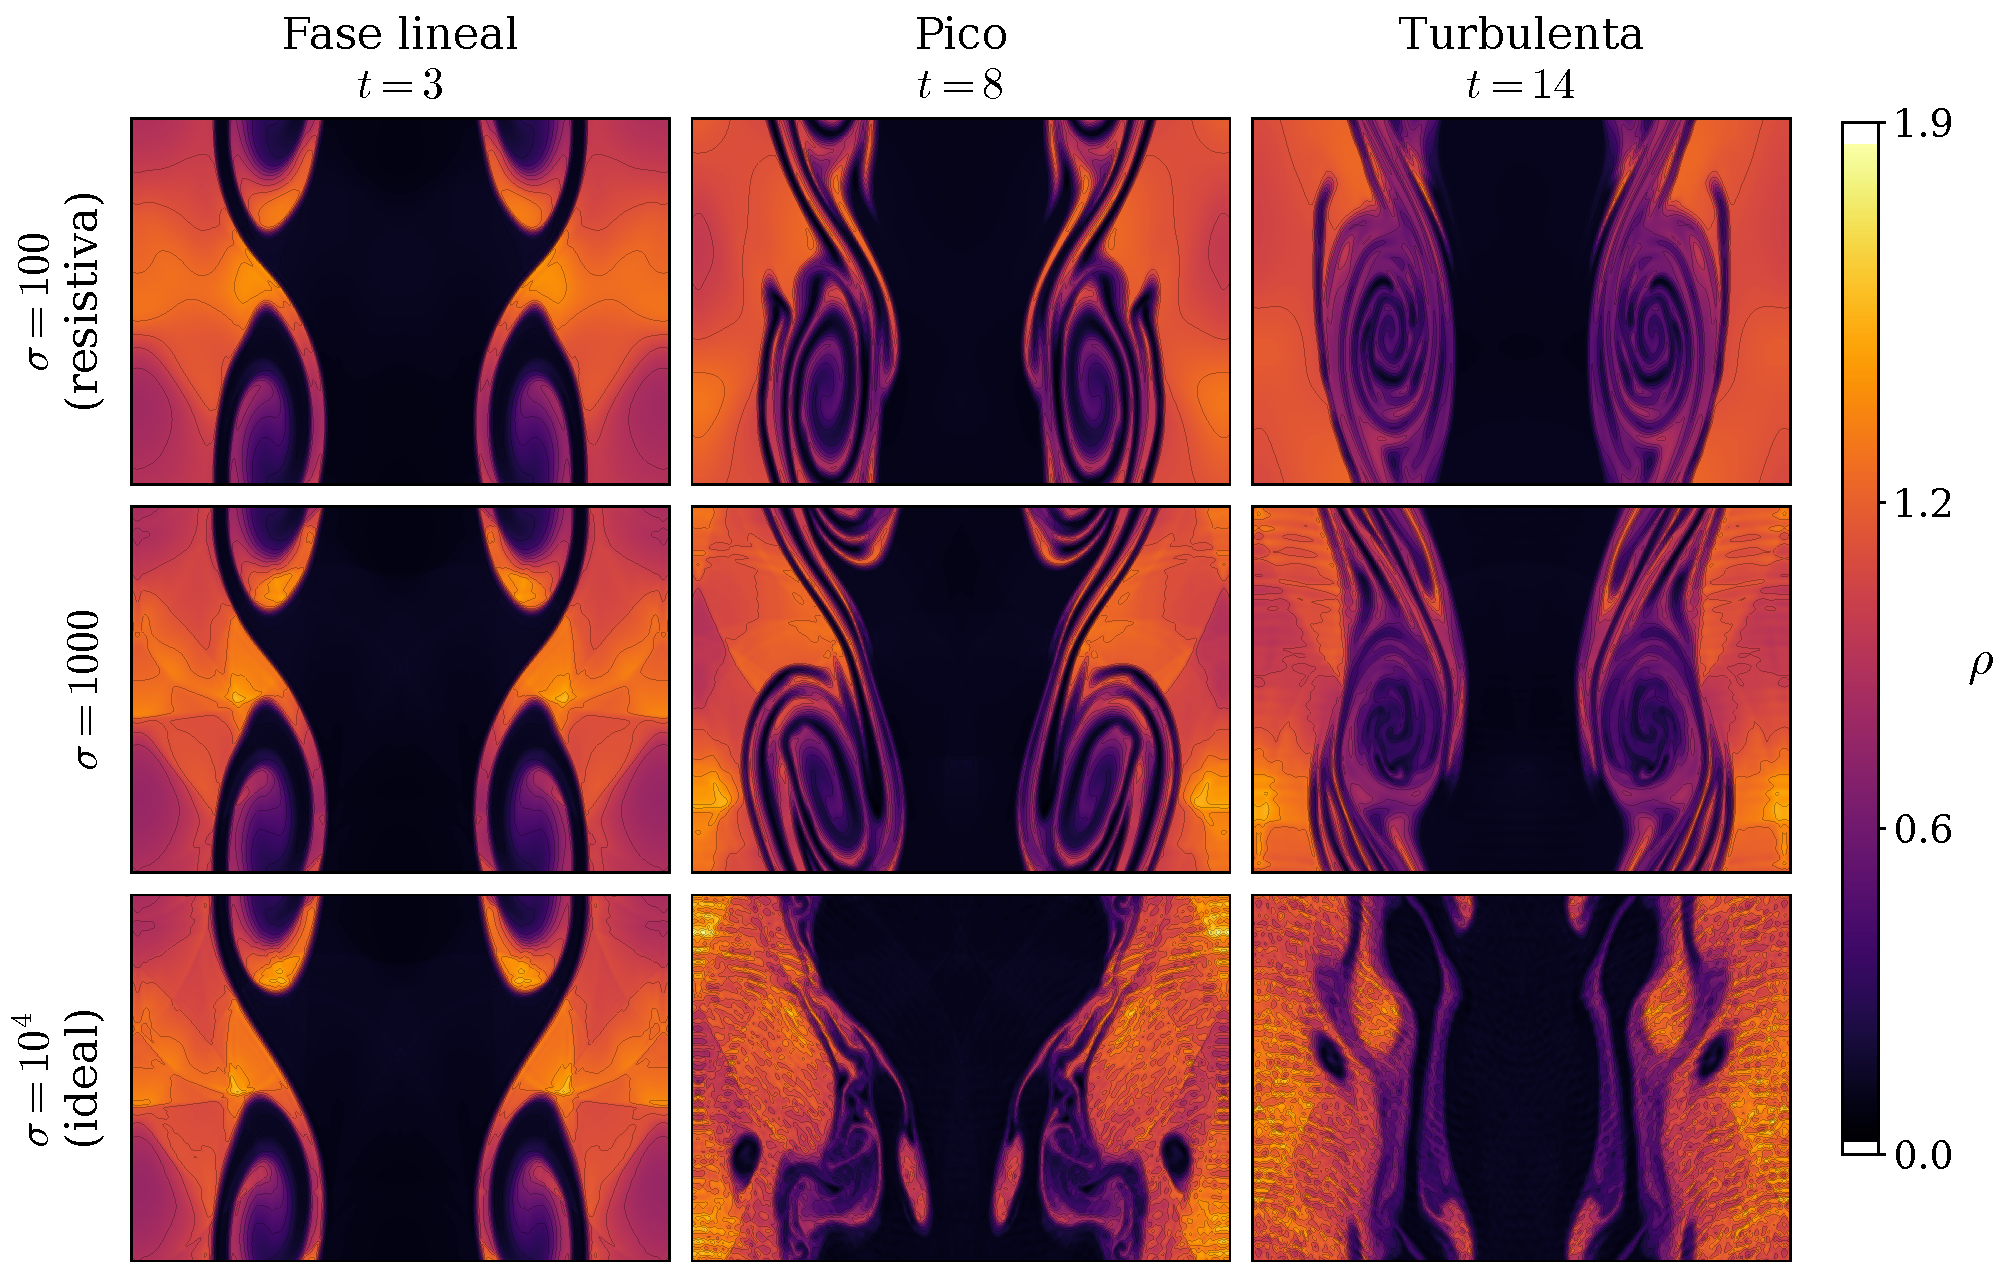
\includegraphics[width=\linewidth]{figures/fig_conductividad_rho_collage_slide.pdf}
  \end{center}
\end{column}
\begin{column}{0.38\textwidth}
  \vspace{0.4cm}
  \begin{block}{Lectura fenomenol\'ogica}
    \scriptsize
    \begin{itemize}\setlength\itemsep{3pt}
      \item Tres fases en todos los casos: \textbf{lineal} ($t\sim3$)
            $\to$ \textbf{enrollamiento no lineal} ($t\sim8$)
            $\to$ \textbf{saturaci\'on} ($t\sim14$).
      \item $\sigma=100$ (resistivo): la difusi\'on \'ohmica amortigua
            y \emph{difumina} los v\'ortices.
      \item $\sigma=10^4$ (cuasi-ideal): campo casi congelado,
            subestructura fina y turbulencia de peque\~na escala.
    \end{itemize}
  \end{block}
  \vspace{0.1cm}
  {\scriptsize\color{INF3} Las 44 simulaciones alcanzaron $t>5$ sin
   inestabilidades num\'ericas espurias; la estratificaci\'on de las curvas
   con $\sigma$ es mon\'otona y limpia.}
\end{column}
\end{columns}
\end{frame}

%------------------------------------------------------------------------------
% S19 · EXTRACCIÓN DE GAMMA
%------------------------------------------------------------------------------
\begin{frame}{Extracci\'on de la Tasa de Crecimiento Lineal}
\framesubtitle{$\ln\Omega_{zp}(t)$: pendiente $=2\gamma_{\rm KHI}$ en la ventana can\'onica}
\begin{columns}[T]
\begin{column}{0.60\textwidth}
  \begin{center}
    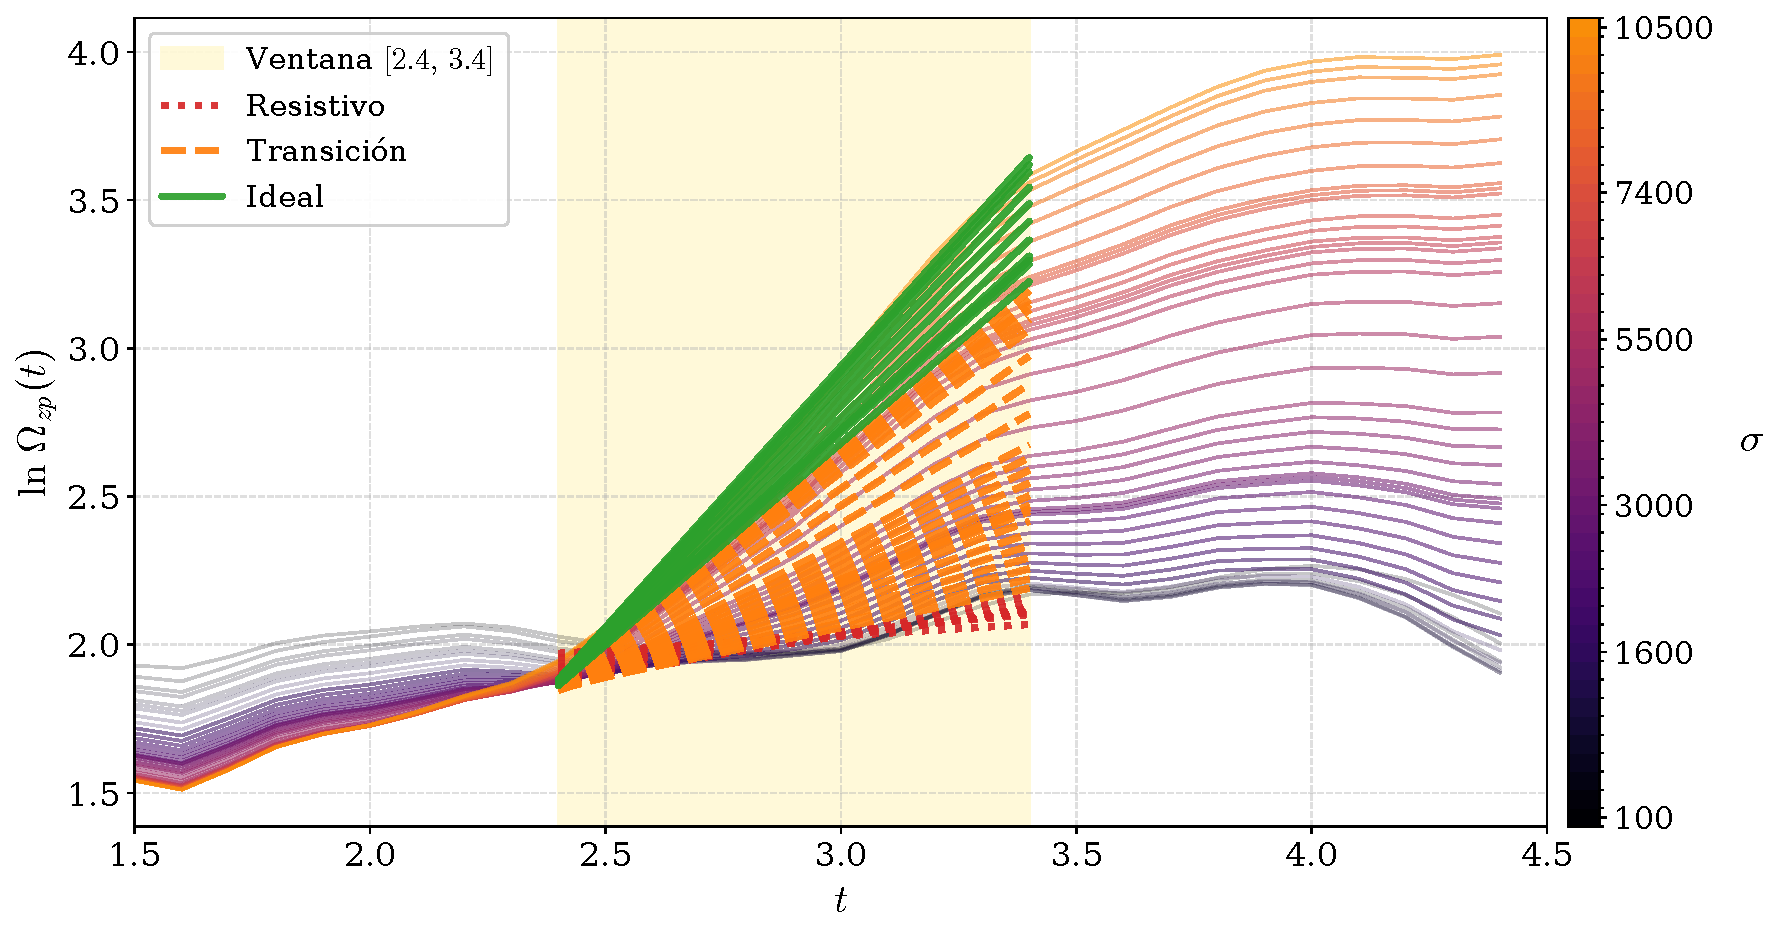
\includegraphics[width=\linewidth]{figures/ln_omega_vs_t_slide.pdf}
  \end{center}
\end{column}
\begin{column}{0.38\textwidth}
  \begin{block}{Criterios de calidad (expl\'icitos)}
    \scriptsize
    \begin{itemize}\setlength\itemsep{2pt}
      \item Ventana fija $t\in[2.4,3.4]$: posterior al transitorio,
            anterior a la saturaci\'on.
      \item Clasificaci\'on por $R^2$: resistivo ($<0.90$),
            transici\'on ($0.90$--$0.995$), ideal ($\ge0.995$).
      \item An\'alisis cuantitativo: $35$ sims con $\sigma\ge1600$.
    \end{itemize}
  \end{block}
  \begin{tcolorbox}[WRN={Precisi\'on conceptual}]
    \scriptsize
    A $\sigma\lesssim1400$ \textbf{no hay fase lineal limpia}: la difusi\'on
    domina desde $t=0$. No es un ``ajuste pobre'': es f\'isica
    --- el modo no alcanza a establecerse.
  \end{tcolorbox}
\end{column}
\end{columns}
\end{frame}

%------------------------------------------------------------------------------
% S20 · SIGMOIDE CON OFFSET
%------------------------------------------------------------------------------
\begin{frame}{La Transici\'on Resistivo$\,\to\,$Ideal: Sigmoide con \emph{Offset}}
\framesubtitle{Objetivo 1 --- resultado param\'etrico central}
\begin{columns}[T]
\begin{column}{0.58\textwidth}
  \begin{center}
    
\includegraphics[width=\linewidth]{figures/fig1_ajuste_v6.pdf}
  \end{center}
\end{column}
\begin{column}{0.40\textwidth}
  \begin{tcolorbox}[EQ={Modelo de 4 par\'ametros}]
    \scriptsize
    \[
      \gamma_{\rm KHI}(\sigma)=C+\frac{\gamma_0}{1+e^{-k(\sigma-\sigma_0)}}
    \]
    \[
      \boxed{\ \gamma_{\rm KHI}(\sigma\!\to\!\infty)=C+\gamma_0=1.03\pm0.05\ }
    \]
    $\sigma_0=2815\pm123$ (centro de la transici\'on).
  \end{tcolorbox}
  \vspace{0.08cm}
  \begin{tcolorbox}[RES={Validaci\'on (sin sobreajuste)}]
    \scriptsize
    \begin{itemize}\setlength\itemsep{2pt}
      \item \textbf{AIC anidado} (mismos datos, $+1$ par\'ametro):
            $\Delta\mathrm{AIC}=-126$ --- evidencia decisiva.
      \item \textbf{Hold-out}: los 9 puntos resistivos NO usados en el
            ajuste se predicen un $36\%$ mejor
            (RMSE $0.039\to0.025$).
      \item Residuos autocorrelacionados $\Rightarrow$ el error formal
            \emph{subestima}: por eso $\sigma_{\rm crit}$ se estima con
            m\'ultiples m\'etodos (siguiente l\'amina). \hfill{\tiny[resp.\ B8]}
    \end{itemize}
  \end{tcolorbox}
\end{column}
\end{columns}
\end{frame}

%------------------------------------------------------------------------------
% S21 · ZONA DE TRANSICIÓN
%------------------------------------------------------------------------------
\begin{frame}{$\sigma_{\rm crit}$ No Es un N\'umero: Es una Zona de Transici\'on}
\framesubtitle{Cascada de activaci\'on: cada observable se idealiza a una conductividad distinta}
\begin{columns}[T]
\begin{column}{0.62\textwidth}
  \begin{center}
    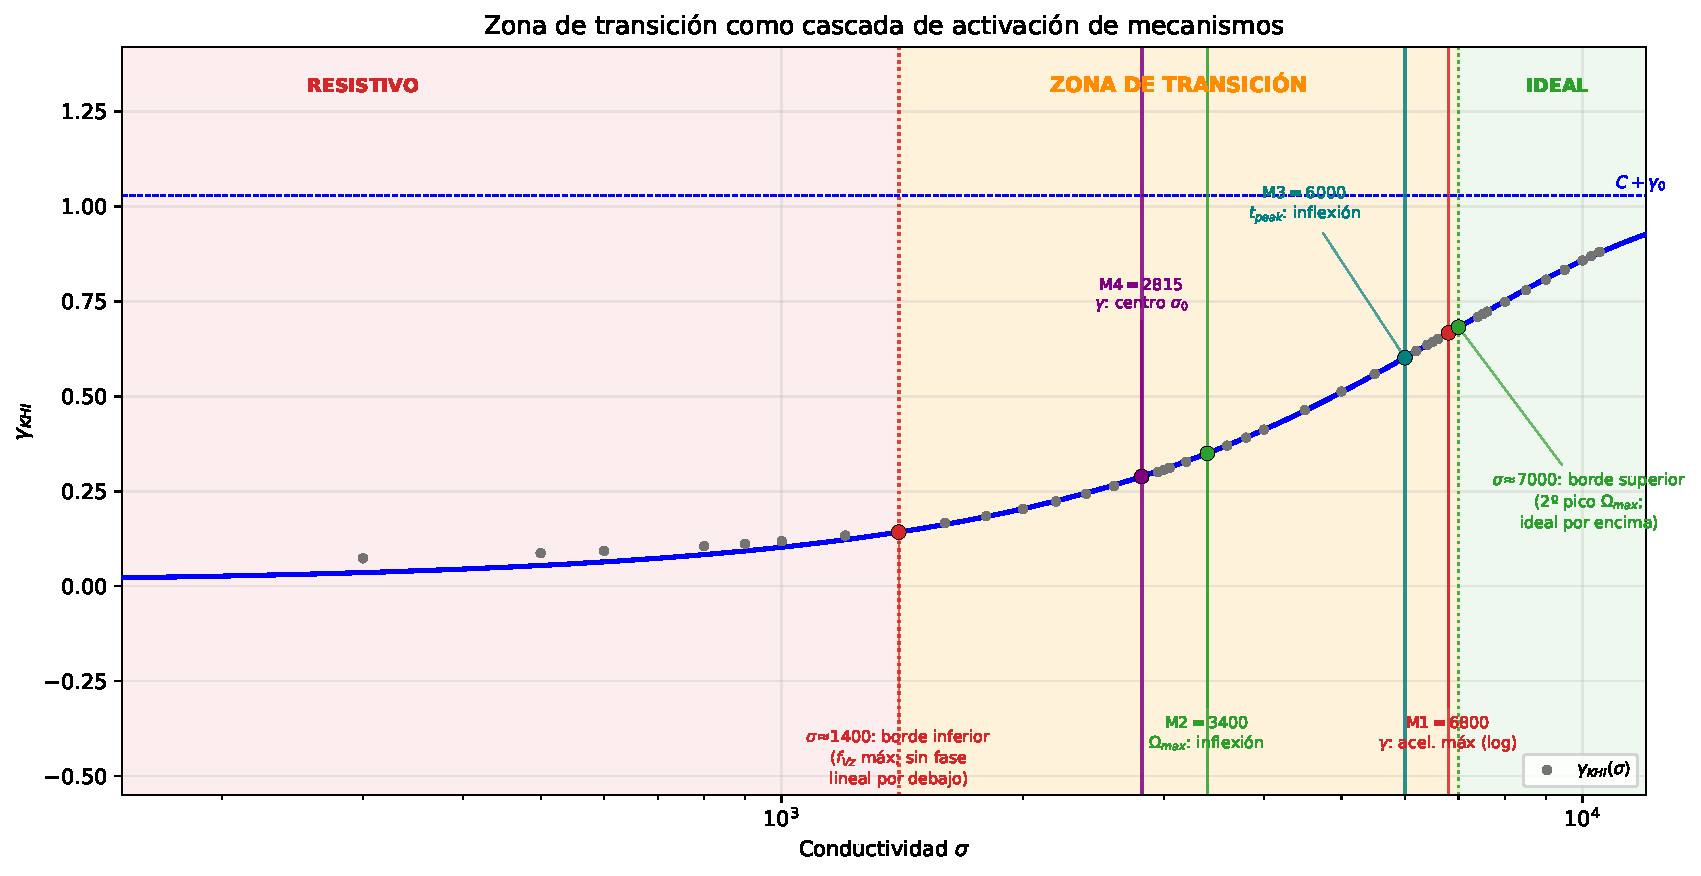
\includegraphics[width=\linewidth]{figures/fig_zona_transicion.pdf}
  \end{center}
\end{column}
\begin{column}{0.36\textwidth}
  \begin{block}{Lectura f\'isica}
    \scriptsize
    \begin{itemize}\setlength\itemsep{2pt}
      \item Cuatro estimadores independientes:
            $\sigma_0{=}2815$ (lineal), $3400$ ($\Omega^{\max}$),
            $6000$ ($t_{\rm peak}$), $6800$ ($\gamma$ log).
      \item Bordes le\'idos de los datos:
            $f_{Vz}$ m\'aximo ($\sigma\approx1400$) y saturaci\'on
            no lineal ($\sigma\approx7000$).
      \item Resultado: \textbf{zona} $\sigma\in[1400,7000]$,
            centro $\approx2815$; en Lundquist $S\sim10^3$.
    \end{itemize}
  \end{block}
  \begin{tcolorbox}[HYP={Mensaje epistemol\'ogico}]
    \scriptsize
    La dispersi\'on inter-m\'etodo ($\pm1944$) \textbf{no es ruido}:
    es la firma de una transici\'on \emph{multi-escala}. Reportar la banda
    --- y no un falso valor \'unico con error formal $\pm123$ ---
    es lo riguroso.
  \end{tcolorbox}
\end{column}
\end{columns}
\end{frame}

%------------------------------------------------------------------------------
% S22 · CONTRASTE CON TEORÍA LINEAL
%------------------------------------------------------------------------------
\begin{frame}{Contraste con la Teor\'ia Lineal: la Escalera de Predicciones}
\framesubtitle{Techo de Michalke $\to$ predicci\'on RMHD compresible $\to$ valor medido}
\begin{columns}[T]
\begin{column}{0.56\textwidth}
  \begin{center}
    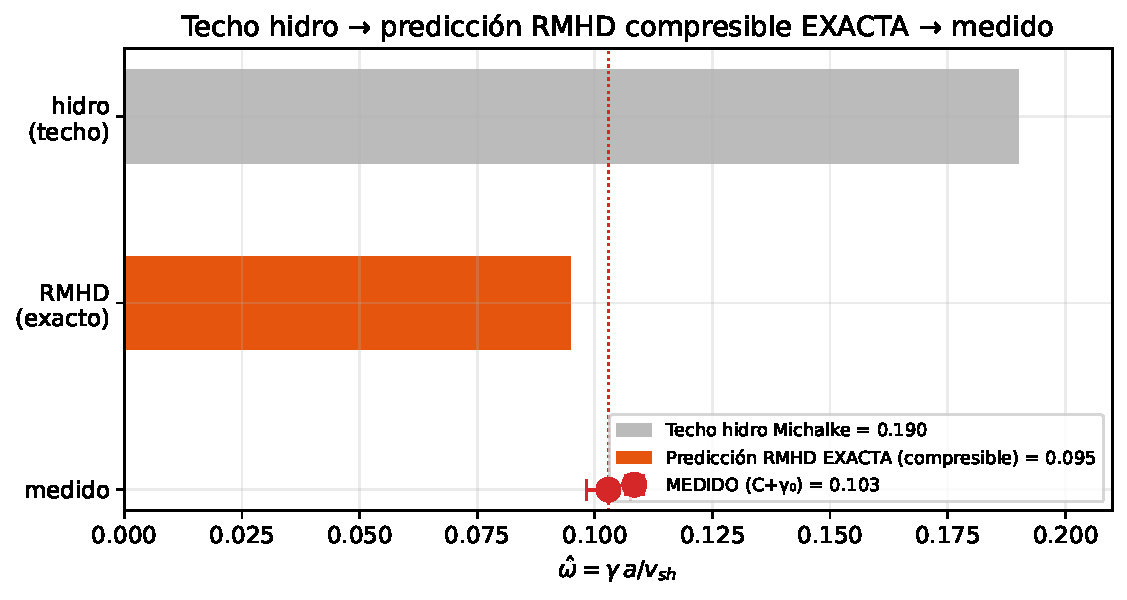
\includegraphics[width=0.94\linewidth]{figures/fig6_escalera.pdf}
  \end{center}
  \vspace{-0.08cm}
  \begin{tcolorbox}[RES={Acuerdo al 8\% sin par\'ametros de ajuste}]
    \scriptsize
    $\hat\omega_{\rm medido}=(C+\gamma_0)\,a_{kh}/v_{\rm sh}=0.103$
    \;vs.\; $\hat\omega_{\rm RMHD}=0.095$ (Lees--Lin compresible).\\
    Control negativo: con $c_s$ en vez de $v_{f\perp}$ el crecimiento
    colapsar\'ia a $\hat\omega\approx0.016$: \emph{es la presi\'on de $B_z$
    la que sostiene la inestabilidad}.
  \end{tcolorbox}
\end{column}
\begin{column}{0.42\textwidth}
  \begin{block}{La cadena l\'ogica}
    \scriptsize
    \begin{enumerate}\setlength\itemsep{2pt}
      \item \textbf{Techo inviscido}: Rayleigh para perfil $\tanh$;
            solver validado contra \citet{michalke1964}
            ($\hat\omega_{\max}=0.190$). \hfill{\tiny[resp.\ B6]}
      \item \textbf{Geometr\'ia fija la f\'isica}: $\mathbf k\perp\mathbf B$
            (campo gu\'ia) $\Rightarrow$ el campo aporta
            \emph{presi\'on pero no tensi\'on}: la velocidad de restituci\'on
            es la magnetos\'onica $v_{f\perp}=0.691$ \citep{chow2023}.
      \item \textbf{Criterio relativista}: $M_{re}=0.60<\sqrt2$
            \citep{konigl1980,bodo-2004}: holgadamente inestable.
    \end{enumerate}
  \end{block}
  \begin{tcolorbox}[WRN={Alcance del resultado (honestidad)}]
    \scriptsize
    Es una \textbf{consistencia cuantitativa fuerte}, no una validaci\'on
    cerrada: la as\'intota es extrapolaci\'on (el dato m\'aximo alcanza el
    $85\%$) y la predicci\'on usa $c_s\to v_{f\perp}$, no la dispersi\'on
    RMHD completa de grado 8.
  \end{tcolorbox}
\end{column}
\end{columns}
\end{frame}

%------------------------------------------------------------------------------
% S23 · LEY DE POTENCIA
%------------------------------------------------------------------------------
\begin{frame}{No Linealidad: Ley de Potencia de la Enstrof\'ia M\'axima}
\framesubtitle{Objetivo 2 --- $\Omega_{zp}^{\max}\propto\sigma^{1.22}$ excede el piso de una l\'amina \'unica}
\begin{columns}[T]
\begin{column}{0.58\textwidth}
  \begin{center}
    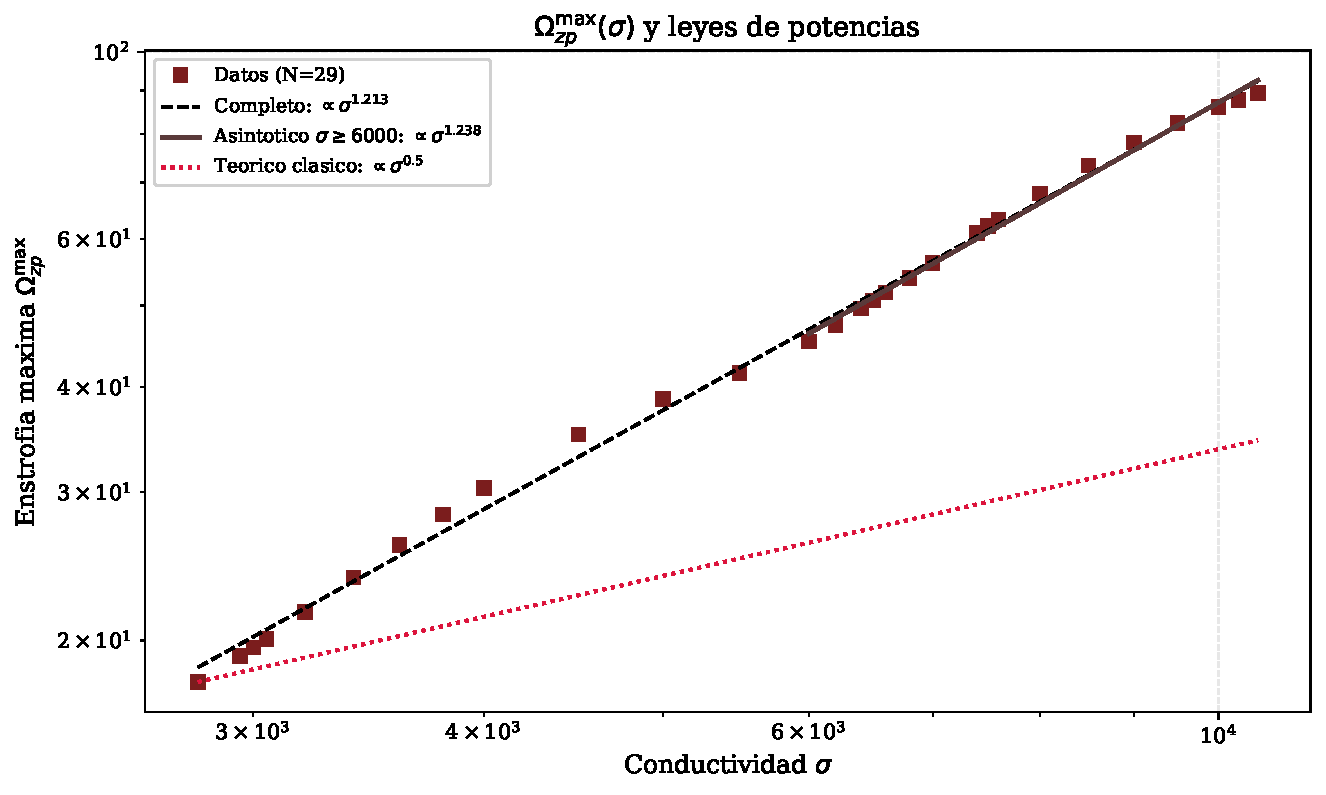
\includegraphics[width=\linewidth]{figures/fig_omega_max_leypotencias.pdf}
  \end{center}
\end{column}
\begin{column}{0.40\textwidth}
  \begin{block}{El piso te\'orico}
    \scriptsize
    Una l\'amina de corriente \textbf{Sweet--Parker \'unica}
    ($\delta\propto S^{-1/2}$, \citealp{parker1957}) dar\'ia
    $\Omega^{\max}\propto\sigma^{1/2}$; el escalamiento del espesor es
    robusto frente a correcciones relativistas \citep{lyubarsky2005}.
  \end{block}
  \begin{tcolorbox}[HYP={Interpretaci\'on (declarada como hip\'otesis)}]
    \scriptsize
    El exceso ($\alpha\approx1.22$, factor $\sim2.4$) sugiere que la
    l\'amina primaria se \textbf{fragmenta} (modo \textit{tearing},
    \citealp{furth1963}) multiplicando la superficie disipativa.
    Firma fenomenol\'ogica consistente con \citet{nastro2022};
    su derivaci\'on cuantitativa exige resolver la jerarqu\'ia de
    sub-l\'aminas (esquemas de 4.º orden, \citealp{mignone2024})
    $\Rightarrow$ trabajo futuro.
  \end{tcolorbox}
\end{column}
\end{columns}
\end{frame}

%------------------------------------------------------------------------------
% S24 · VARIABLES GLOBALES + BLINDAJE
%------------------------------------------------------------------------------
\begin{frame}{Variables Globales: la Firma Electromagn\'etica de $\sigma$}
\framesubtitle{Objetivo 3 --- y la evidencia de que la disipaci\'on es f\'isica, no num\'erica}
\begin{center}
  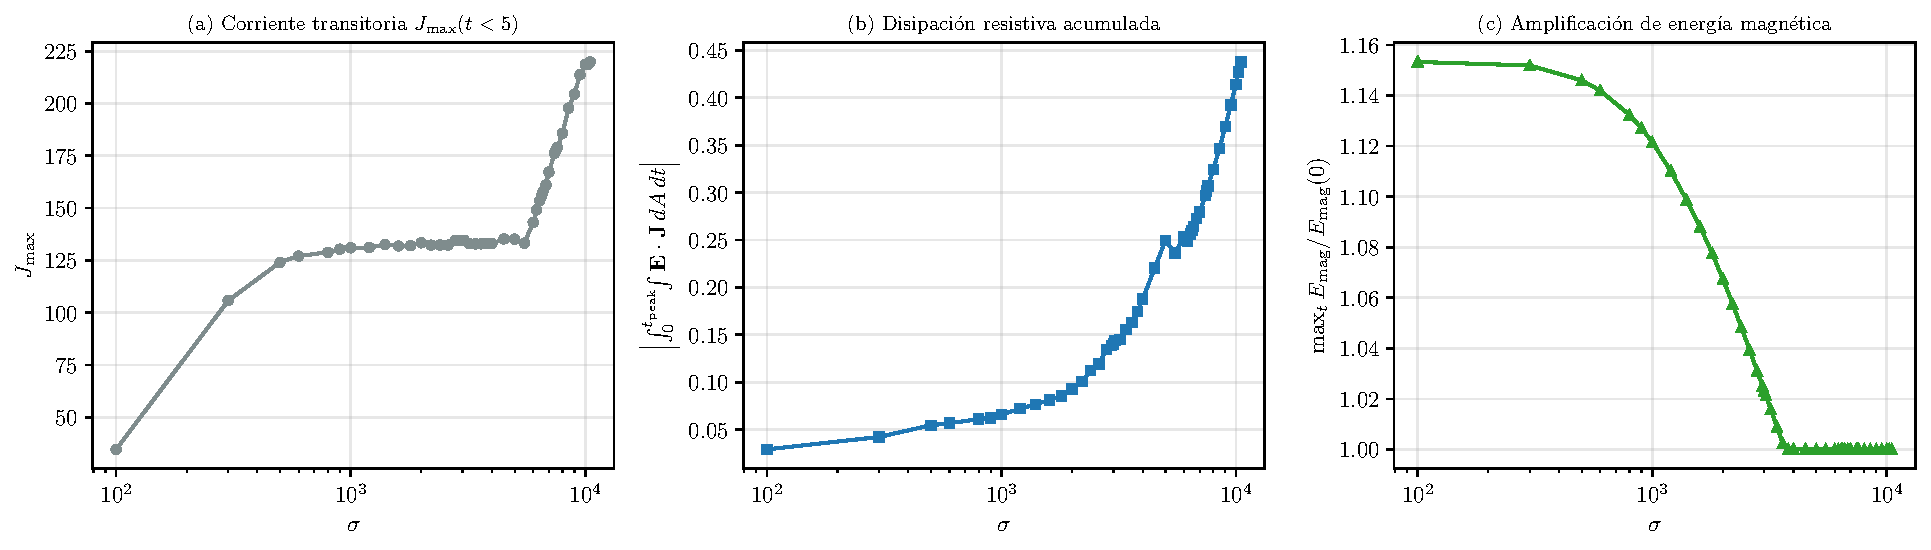
\includegraphics[width=0.9\textwidth]{figures/fig_global_campos_transitorio.pdf}
\end{center}
\vspace{-0.12cm}
\begin{columns}[T]
\begin{column}{0.55\textwidth}
  {\scriptsize
  \begin{itemize}\setlength\itemsep{1pt}
    \item \textbf{(b)} Trabajo EM disipado acumulado: crece $0.03\to0.44$
          --- a mayor $\sigma$, m\'as violencia hidrodin\'amica procesa
          m\'as energ\'ia magn\'etica.
    \item \textbf{(c)} Amplificaci\'on de $E_{\rm mag}$ propia:
          $\sim15\%\to0$ --- el congelamiento ideal impide reorganizar
          la topolog\'ia.
    \item $f_{Vz}$ (estructuras fuera del plano): m\'aximo $0.37$ en
          $\sigma\approx1400$, suprimidas en el ideal. {\tiny[resp.\ B13]}
  \end{itemize}}
\end{column}
\begin{column}{0.43\textwidth}
  \begin{tcolorbox}[RES={Blindaje num\'erico emp\'irico --- panel (a)}]
    \scriptsize
    El \textbf{plateau de $J_{\max}$} marca d\'onde la difusividad
    \emph{f\'isica} supera el error de truncamiento de la malla:
    los resultados en $\sigma\in[1400,7000]$ no est\'an contaminados por
    disipaci\'on artificial. Adem\'as, la KHI 2D \emph{ideal} no converge
    \citep{lecoanet2016}: la $\eta$ expl\'icita es la que da significado
    convergente a $\gamma_{\rm KHI}(\sigma)$ (buen planteamiento).
  \end{tcolorbox}
\end{column}
\end{columns}
\end{frame}

%==============================================================================
\section{Resultados II: campa\~na magn\'etica}
%==============================================================================

%------------------------------------------------------------------------------
% S25 · CAMPAÑA MAGNÉTICA I
%------------------------------------------------------------------------------
\begin{frame}{Campa\~na Magn\'etica I: Intensidad y Orientaci\'on}
\framesubtitle{Objetivo 4 --- qui\'en suprime: ?`presi\'on o tensi\'on?}
\begin{columns}[T]
\begin{column}{0.50\textwidth}
  \begin{center}
    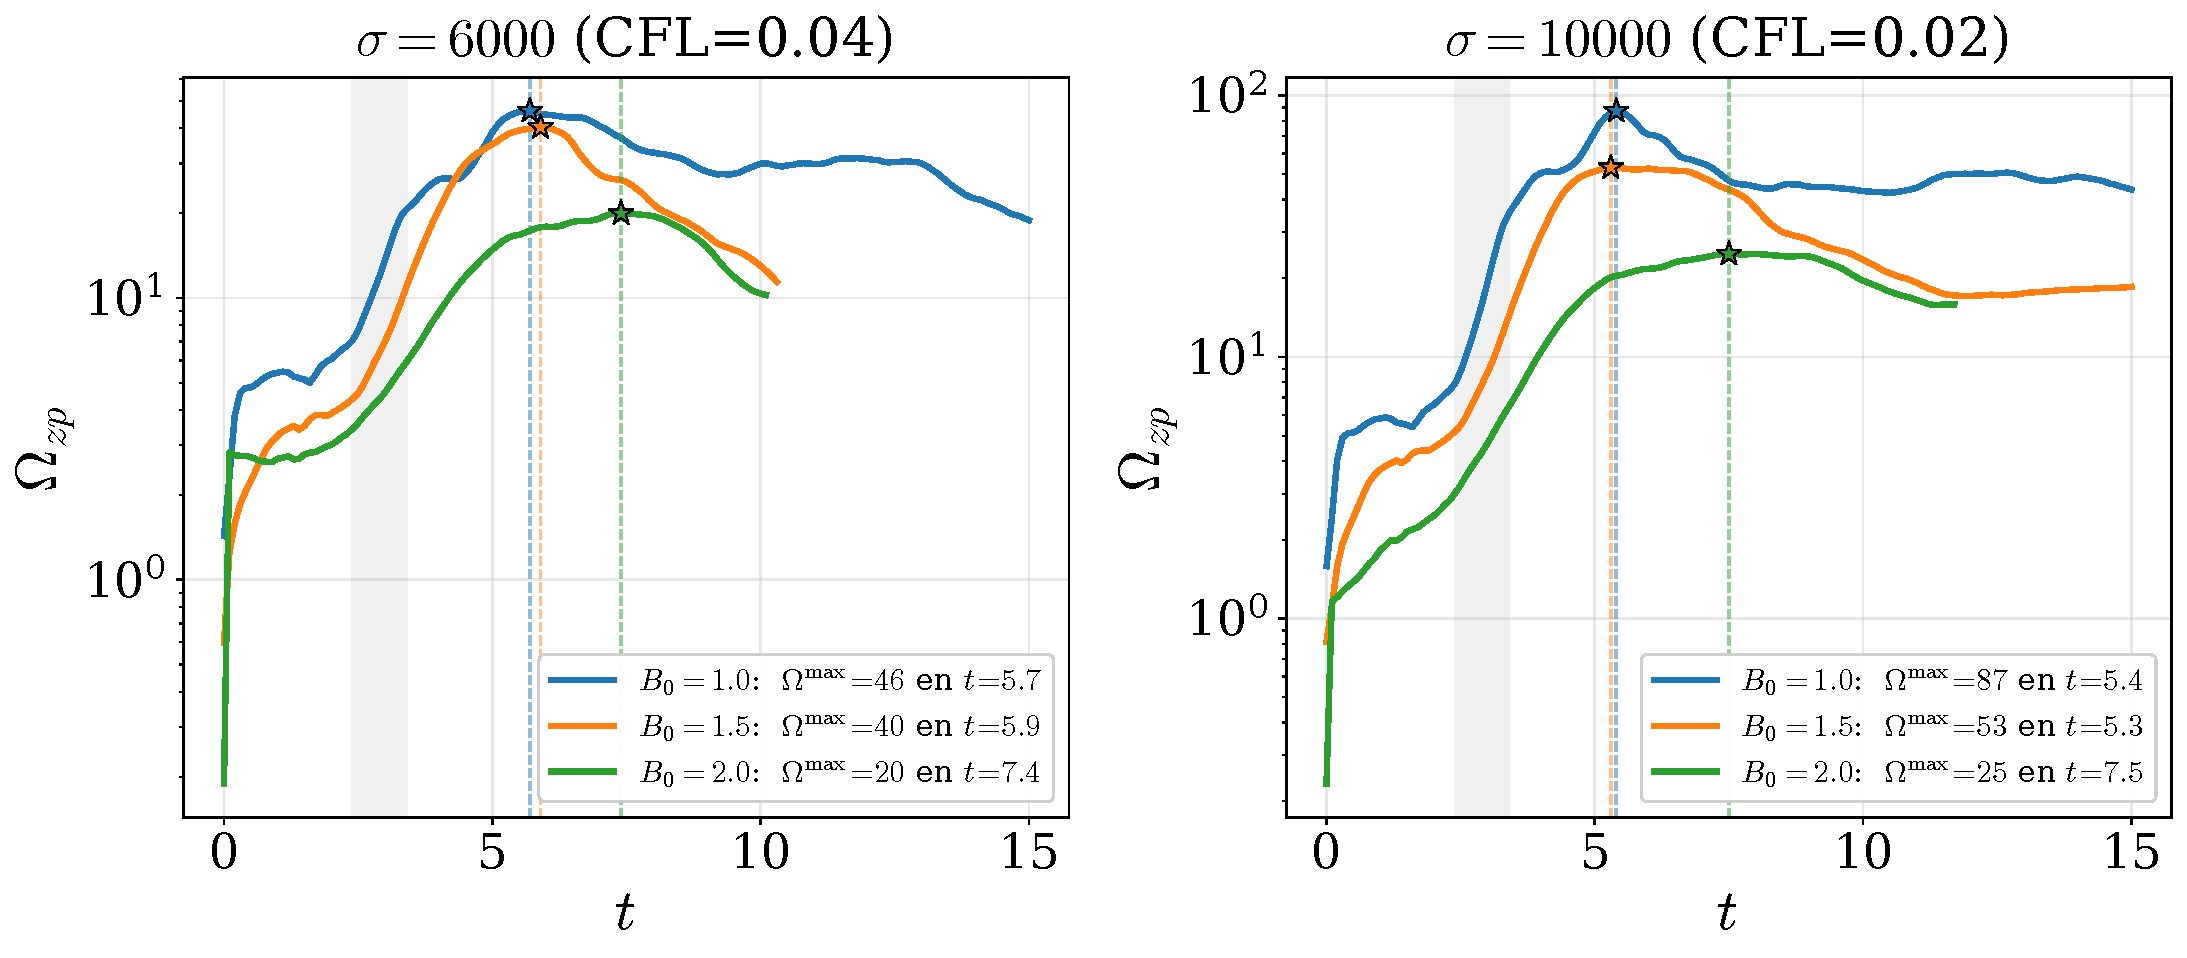
\includegraphics[width=\linewidth]{figures/fig_campA_enstrofia_slide.pdf}
  \end{center}
  \vspace{-0.1cm}
  \begin{tcolorbox}[RES={A --- Intensidad: suprime la \emph{presi\'on}}]
    \scriptsize
    Al subir $B_0$: $\gamma_{\rm KHI}$ cae $0.81\to0.38$ y
    $\Omega^{\max}_{zp}$ de $87\to25$ ($\sigma=10^4$). El flujo permanece
    \textbf{super-Alfv\'enico} paralelo ($M_{A,\parallel}=9.4\to6.4$):
    la tensi\'on es incapaz de frenar la cizalla
    $\Rightarrow$ el agente es la presi\'on magn\'etica / magnetizaci\'on
    ($\beta\propto B_0^{-2}$: $0.99\to0.25$).
  \end{tcolorbox}
\end{column}
\begin{column}{0.48\textwidth}
  \begin{center}
    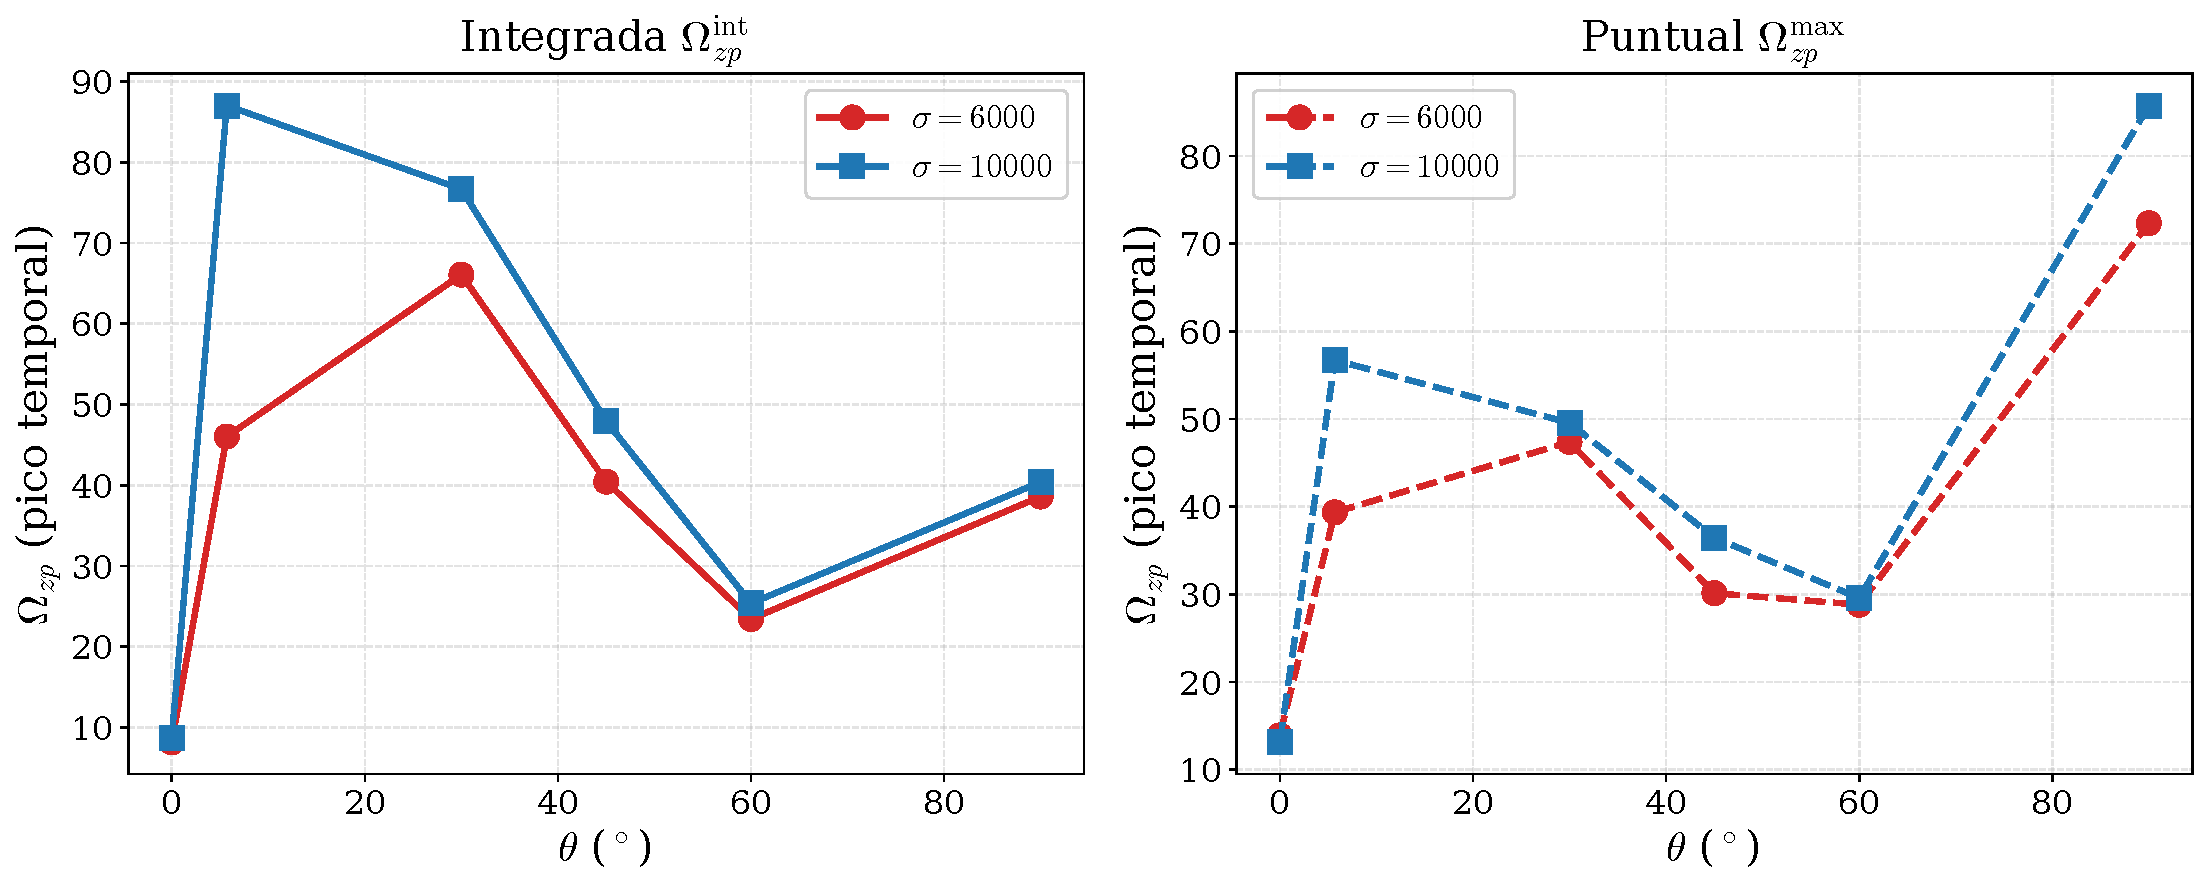
\includegraphics[width=\linewidth]{figures/fig_campB_omegamax_theta_slide.pdf}
  \end{center}
  \vspace{-0.1cm}
  \begin{tcolorbox}[HYP={B --- Orientaci\'on: la tensi\'on la ejerce solo $B_y\parallel\mathbf k$}]
    \scriptsize
    \textbf{Paradoja de $\theta=0^\circ$} (gu\'ia pura, sin tensi\'on,
    pero enstrof\'ia mínima): sin $B_y$ el v\'ortice 2D \emph{no puede}
    estirar l\'ineas en el plano $\Rightarrow$ sin d\'inamo ni reconexi\'on
    que realimenten \citep{mizuno-2013}. En $\theta=90^\circ$ el m\'aximo
    \emph{local} viene de capas de reconexi\'on finas: la integrada
    s\'i decrece con la tensi\'on --- efecto del observable, no de la f\'isica.
  \end{tcolorbox}
\end{column}
\end{columns}
\end{frame}

%------------------------------------------------------------------------------
% S26 · CAMPAÑA MAGNÉTICA II — BALANCE ENERGÉTICO
%------------------------------------------------------------------------------
\begin{frame}{Campa\~na Magn\'etica II: Balance Energ\'etico y Canales de Disipaci\'on}
\framesubtitle{Cuando la geometr\'ia enmascara la fase lineal, el observable es la energ\'ia}
\begin{center}
  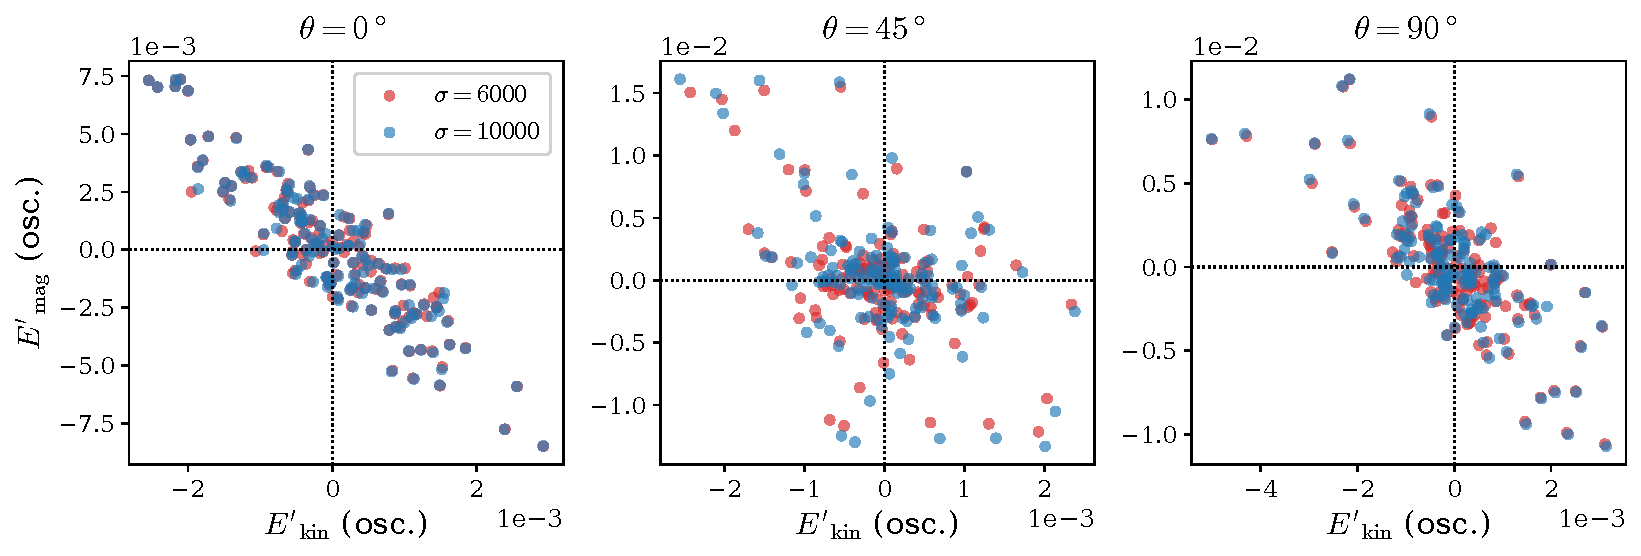
\includegraphics[width=0.72\textwidth]{figures/fig_campB_ekin_emag_scatter_slide.pdf}\\
  {\tiny\color{INF3} Parte oscilatoria de $E_{\rm kin}$ vs.\ $E_{\rm mag}$
   ($\theta=0^\circ,45^\circ,90^\circ$): anti-correlaci\'on
   $r\simeq-0.6$ a $-0.9$ (Campa\~na B; 6 \'angulos en la monograf\'ia).}
\end{center}
\vspace{-0.3cm}
\begin{columns}[T]
\begin{column}{0.58\textwidth}
  \begin{block}{Tres hallazgos}
    \scriptsize
    \begin{itemize}\setlength\itemsep{2pt}
      \item $E_{\rm kin}\leftrightarrow E_{\rm mag}$ oscilan en
            \textbf{anti-fase} ciclo a ciclo: canal de conversi\'on
            directo y reversible (d\'inamo $\leftrightarrow$ rebote
            el\'astico de la tensi\'on).
      \item \textbf{La resistividad fija el destino de la energ\'ia}:
            a $\sigma=10^4$ intercambio cuasi-reversible; a $\sigma=6000$
            la disipaci\'on \'ohmica desv\'ia energ\'ia a calor
            (a $\theta=90^\circ$, hasta un orden de magnitud m\'as).
      \item Sin tensi\'on (Campa\~na C): conversi\'on casi uno a uno
            ($r\approx-0.98$) y disipaci\'on mon\'otona con $\theta$.
    \end{itemize}
  \end{block}
\end{column}
\begin{column}{0.40\textwidth}
  \begin{tcolorbox}[RES={Control de calidad interno}]
    \scriptsize
    Conservaci\'on de $E_{\rm tot}$ con error relativo $\lesssim10^{-3}$
    en todas las corridas: validaci\'on independiente del esquema.
  \end{tcolorbox}
\end{column}
\end{columns}
\end{frame}

%------------------------------------------------------------------------------
% S27 · CAMPAÑA MAGNÉTICA III — CAMPAÑA C (SIN TENSIÓN)
%------------------------------------------------------------------------------
\begin{frame}{Campa\~na Magn\'etica III: Orientaci\'on sin Tensi\'on (plano $x$--$z$)}
\framesubtitle{El experimento de control: $B_y=0$ elimina la tensi\'on sobre el v\'ortice}
\begin{columns}[T]
\begin{column}{0.52\textwidth}
  \begin{center}
    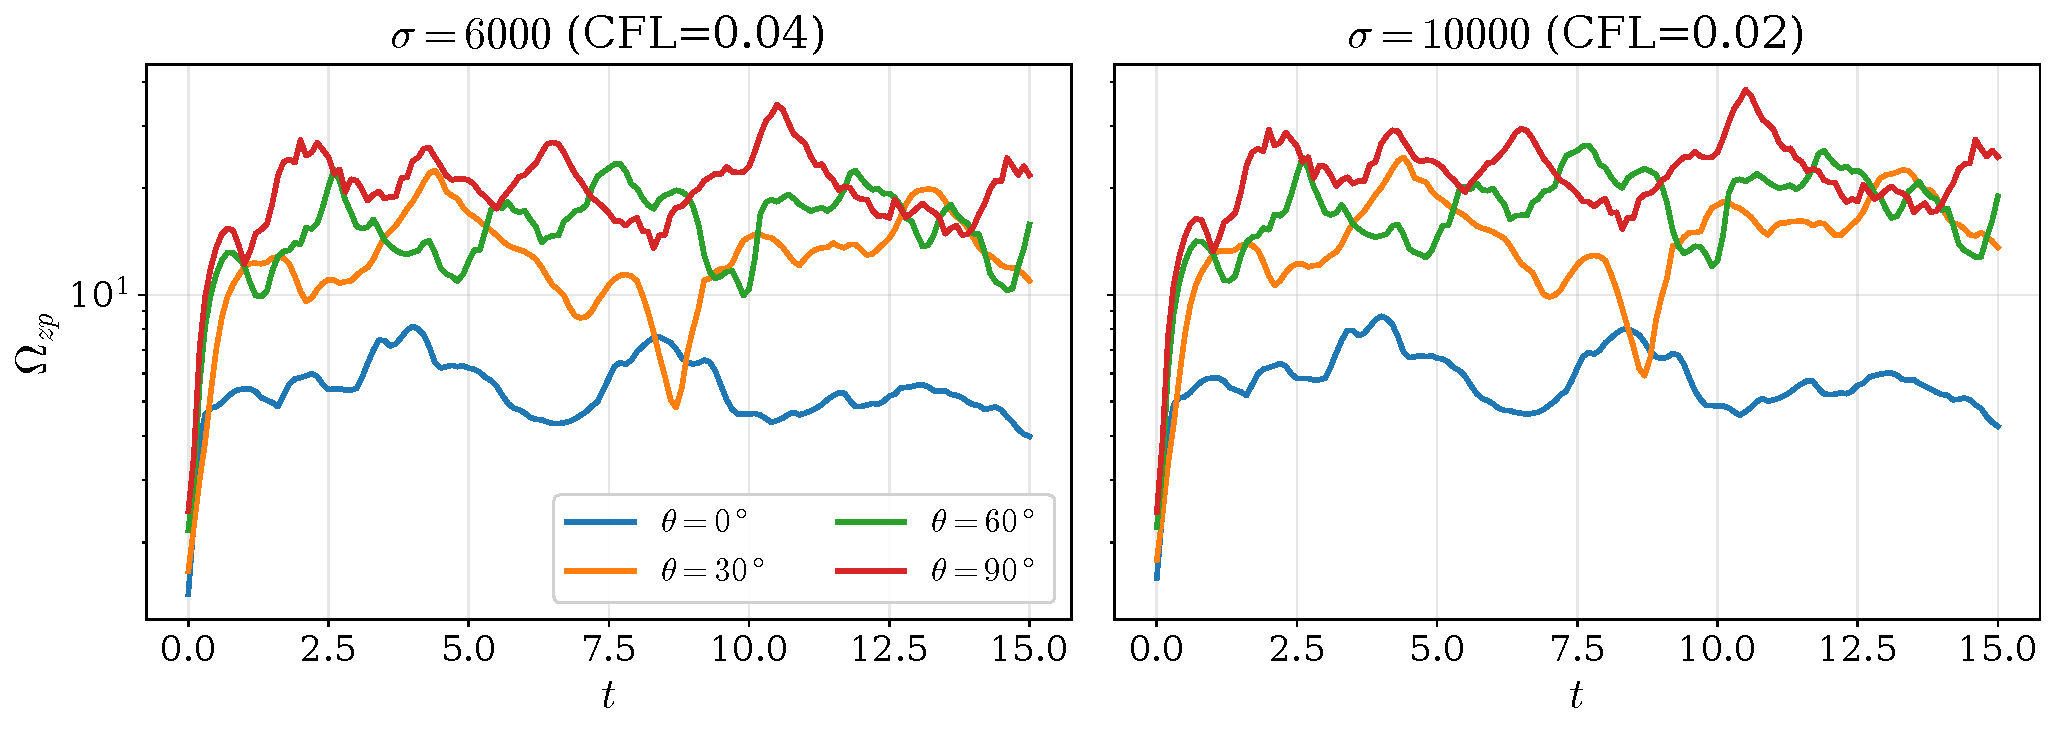
\includegraphics[height=0.55\textheight]{figures/fig_campC_enstrofia_slide.pdf}
  \end{center}
  \vspace{-0.2cm}
  \begin{tcolorbox}[WRN={C --- sin tensi\'on no hay fase lineal limpia}]
    \scriptsize
    $|\mathbf B|$ ---y la presi\'on magn\'etica--- es constante con
    $\theta$: la fenomenolog\'ia es puramente geom\'etrica
    (reorientaci\'on de $B_x$; topolog\'ia de reconexi\'on). Sin $B_y$
    que soporte el v\'ortice, el crecimiento pierde la fase exponencial
    y la mezcla se vuelve difusa --- id\'entico en ambas $\sigma$
    $\Rightarrow$ \textbf{la tensi\'on es el estabilizador primario}.
  \end{tcolorbox}
\end{column}
\begin{column}{0.44\textwidth}
  \begin{center}
    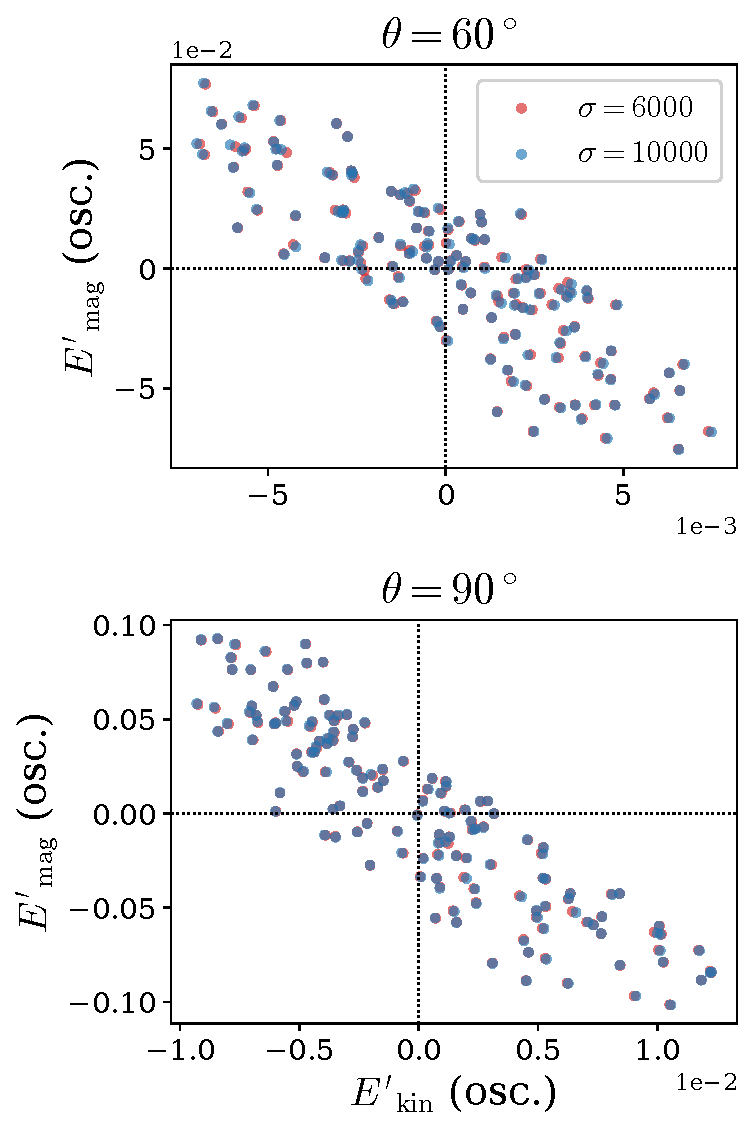
\includegraphics[height=0.55\textheight]{figures/fig_campC_ekin_emag_scatter_slide.pdf}
  \end{center}
  \vspace{-0.2cm}
  \begin{tcolorbox}[RES={La conversi\'on queda al desnudo}]
    \scriptsize
    Sin el intercambio guiado por la tensi\'on, la anti-correlaci\'on
    $E'_{\rm kin}$--$E'_{\rm mag}$ se intensifica con $\theta$ hasta
    $r\approx-0.98$ ($\theta=60^\circ$ y $90^\circ$): conversi\'on
    cin\'etico$\leftrightarrow$magn\'etica casi uno a uno; disipaci\'on
    \'ohmica mon\'otona con $\theta$.
  \end{tcolorbox}
\end{column}
\end{columns}
\end{frame}

%==============================================================================
\section{Conclusiones y perspectivas}
%==============================================================================

%------------------------------------------------------------------------------
% S27 · CONCLUSIONES
%------------------------------------------------------------------------------
\begin{frame}{Conclusiones (por objetivo)}
\begin{columns}[T]
\begin{column}{0.48\textwidth}
  \begin{tcolorbox}[EQ={1 · Tasa de crecimiento vs.\ resistividad}]
    \scriptsize
    Transici\'on resistivo$\to$ideal descrita por el sigmoide con
    \emph{offset}; as\'intota ideal $C+\gamma_0=1.03\pm0.05$
    ($\hat\omega=0.103$), consistente al $8\%$ con la teor\'ia lineal RMHD
    compresible. $\sigma_{\rm crit}$: \textbf{zona} $[1400,7000]$,
    centro $\approx2815$.
  \end{tcolorbox}
  \vspace{0.08cm}
  \begin{tcolorbox}[EQ={2 · Estructuras secundarias}]
    \scriptsize
    $\Omega^{\max}_{zp}\propto\sigma^{1.22}$: excede el piso Sweet--Parker
    ($\sigma^{1/2}$) $\Rightarrow$ firma de reconexi\'on resistiva,
    hip\'otesis de \textit{tearing} secundario. $f_{Vz}$ m\'aximo en la
    transici\'on: las estructuras 3D emergen donde difusi\'on y advecci\'on
    compiten.
  \end{tcolorbox}
\end{column}
\begin{column}{0.48\textwidth}
  \begin{tcolorbox}[EQ={3 · Variables globales}]
    \scriptsize
    La conductividad controla la intensidad de las l\'aminas de corriente
    ($J_{\max}$), la disipaci\'on acumulada (crece con $\sigma$) y la
    amplificaci\'on de la energ\'ia magn\'etica propia
    ($15\%\to0$ hacia el ideal).
  \end{tcolorbox}
  \vspace{0.08cm}
  \begin{tcolorbox}[EQ={4 · Intensidad y orientaci\'on de $\mathbf B$}]
    \scriptsize
    La supresi\'on por intensidad es de \textbf{presi\'on/magnetizaci\'on}
    (flujo super-Alfv\'enico); la \textbf{tensi\'on} solo act\'ua v\'ia
    $B_y\parallel\mathbf k$; sin tensi\'on domina la reconexi\'on.
    Anti-fase $E_{\rm kin}\leftrightarrow E_{\rm mag}$: la resistividad
    decide entre intercambio reversible y calor.
  \end{tcolorbox}
\end{column}
\end{columns}
\end{frame}

%------------------------------------------------------------------------------
% S28 · LIMITACIONES Y TRABAJO FUTURO
%------------------------------------------------------------------------------
\begin{frame}{Limitaciones del Modelo y Trabajo Futuro}
\framesubtitle{Los l\'imites se declaran: son el mapa del trabajo por venir}
\begin{columns}[T]
\begin{column}{0.50\textwidth}
  \begin{tcolorbox}[WRN={Limitaciones declaradas de antemano}]
    \scriptsize
    \begin{itemize}\setlength\itemsep{2pt}
      \item \textbf{2D}: suprime modos 3D y cascada turbulenta plena.
      \item \textbf{EoS politr\'opica} $\Gamma=4/3$: sin composici\'on
            ni radiaci\'on.
      \item \textbf{$\sigma$ escalar}: sin Hall ni anisotrop\'ia.
            El continuo unifluido trunca la jerarqu\'ia de momentos de
            Vlasov; v\'alido mientras la escala disipativa sea la capa
            resistiva $\delta\sim S^{-1/2}$, no el girorradio.
            \hfill{\tiny[resp.\ B11]}
      \item \textbf{Resoluci\'on}: a alta $\sigma$ las l\'aminas rozan
            el l\'imite de malla (condiciona el exponente $1.22$).
      \item \textbf{As\'intota ideal extrapolada}: el dato m\'aximo
            ($\sigma=10\,500$) alcanza el $85\%$ del plateau.
    \end{itemize}
  \end{tcolorbox}
\end{column}
\begin{column}{0.48\textwidth}
  \begin{tcolorbox}[RES={Trabajo futuro}]
    \scriptsize
    \begin{itemize}\setlength\itemsep{2pt}
      \item \textbf{Medir el plateau ideal}: 2--3 simulaciones a
            $\mathrm{Rm}^*\gtrsim500$ ($\sigma\sim2$--$3\times10^4$)
            para convertir la extrapolaci\'on en medici\'on.
      \item Resolver la \textbf{dispersi\'on RMHD completa} (grado 8;
            \citealp{osmanov-2008,chow2023}) en estos par\'ametros.
      \item \textbf{Mapa fino} de la frontera tensi\'on vs.\ presi\'on
            (m\'as \'angulos y conductividades).
      \item Extensi\'on \textbf{3D} y esquemas de \textbf{4.º orden}
            \citep{mignone2024} para resolver las hojas resistivas.
      \item A largo plazo: h\'ibridos fluido-cin\'eticos para la
            frontera no colisional.
    \end{itemize}
  \end{tcolorbox}
\end{column}
\end{columns}
\end{frame}

%------------------------------------------------------------------------------
% REFERENCIAS
%------------------------------------------------------------------------------
\begin{frame}[allowframebreaks]{Referencias}
\scriptsize
\bibliographystyle{unsrtnat}
\bibliography{references}
\end{frame}

%------------------------------------------------------------------------------
% S29 · GRACIAS
%------------------------------------------------------------------------------
{
\setbeamertemplate{footline}{}\setbeamertemplate{headline}{}
\begin{frame}[plain]
\begin{tikzpicture}[remember picture,overlay]
  \node[at=(current page.center),inner sep=0]
    {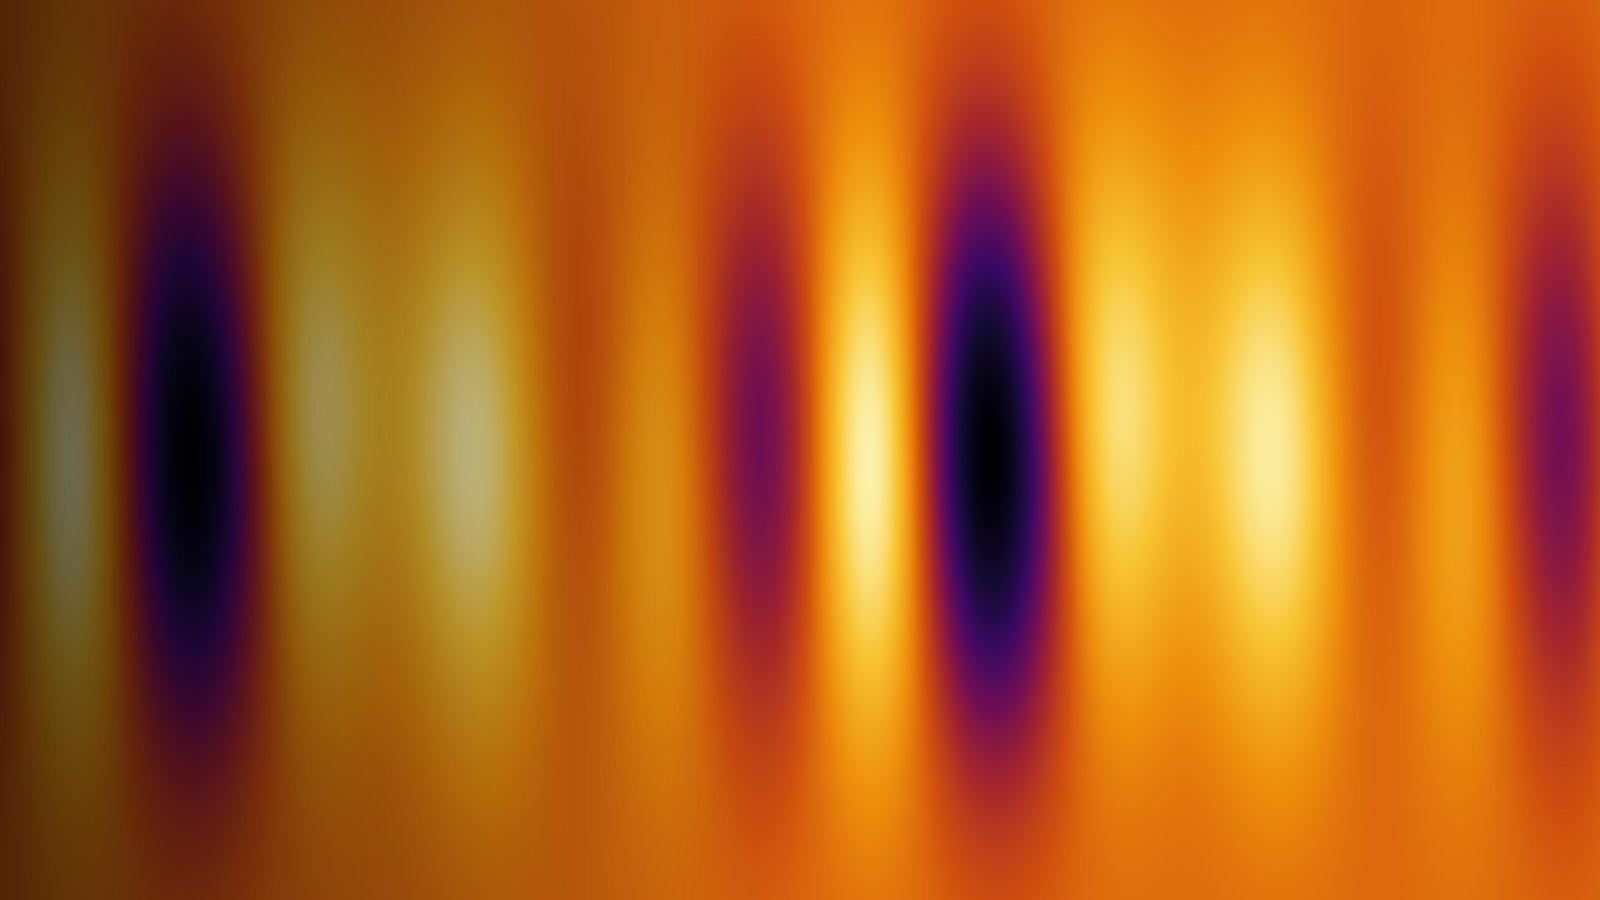
\includegraphics[width=\paperwidth,height=\paperheight,
       keepaspectratio=false]{figures/khi_simulation_bg.png}};
  \fill[primary,opacity=0.82]
    (current page.south west) rectangle (current page.north east);
  \shade[left color=brick,right color=INF7,opacity=1]
    (current page.south west)
    rectangle ([yshift=0.18\paperheight]current page.south east);
  \draw[soft!65,line width=1.2pt]
    ([yshift=0.18\paperheight]current page.south west)
    -- ([yshift=0.18\paperheight]current page.south east);
\end{tikzpicture}
\begin{center}
  \vspace{-0.15cm}
  {\color{gold}\Large$\bigstar$}\\[0.3cm]
  {\color{soft}\LARGE\bfseries !`Gracias por su Atenci\'on!}\\[0.4cm]
  {\color{accent}\rule{0.42\textwidth}{1pt}}\\[0.4cm]
  {\color{soft!80}\large Preguntas y Discusi\'on}\\[0.6cm]
  {\color{soft}\normalsize
    Bryan Martinez Anzola $\;\cdot\;$ Sebasti\'an Rodriguez Garcia}\\[0.15cm]
  {\color{soft!70}\small Director: Prof.\ Ph.D.\ Sergio Miranda-Aranguren}\\[0.3cm]
  {\color{soft!55}\small Universidad Distrital Francisco Jos\'e de Caldas}\\[0.15cm]
  {\color{soft!45}\footnotesize Bogot\'a, Julio de 2026}
\end{center}
\end{frame}
}

%==============================================================================
% MATERIAL DE RESPALDO
%==============================================================================
\appendix

{
\setbeamertemplate{footline}{}
\begin{frame}[plain]
\begin{tikzpicture}[remember picture,overlay]
  \fill[primary] (current page.south west) rectangle (current page.north east);
  \fill[accent]
    ([yshift=-0.47\paperheight]current page.north west)
    rectangle ([yshift=-0.50\paperheight]current page.north east);
\end{tikzpicture}
\begin{center}
  \vspace{1.6cm}
  {\color{soft}\LARGE\bfseries Material de Respaldo}\\[0.5cm]
  {\color{gold}\small B1--B14: derivaciones, validaciones y an\'alisis complementarios}
\end{center}
\end{frame}
}

%------------------------------------------------------------------------------
% B1 · F=dA Y BIANCHI
%------------------------------------------------------------------------------
\begin{frame}{B1 · El Tensor de Faraday desde el Cuadripotencial}
\begin{columns}[T]
\begin{column}{0.50\textwidth}
  \begin{tcolorbox}[EQ={La 2-forma de Faraday e invariancia de gauge}]
    \scriptsize
    $A=A_\mu dx^\mu$ (1-forma). Gauge: $A\to A+d\Lambda$. Entonces
    \[
      dA'=dA+d(d\Lambda)=dA \quad (d^2=0)
    \]
    \[
      F\equiv dA=\tfrac12(\partial_\mu A_\nu-\partial_\nu A_\mu)\,
        dx^\mu\!\wedge dx^\nu
    \]
    \[
      \Rightarrow\quad F_{\mu\nu}=\partial_\mu A_\nu-\partial_\nu A_\mu
    \]
    Los observables: $\mathbf E=-\nabla\phi-\partial_t\mathbf A$,\;
    $\mathbf B=\nabla\times\mathbf A$.
  \end{tcolorbox}
\end{column}
\begin{column}{0.46\textwidth}
  \begin{tcolorbox}[RES={Identidad de Bianchi $\equiv$ par homog\'eneo}]
    \scriptsize
    \[
      dF=d(dA)=d^2A=0
      \;\Longleftrightarrow\;
      \partial_\mu(\star F)^{\mu\nu}=0
    \]
    Contiene $\nabla\!\cdot\!\mathbf B=0$ y Faraday--Lenz.
    Es \textbf{topolog\'ia} (consecuencia de definir $F$ desde un
    potencial), no din\'amica. La din\'amica est\'a en
    $\partial_\mu F^{\mu\nu}=J^\nu$ (m\'inima acci\'on), cuya divergencia
    da autom\'aticamente $\partial_\nu J^\nu=0$ (antisimetr\'ia).
  \end{tcolorbox}
  \vspace{0.1cm}
  {\scriptsize\color{INF3} Nota: $d(dx^\nu)=d^2x^\nu=0$ es leg\'itimo ---
  no es una segunda derivada del c\'alculo sino $d$ aplicado dos veces
  (nilpotencia).}
\end{column}
\end{columns}
\end{frame}

%------------------------------------------------------------------------------
% B2 · HILBERT
%------------------------------------------------------------------------------
\begin{frame}{B2 · Tensor de Energ\'ia-Momento por Derivada Funcional de Hilbert}
\begin{columns}[T]
\begin{column}{0.50\textwidth}
  \begin{tcolorbox}[EQ={Definici\'on variacional}]
    \scriptsize
    \[
      T^{\mu\nu}=-\frac{2}{\sqrt{-g}}\frac{\delta S}{\delta g_{\mu\nu}},
      \qquad S=S_{\rm em}+S_{\rm fluid}
    \]
    \[
      S_{\rm em}=\int\!\Bigl(-\tfrac14F_{\alpha\beta}F_{\gamma\delta}
        g^{\alpha\gamma}g^{\beta\delta}\Bigr)\sqrt{-g}\,d^4x
      \;\Rightarrow\;
      T^{\mu\nu}_{\rm em}
    \]
    \[
      S_{\rm fluid}=\int p\,\sqrt{-g}\,d^4x\ \text{(Taub)}
      \;\Rightarrow\;
      T^{\mu\nu}_{\rm fluid}=\rho h\,u^\mu u^\nu+p\,\eta^{\mu\nu}
    \]
  \end{tcolorbox}
\end{column}
\begin{column}{0.46\textwidth}
  \begin{block}{Dos preguntas t\'ipicas}
    \scriptsize
    \begin{itemize}\setlength\itemsep{3pt}
      \item \emph{?`Por qu\'e $S_{\rm em}$ no incluye $J_\mu A^\mu$?}
            El t\'ermino de fuente no depende de $g_{\mu\nu}$
            $\Rightarrow$ no contribuye a la variaci\'on m\'etrica;
            el acople aparece en la din\'amica (variaci\'on en $A_\nu$).
      \item \emph{?`La acci\'on de fluido perfecto vale en RRMHD?}
            S\'i: la disipaci\'on reside en el \textbf{sector
            electromagn\'etico} (Ohm con $\sigma$ finita), no en
            $T^{\mu\nu}_{\rm fluid}$ --- el fluido sigue siendo perfecto.
    \end{itemize}
  \end{block}
  \vspace{0.08cm}
  {\scriptsize Intercambio energ\'etico:
   $\partial_\mu T^{\mu\nu}_{\rm em}=-F^{\nu\lambda}J_\lambda$
   $\Rightarrow$ $\partial_\mu T^{\mu\nu}_{\rm fluid}=+F^{\nu\lambda}J_\lambda$
   (fuerza de Lorentz covariante).}
\end{column}
\end{columns}
\end{frame}

%------------------------------------------------------------------------------
% B3 · TELÉGRAFO VS DEDNER
%------------------------------------------------------------------------------
\begin{frame}{B3 · GLM: de la Acci\'on Extendida a la Forma de Dedner}
\begin{columns}[T]
\begin{column}{0.50\textwidth}
  \begin{tcolorbox}[EQ={Acci\'on extendida (sector el\'ectrico)}]
    \scriptsize
    \[
      S=\!\int\! d^4x\Bigl[-\tfrac14F^2+J_\mu A^\mu
        +\tfrac12\partial_\mu\Phi\,\partial^\mu\Phi
        -\Phi\,\partial_\mu A^\mu\Bigr]
    \]
    \[
      \delta A:\ \partial_\mu F^{\mu\nu}+\partial^\nu\Phi=J^\nu;
      \qquad
      \delta\Phi:\ \Box\Phi=-\partial_\mu A^\mu
    \]
    Disipaci\'on covariante: $\kappa\,n^\mu\partial_\mu\Phi$
    (fricci\'on a lo largo del observador euleriano)
    $\Rightarrow$ ecuaci\'on del tel\'egrafo. An\'alogo formal al
    mecanismo de Stueckelberg \citep{lee2004}.
  \end{tcolorbox}
\end{column}
\begin{column}{0.46\textwidth}
  \begin{tcolorbox}[RES={Por qu\'e el c\'odigo integra el 1.er orden}]
    \scriptsize
    Sistema 3+1 (forma de Dedner), equivalente al tel\'egrafo en el
    l\'imite continuo \citep{Dedner-2002}:
    \begin{itemize}\setlength\itemsep{2pt}
      \item El solucionador de Riemann exige la forma matricial
            hiperb\'olica de 1.er orden;
      \item permite acoplar los t\'erminos no conservativos de
            \textbf{Godunov--Powell};
      \item devela el modelo como sistema SHTC
            (termodin\'amicamente compatible).
    \end{itemize}
    Velocidad de limpieza $c_h=1$: el error viaja al cono causal m\'aximo.
  \end{tcolorbox}
\end{column}
\end{columns}
\end{frame}

%------------------------------------------------------------------------------
% B4 · ESPECTRO Y CFL
%------------------------------------------------------------------------------
\begin{frame}{B4 · Espectro Caracter\'istico y Estabilidad Temporal}
\begin{columns}[T]
\begin{column}{0.50\textwidth}
  \begin{tcolorbox}[EQ={Los 14 autovalores \citep{miranda-aranguren-2018}}]
    \scriptsize
    \begin{itemize}\setlength\itemsep{2pt}
      \item $\lambda^\pm_{EB}=\pm c$ ($\times8$): ondas EM $+$ modos
            de limpieza GLM.
      \item $\lambda_f^\pm$: magnetos\'onicas r\'apidas (sector fluido).
      \item $\lambda_c=v_x$ ($\times3$): entrop\'ia $+$ cizalla
            (discontinuidad de contacto).
      \item $\lambda_q=v_x$: onda de carga.
    \end{itemize}
    En el l\'imite ideal reaparecen Alfv\'en y lentas; con $W\to\infty$
    todo el espectro colapsa al cono de luz (degeneraci\'on
    ultrarrelativista).
  \end{tcolorbox}
\end{column}
\begin{column}{0.46\textwidth}
  \begin{tcolorbox}[RES={Condici\'on subcaracter\'istica y CFL}]
    \scriptsize
    Sistema hiperb\'olico con relajaci\'on: estabilidad causal si
    $|\lambda_{\rm RRMHD}|\le|\lambda_{\rm MHD}|\le c$ (Liu 1987).\\[3pt]
    CFL conservador ($0.1$; $0.04$/$0.02$ en campo fuerte) por la rigidez
    de la fuente resistiva y la agudeza de las l\'aminas de corriente
    --- el paso temporal queda dominado por la advecci\'on
    ($\Delta t\propto\Delta x$), no por $\sigma$.
  \end{tcolorbox}
\end{column}
\end{columns}
\end{frame}

%------------------------------------------------------------------------------
% B5 · OHM 3+1 COMPLETA
%------------------------------------------------------------------------------
\begin{frame}{B5 · Proyecci\'on 3+1 de la Ley de Ohm --- \'Algebra Completa}
\begin{columns}[T]
\begin{column}{0.52\textwidth}
  \begin{tcolorbox}[EQ={Descomposici\'on ortogonal de $J^\mu$}]
    \scriptsize
    $J^\mu=\rho_e u^\mu+j^\mu$, con $\rho_e=-J^\nu u_\nu$ (carga propia)
    y $j^\mu=h^\mu_{\ \nu}J^\nu$ (conducci\'on, $j^\mu u_\mu=0$).\\[2pt]
    Con $u^\mu=(W,W\mathbf v)$ y $E^\mu=F^{\mu\nu}u_\nu$:
    \[
      \mu=0:\ \rho_q=\rho_eW+\sigma W(\mathbf E\cdot\mathbf v)
    \]
    \[
      \mu=i:\ \mathbf J=\rho_eW\mathbf v
        +\sigma W(\mathbf E+\mathbf v\times\mathbf B)
    \]
    Eliminando $\rho_e$ entre ambas:
    \[
      \mathbf J=\rho_q\mathbf v+\sigma W\bigl[\mathbf E
        +\mathbf v\times\mathbf B-(\mathbf E\cdot\mathbf v)\mathbf v\bigr]
    \]
  \end{tcolorbox}
\end{column}
\begin{column}{0.44\textwidth}
  \begin{center}
    
\includegraphics[width=\linewidth]{figures/marco_comovil_lab.pdf}\\[2pt]
    {\tiny\color{INF3} $\rho_e$ (com\'ovil, rebanada ortogonal a $u^\mu$)
     vs.\ $\rho_q$ (laboratorio, $t=$ cte): coinciden solo si el fluido
     est\'a en reposo respecto a la malla.}
  \end{center}
\end{column}
\end{columns}
\end{frame}

%------------------------------------------------------------------------------
% B6 · VALIDACIÓN DEL SOLVER LINEAL
%------------------------------------------------------------------------------
\begin{frame}{B6 · Validaci\'on del Solucionador de la Teor\'ia Lineal}
\begin{columns}[T]
\begin{column}{0.48\textwidth}
  \begin{center}
    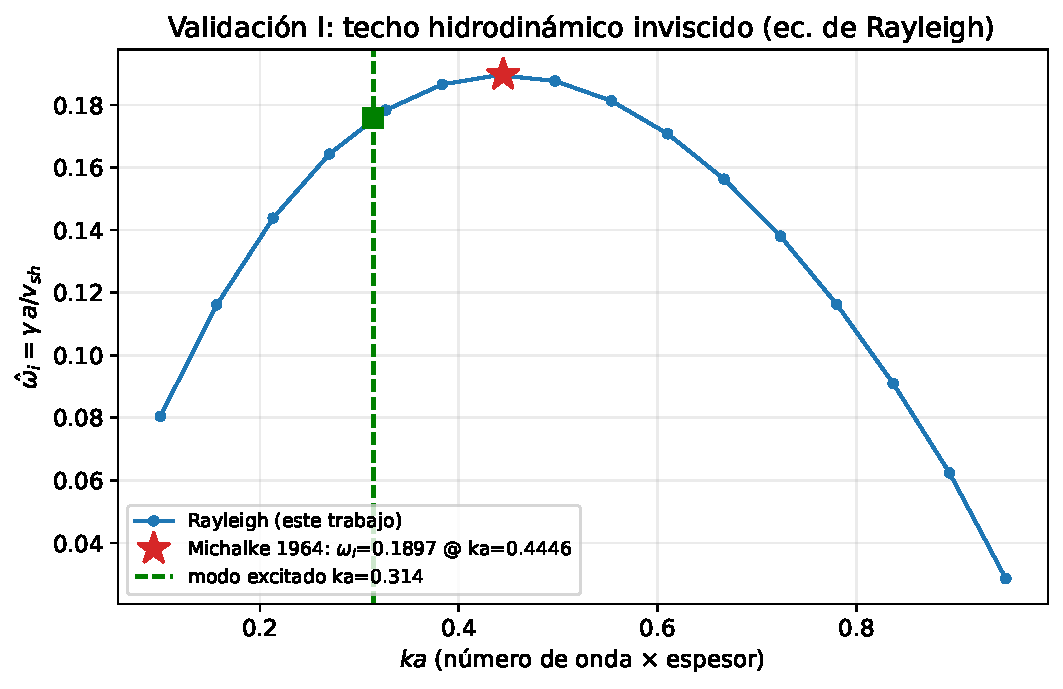
\includegraphics[width=0.92\linewidth]{figures/fig4_michalke.pdf}
  \end{center}
\end{column}
\begin{column}{0.48\textwidth}
  \begin{center}
    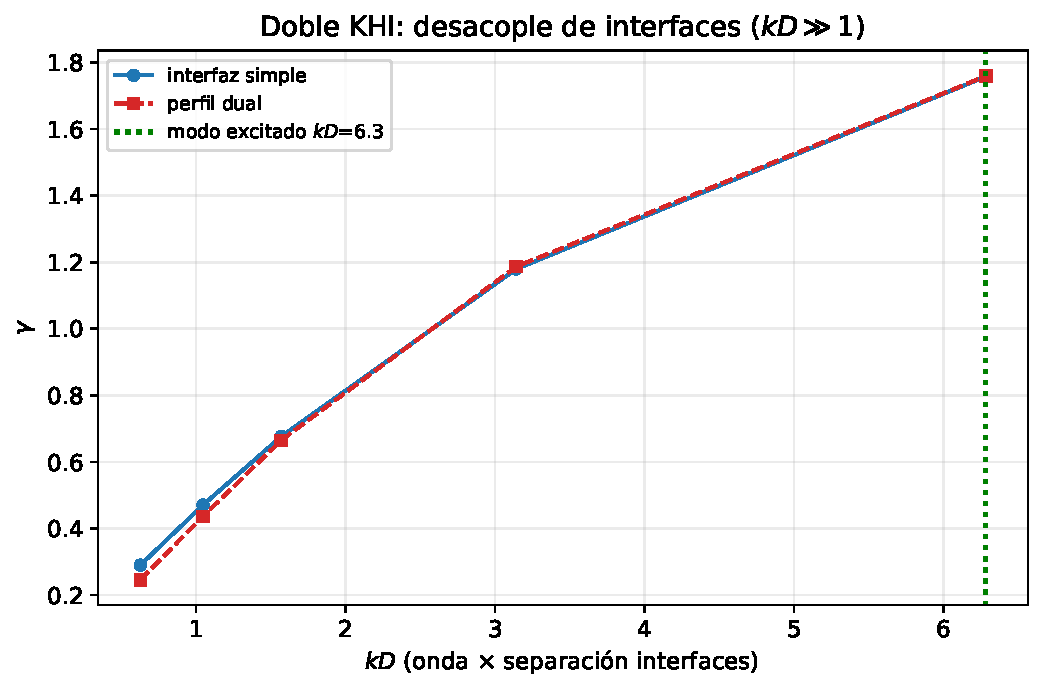
\includegraphics[width=0.92\linewidth]{figures/fig7_dual.pdf}
  \end{center}
\end{column}
\end{columns}
\vspace{0.05cm}
{\scriptsize
\begin{itemize}\setlength\itemsep{1pt}
  \item \textbf{Izq.}: la ecuaci\'on de Rayleigh (perfil $\tanh$) reproduce
        el cl\'asico $\hat\omega_{\max}=0.1897$ en $ka=0.4446$
        \citep{michalke1964}.
  \item \textbf{Der.}: el montaje \emph{doble} no altera el techo ---
        acople $e^{-kD}\approx0.2\%$ en el modo excitado ($kD=2\pi$):
        las dos interfaces crecen desacopladas (diferencia $+0.11\%$).
  \item Doble validaci\'on adicional: l\'imite incompresible de Lees--Lin
        $\to$ Michalke; \emph{vortex sheet} compresible $\to$ umbral de
        Landau $v/c_s=\sqrt2$ \citep{landau1944}.
\end{itemize}}
\end{frame}

%------------------------------------------------------------------------------
% B7 · HLL VS HLLC
%------------------------------------------------------------------------------
\begin{frame}{B7 · ?`Por Qu\'e HLL$+$MP5 y No HLLC?}
\begin{columns}[T]
\begin{column}{0.48\textwidth}
  \begin{block}{El contexto}
    \scriptsize
    El paper del c\'odigo \citep{miranda-aranguren-2018} formula un
    \textbf{HLLC} para RRMHD precisamente porque el HLL \emph{a bajo orden}
    difunde la onda de contacto $\lambda_c=v_x$ --- la que porta la
    cizalla de la KHI.
  \end{block}
  \begin{tcolorbox}[RES={La elecci\'on de este trabajo}]
    \scriptsize
    Para el barrido param\'etrico se us\'o \textbf{HLL $+$ MP5}:
    los propios autores muestran que la agudeza de los estados
    reconstruidos a 5.º orden \emph{compensa} la huella disipativa del HLL,
    igualando en la pr\'actica al HLLC con menor costo, mayor simplicidad
    algebraica y positividad robusta.
  \end{tcolorbox}
\end{column}
\begin{column}{0.48\textwidth}
  \begin{tcolorbox}[EQ={Verificaci\'on emp\'irica en este estudio}]
    \scriptsize
    \begin{itemize}\setlength\itemsep{2pt}
      \item Plateau de $J_{\max}$: la difusividad f\'isica supera el
            truncamiento en toda la zona de transici\'on.
      \item Tasas lineales consistentes al $8\%$ con la teor\'ia
            (imposible si la vorticidad se difundiera artificialmente).
      \item Estratificaci\'on mon\'otona y limpia de las 44 curvas
            $\Omega_{zp}(t)$ con $\sigma$: sin artefactos de esquema.
    \end{itemize}
  \end{tcolorbox}
  \vspace{0.08cm}
  {\scriptsize\color{INF3} La disipaci\'on relevante debe ser la f\'isica
   ($\eta=1/\sigma$); si dominara la num\'erica, $\gamma_{\rm KHI}$ ser\'ia
   insensible a $\sigma$ --- lo contrario de lo observado.}
\end{column}
\end{columns}
\end{frame}

%------------------------------------------------------------------------------
% B8 · ESTADÍSTICA
%------------------------------------------------------------------------------
\begin{frame}{B8 · Estad\'istica del Ajuste Sigmoide}
\begin{columns}[T]
\begin{column}{0.50\textwidth}
  \begin{center}
    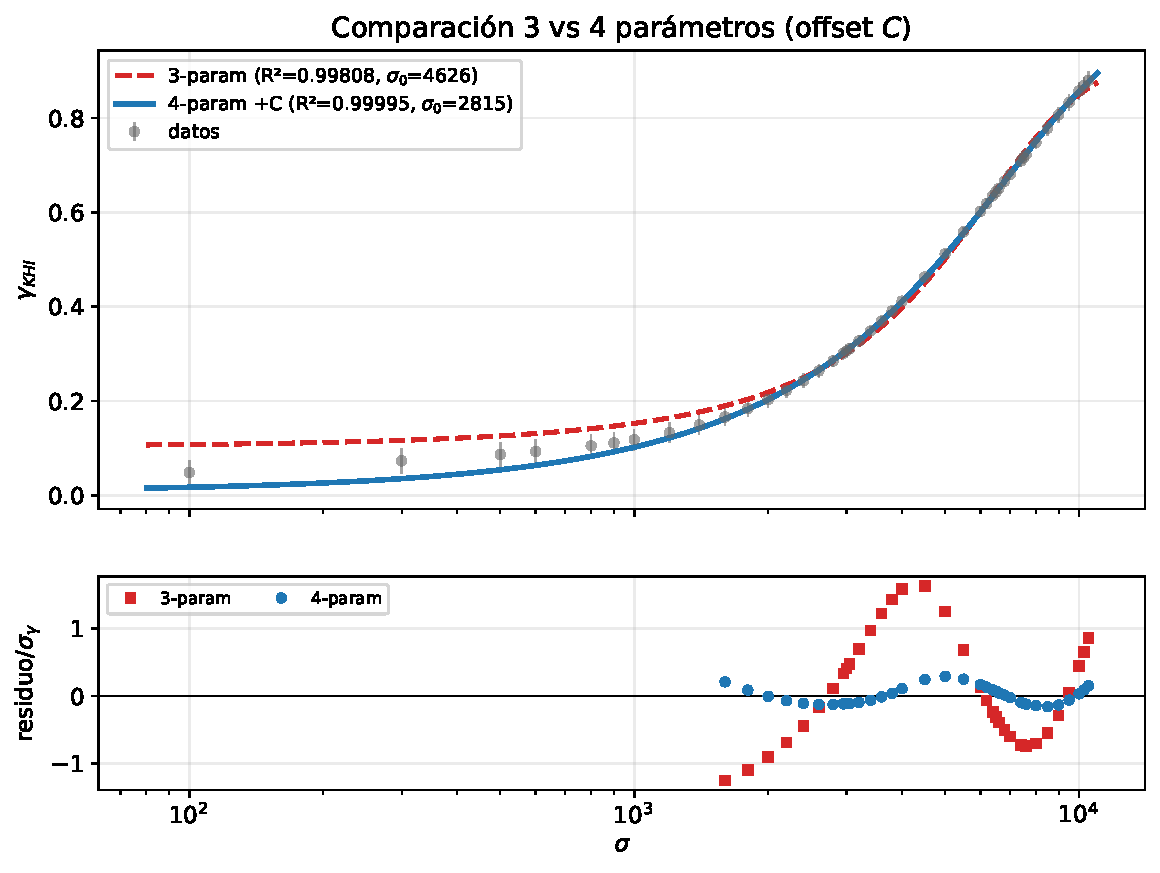
\includegraphics[width=0.95\linewidth]{figures/fig2_3p_vs_4p.pdf}
  \end{center}
\end{column}
\begin{column}{0.46\textwidth}
  \begin{center}
    
\includegraphics[width=0.9\linewidth]{figures/fig10_holdout.pdf}
  \end{center}
\end{column}
\end{columns}
\vspace{0.05cm}
{\scriptsize
\begin{itemize}\setlength\itemsep{1pt}
  \item \textbf{AIC/BIC}: penalizan par\'ametros; $\Delta\mathrm{AIC}=-126$
        (anidado, mismos datos) $\gg10$ $\Rightarrow$ el \emph{offset} no es
        sobreajuste.
  \item \textbf{Test de rachas} (Wald--Wolfowitz): $p<0.05$ $\Rightarrow$
        residuos autocorrelacionados $\Rightarrow$ el error de
        \texttt{curve\_fit} (i.i.d.) subestima.
  \item \textbf{Degeneraci\'on}: $\mathrm{corr}(\gamma_0,C)=-0.997$, pero la
        \textbf{suma} $C+\gamma_0$ es robusta (var\'ia $3.9\%$ entre rangos
        de ajuste): el observable f\'isico es la as\'intota, no cada
        par\'ametro por separado.
  \item $C=-0.45$: par\'ametro de forma con soporte \emph{hold-out};
        no se interpreta como tasa f\'isica en $\sigma\to0$ (zona sin datos).
\end{itemize}}
\end{frame}

%------------------------------------------------------------------------------
% B9 · ESTIMADORES SIGMA CRIT
%------------------------------------------------------------------------------
\begin{frame}{B9 · Los Cuatro Estimadores de $\sigma_{\rm crit}$}
\begin{columns}[T]
\begin{column}{0.55\textwidth}
  \begin{center}
    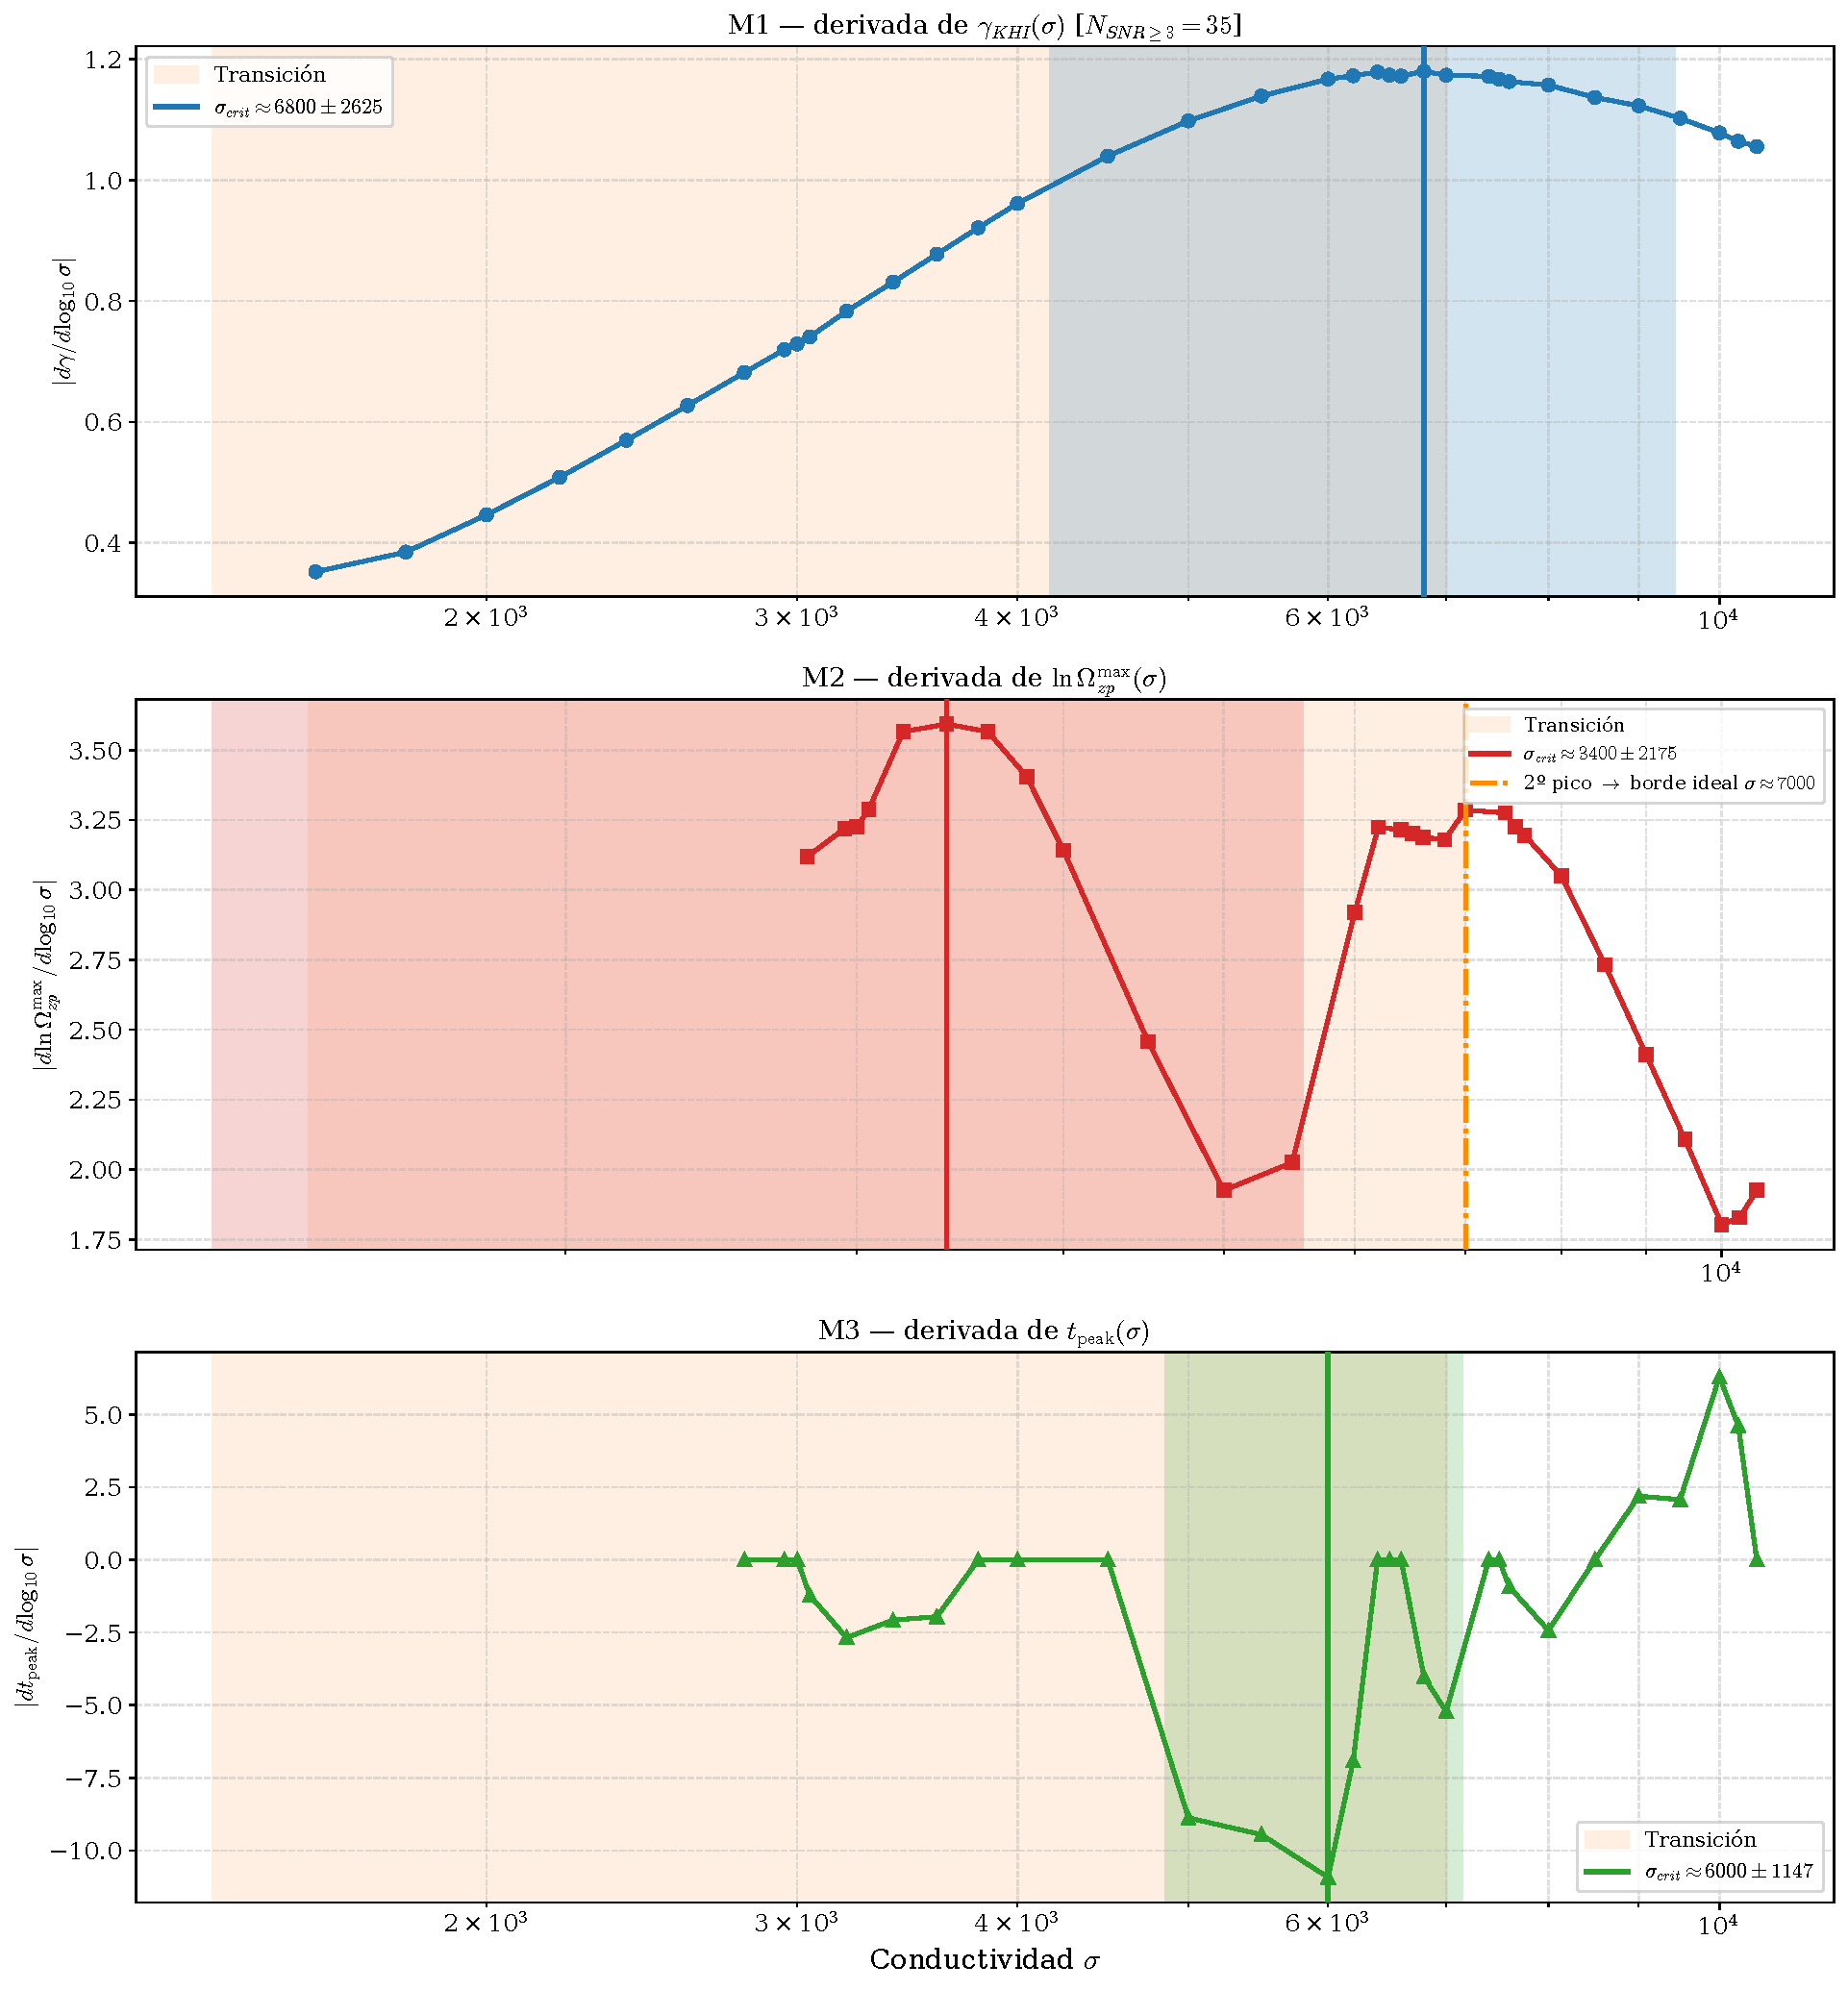
\includegraphics[height=0.74\textheight]{figures/fig_derivadas_scrit.pdf}
  \end{center}
\end{column}
\begin{column}{0.43\textwidth}
  \begin{tcolorbox}[EQ={M\'etodo por inflexi\'on}]
    \scriptsize
    $\sigma_{\rm crit}$ de cada observable $=$ m\'aximo de
    $|d/d\log_{10}\sigma|$; error $=\max(\delta_{\rm jackknife},\,w/2)$.
    \begin{itemize}\setlength\itemsep{1pt}
      \item M4 (sigmoide): $2815\pm123$
      \item M2 ($\Omega^{\max}_{zp}$): $3400\pm2175$
      \item M3 ($t_{\rm peak}$): $6000\pm1147$
      \item M1 ($\gamma$, log): $6800\pm2625$
    \end{itemize}
    Dispersi\'on inter-m\'etodo $\pm1944$ $\Rightarrow$ zona
    $[1400,7000]$, no valor \'unico.
  \end{tcolorbox}
  \begin{center}
    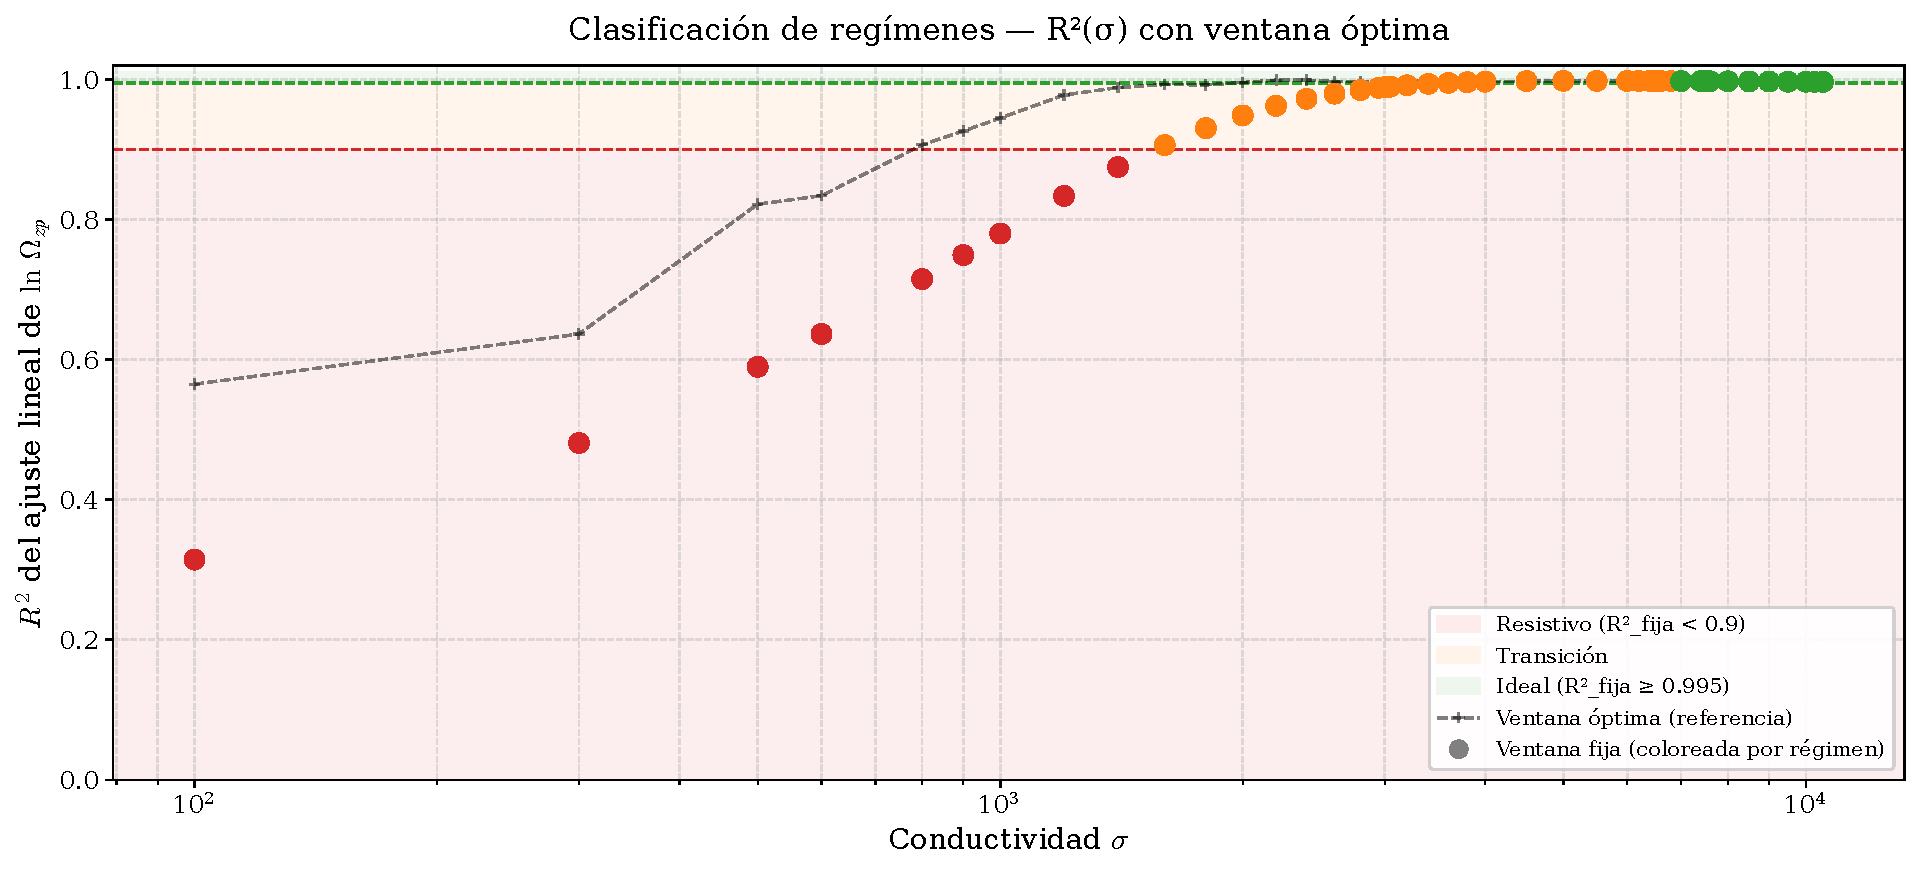
\includegraphics[width=0.85\linewidth]{figures/fig_regimenes.pdf}
  \end{center}
\end{column}
\end{columns}
\end{frame}

%------------------------------------------------------------------------------
% B10 · TABLA CANÓNICA
%------------------------------------------------------------------------------
\begin{frame}{B10 · El Barrido Completo en Conductividad}
\begin{columns}[T]
\begin{column}{0.58\textwidth}
  \begin{center}
    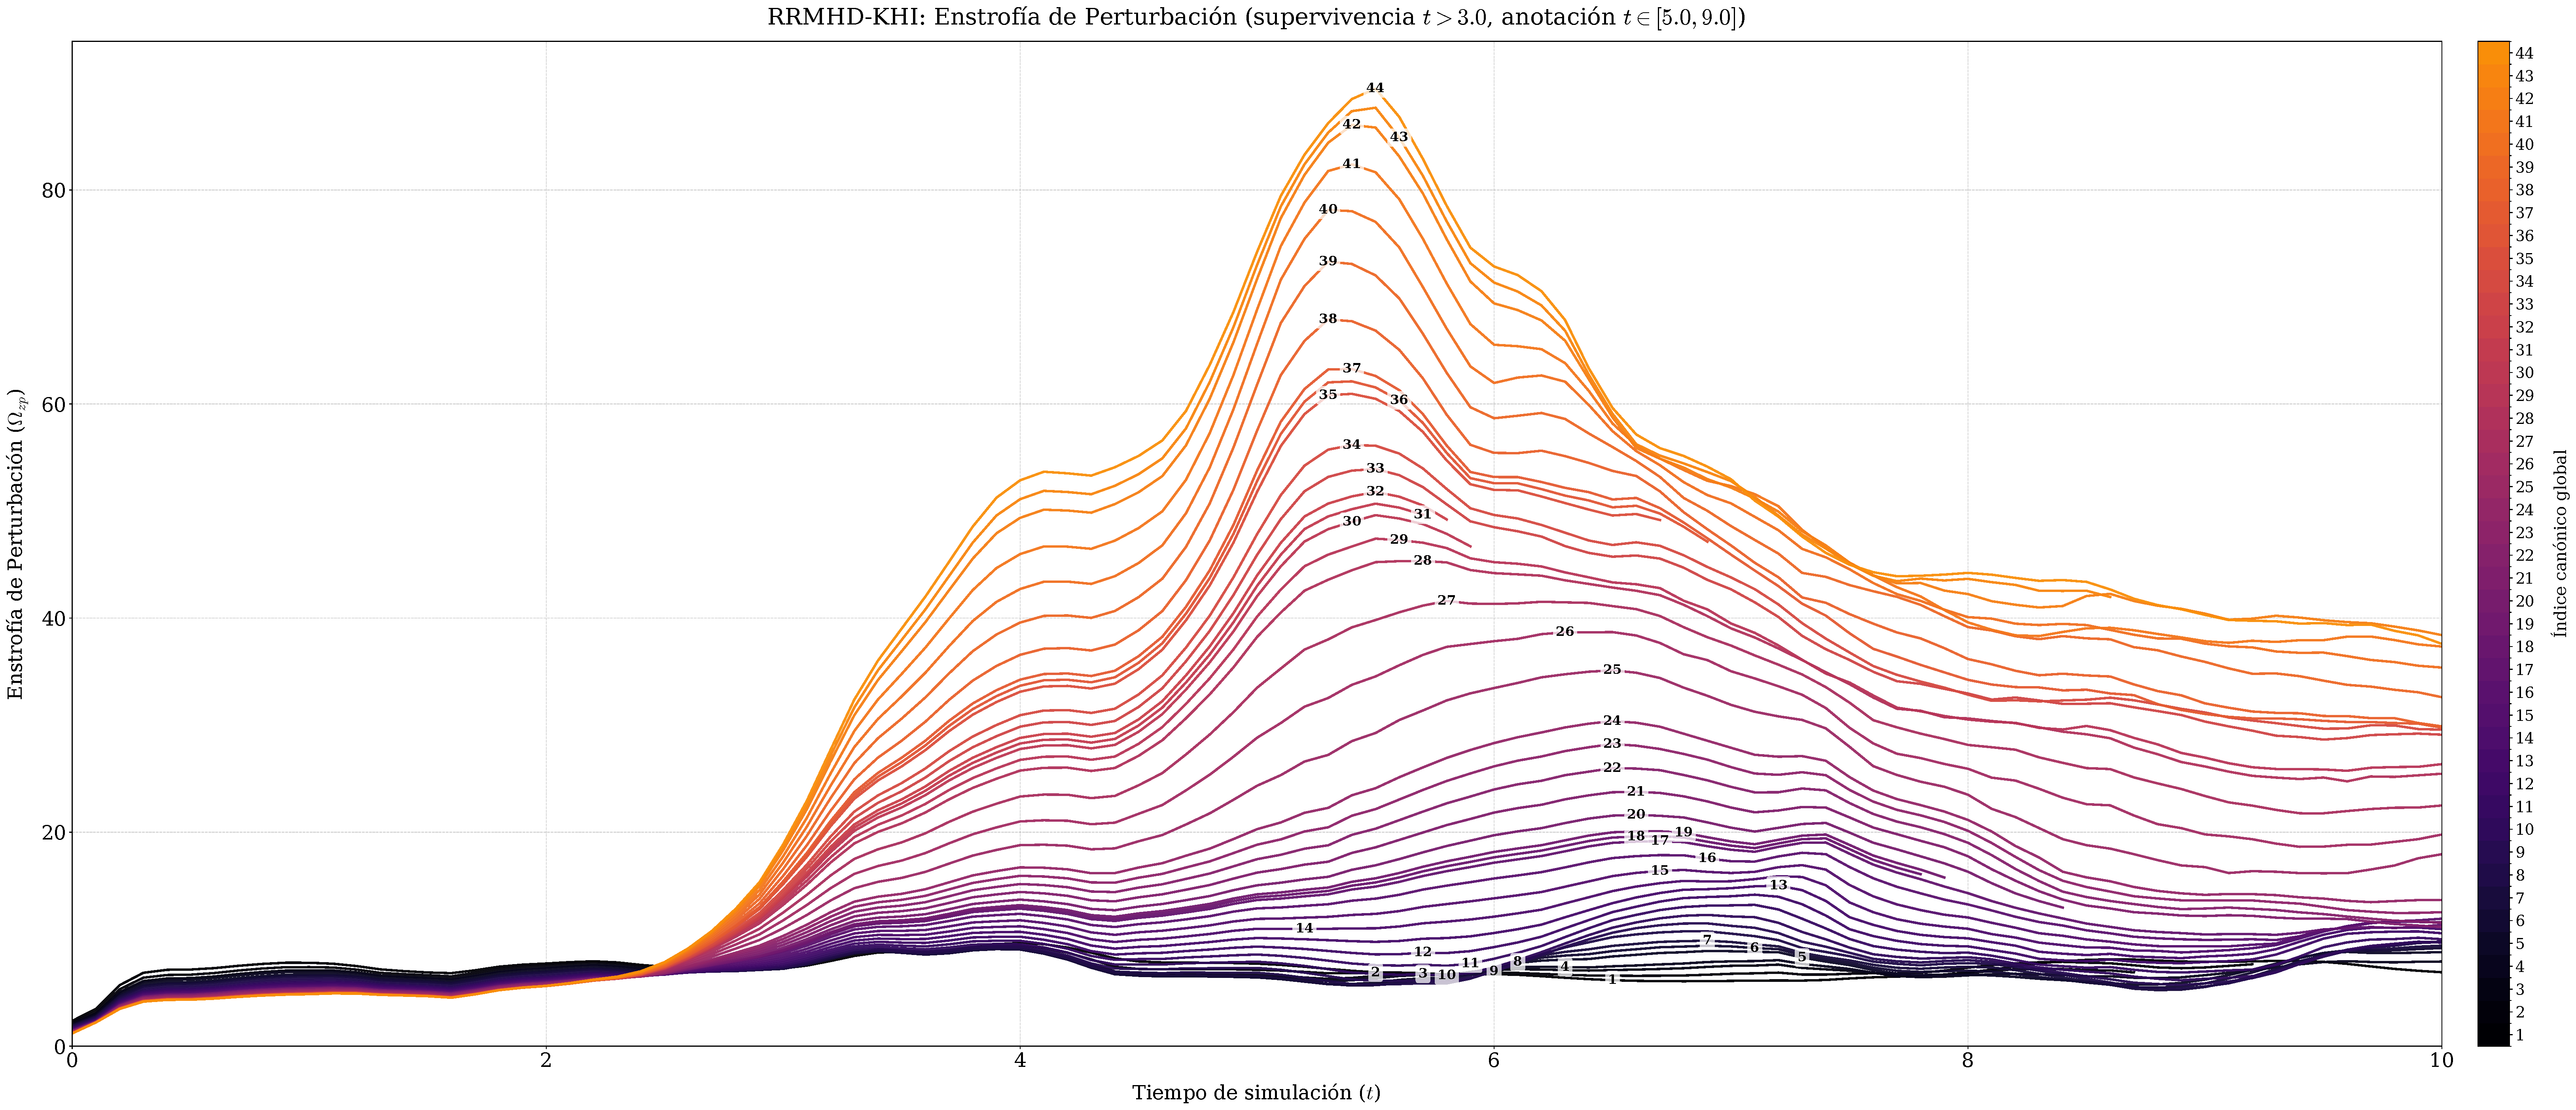
\includegraphics[width=\linewidth]{figures/fig_ultrawide_omega_zp.pdf}\\[2pt]
    {\tiny\color{INF3} $\Omega_{zp}(t)$, 44 simulaciones; color $=$ \'indice
     can\'onico (negro$\to$naranja $=$ $\sigma$ creciente).}
  \end{center}
\end{column}
\begin{column}{0.40\textwidth}
  \begin{tcolorbox}[EQ={Subconjuntos de an\'alisis}]
    \scriptsize
    \begin{itemize}\setlength\itemsep{2pt}
      \item $\sigma\in[100,10\,500]$, $N=44$ (\'indice can\'onico $j$).
      \item Ajuste de $\gamma_{\rm KHI}$ y $\sigma_{\rm crit}$:
            $N=35$ ($\sigma\ge1600$, $R^2\ge0.90$, SNR $\ge3$).
      \item Ajustes de pico ($\Omega^{\max}$, $t_{\rm peak}$):
            $N=29$ ($\sigma\ge2800$, pico identificable dentro del
            horizonte temporal).
    \end{itemize}
    Los dos subconjuntos difieren porque la pendiente lineal es medible
    antes ($\sigma\ge1600$) que el pico ($\sigma\ge2800$).
  \end{tcolorbox}
\end{column}
\end{columns}
\end{frame}

%------------------------------------------------------------------------------
% B11 · VLASOV → FLUIDO
%------------------------------------------------------------------------------
\begin{frame}{B11 · Del Espacio de Fase al Fluido: Fundamento del Continuo}
\begin{columns}[T]
\begin{column}{0.50\textwidth}
  \begin{tcolorbox}[EQ={La jerarqu\'ia de momentos}]
    \scriptsize
    Liouville $\Rightarrow$ la densidad $f(\mathbf x,\mathbf p,t)$ se
    conserva a lo largo del flujo hamiltoniano; con colisiones:
    Boltzmann--Vlasov. Los \textbf{momentos} de $f$ (densidad, momento,
    energ\'ia) generan la jerarqu\'ia fluida; la RRMHD la \textbf{trunca}
    asumiendo:
    \begin{itemize}\setlength\itemsep{1pt}
      \item equilibrio termodin\'amico local (colisionalidad alta),
      \item cierre EoS politr\'opico ($\Gamma=4/3$),
      \item transporte reducido a UNA constante: $\sigma$.
    \end{itemize}
  \end{tcolorbox}
\end{column}
\begin{column}{0.46\textwidth}
  \begin{tcolorbox}[WRN={D\'onde colapsa la aproximaci\'on}]
    \scriptsize
    \begin{itemize}\setlength\itemsep{2pt}
      \item Plasma diluido / campo extremo: la conducci\'on se vuelve
            anisotr\'opica ($\sigma$ tensorial, Hall).
      \item Escalas $\lesssim$ girorradio: din\'amica cin\'etica
            (PIC / h\'ibridos fluido-cin\'eticos).
      \item En este trabajo la escala disipativa resuelta es la capa
            resistiva $\delta\sim S^{-1/2}$ --- \emph{macrosc\'opica} ---
            y all\'i el cierre unifluido es consistente.
    \end{itemize}
  \end{tcolorbox}
  \vspace{0.08cm}
  {\scriptsize\color{INF3} La simulaci\'on es un puente entre la teor\'ia de
   campos y la fenomenolog\'ia observable; sus l\'imites de validez son
   parte del resultado, no una debilidad ocultable.}
\end{column}
\end{columns}
\end{frame}

%------------------------------------------------------------------------------
% B12 · RECURSOS COMPUTACIONALES
%------------------------------------------------------------------------------
\begin{frame}{B12 · Recursos Computacionales y Flujo de Trabajo}
\begin{columns}[T]
\begin{column}{0.48\textwidth}
  \begin{tcolorbox}[EQ={El c\'odigo}]
    \scriptsize
    \begin{itemize}\setlength\itemsep{2pt}
      \item \texttt{Cueva} (\textit{Computing Unit for Environments in
            Astrophysics}): Fortran 95 modular; RRMHD en la formulaci\'on
            de \citet{komissarov-2007}.
      \item M\'odulos clave: variables conservadas, reconstrucci\'on MP5,
            flujos HLL, paso IMEX, recuperaci\'on de primitivas
            (Ferrari--Cardano).
      \item Desarrollado por el director
            \citep{miranda-aranguren-2014,miranda-aranguren-2018}.
    \end{itemize}
  \end{tcolorbox}
\end{column}
\begin{column}{0.48\textwidth}
  \begin{tcolorbox}[RES={La campa\~na}]
    \scriptsize
    \begin{itemize}\setlength\itemsep{2pt}
      \item $\approx30\,000$ horas-n\'ucleo en el servidor facilitado por
            la Universidad Distrital.
      \item $44+18$ simulaciones; snapshots $+$ series temporales de
            diagn\'osticos.
      \item An\'alisis en Python (NumPy/SciPy/Matplotlib):
            regresiones, ajuste no lineal, autovalores de la teor\'ia
            lineal (Rayleigh / Lees--Lin), validaci\'on estad\'istica.
      \item Repositorio con visualizaciones:
            \texttt{github.com/Sebrodriguezg/KHI}.
    \end{itemize}
  \end{tcolorbox}
\end{column}
\end{columns}
\end{frame}

%------------------------------------------------------------------------------
% B13 · FIGURAS ADICIONALES
%------------------------------------------------------------------------------
\begin{frame}{B13 · Estructuras Secundarias y Campa\~na C}
\begin{columns}[T]
\begin{column}{0.48\textwidth}
  \begin{center}
    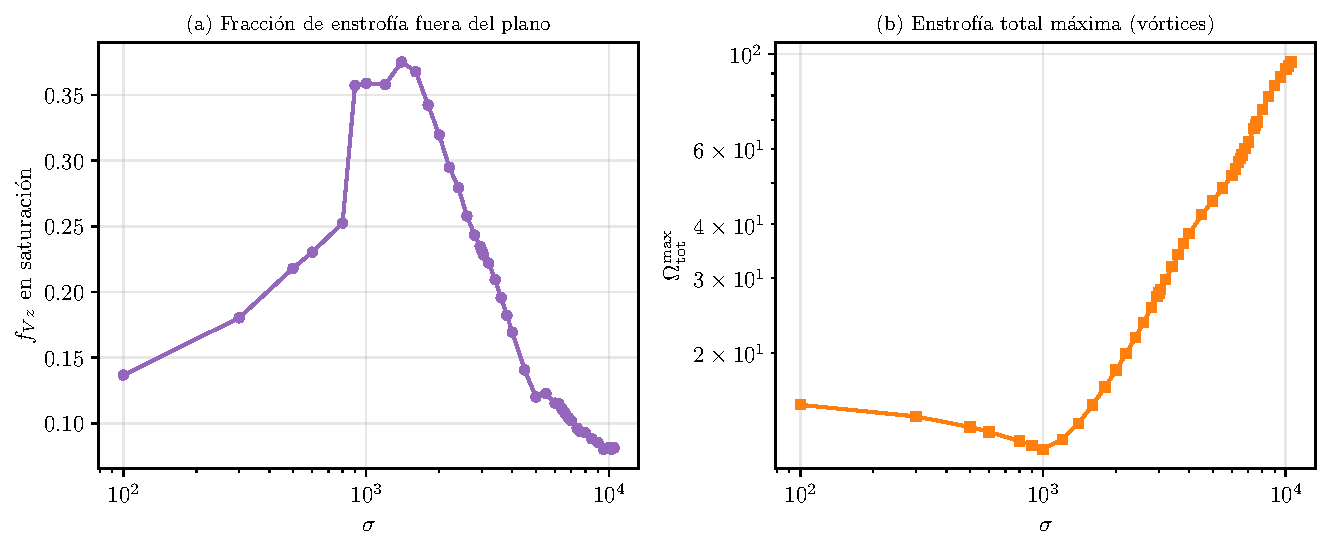
\includegraphics[width=\linewidth]{figures/fig_global_estructuras.pdf}\\[1pt]
    {\tiny\color{INF3} $f_{Vz}$ en saturaci\'on: m\'aximo en la transici\'on
     ($\sigma\approx1400$), suprimido en el ideal.}
  \end{center}
\end{column}
\begin{column}{0.48\textwidth}
  \begin{center}
    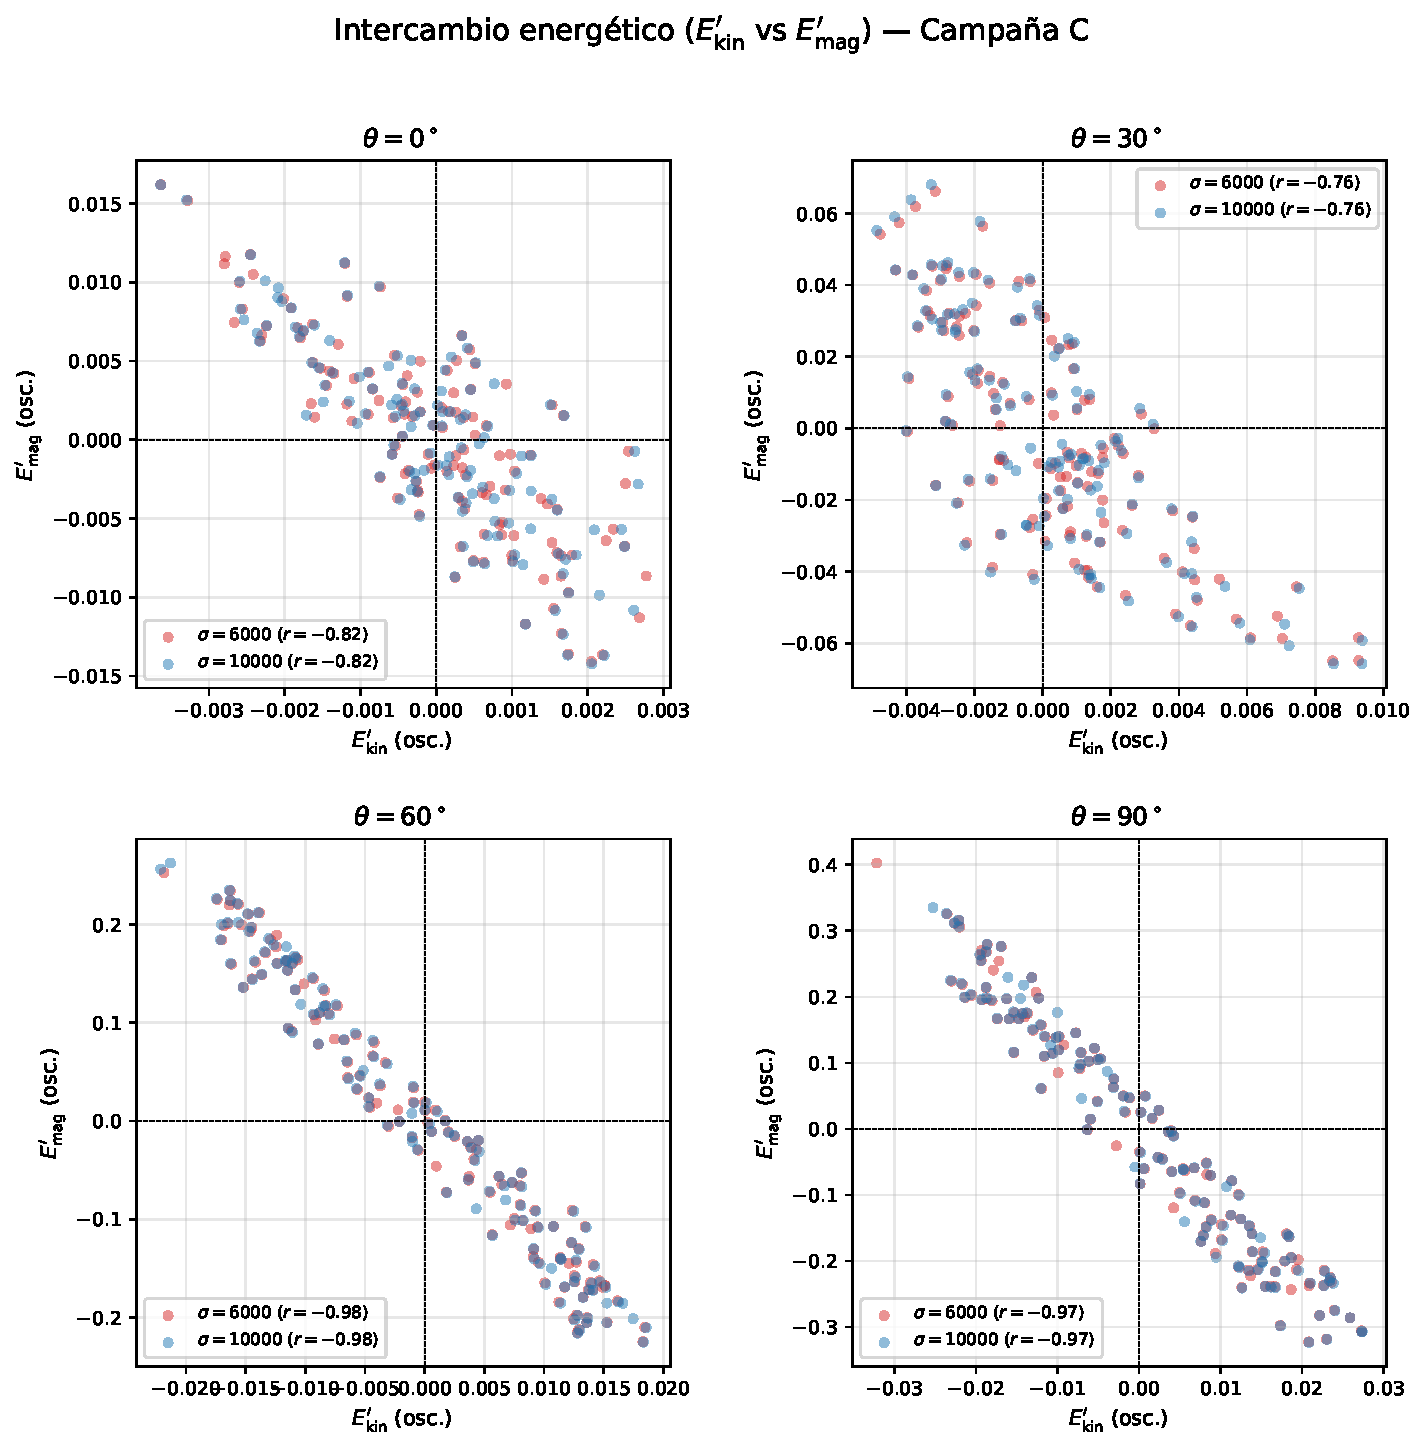
\includegraphics[width=\linewidth]{figures/fig_campC_ekin_emag_scatter.pdf}\\[1pt]
    {\tiny\color{INF3} Campa\~na C (sin tensi\'on): anti-correlaci\'on
     cin\'etico--magn\'etica hasta $r\approx-0.98$.}
  \end{center}
\end{column}
\end{columns}
\end{frame}

%------------------------------------------------------------------------------
% B14 · MAPAS DE DENSIDAD CAMPAÑAS
%------------------------------------------------------------------------------
\begin{frame}{B14 · Mapas de Densidad de las Campa\~nas Magn\'eticas}
\begin{columns}[T]
\begin{column}{0.48\textwidth}
  \begin{center}
    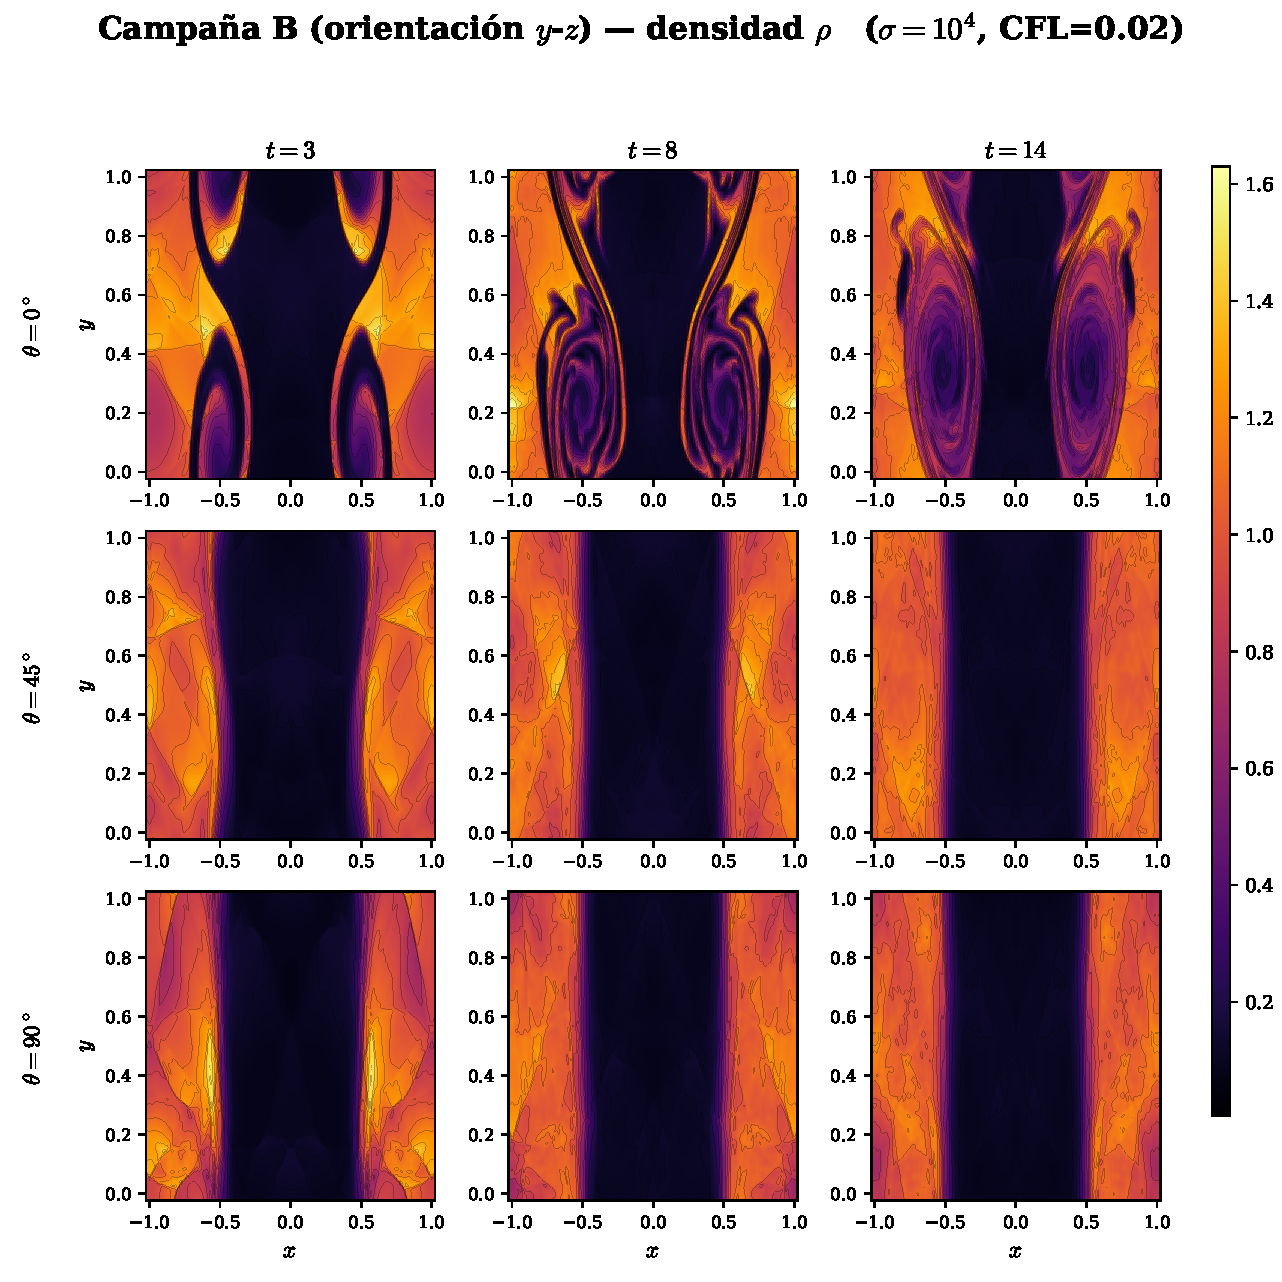
\includegraphics[width=\linewidth]{figures/fig_campB_rho_collage.pdf}\\[1pt]
    {\tiny\color{INF3} Campa\~na B: al crecer $\theta$ (tensi\'on),
     el enrollamiento se suprime.}
  \end{center}
\end{column}
\begin{column}{0.48\textwidth}
  \begin{center}
    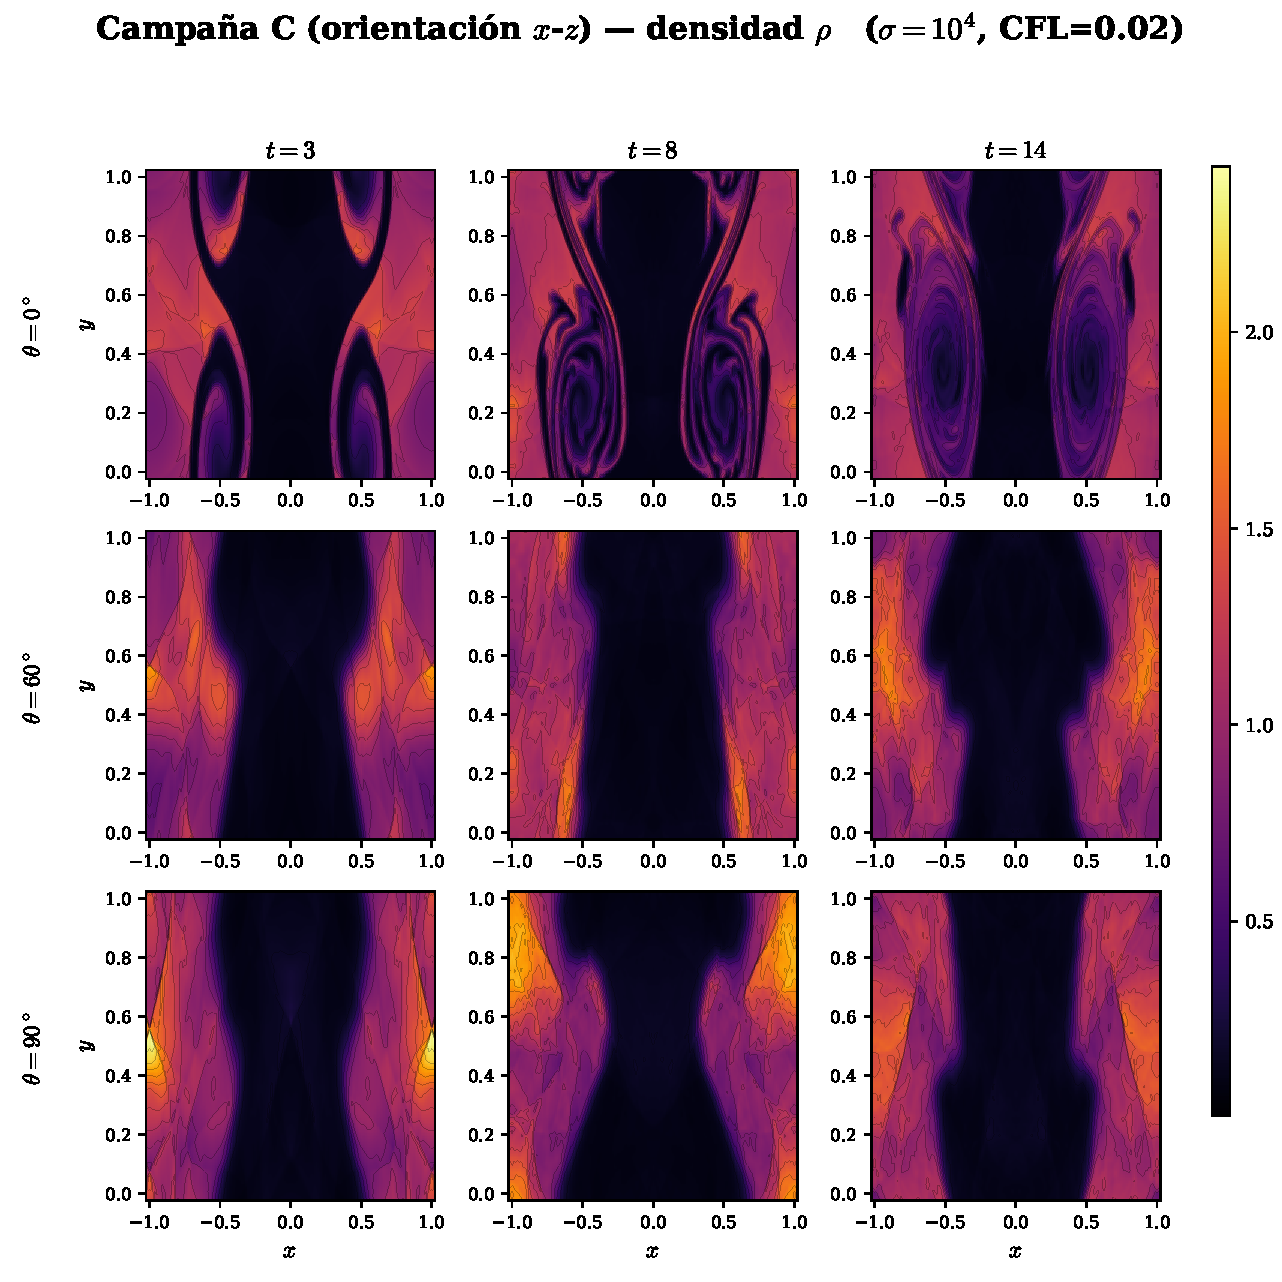
\includegraphics[width=\linewidth]{figures/fig_campC_rho_collage.pdf}\\[1pt]
    {\tiny\color{INF3} Campa\~na C: sin tensi\'on, crecimiento sin fase
     lineal limpia y mezcla difusa.}
  \end{center}
\end{column}
\end{columns}
\end{frame}

%------------------------------------------------------------------------------
% B15 · TABLERO DINÁMICO DE LA CAMPAÑA B (frame del video)
%------------------------------------------------------------------------------
\begin{frame}{B15 · Tablero Din\'amico de la Campa\~na B ($\sigma=6000$ vs $10^4$)}
\begin{center}
  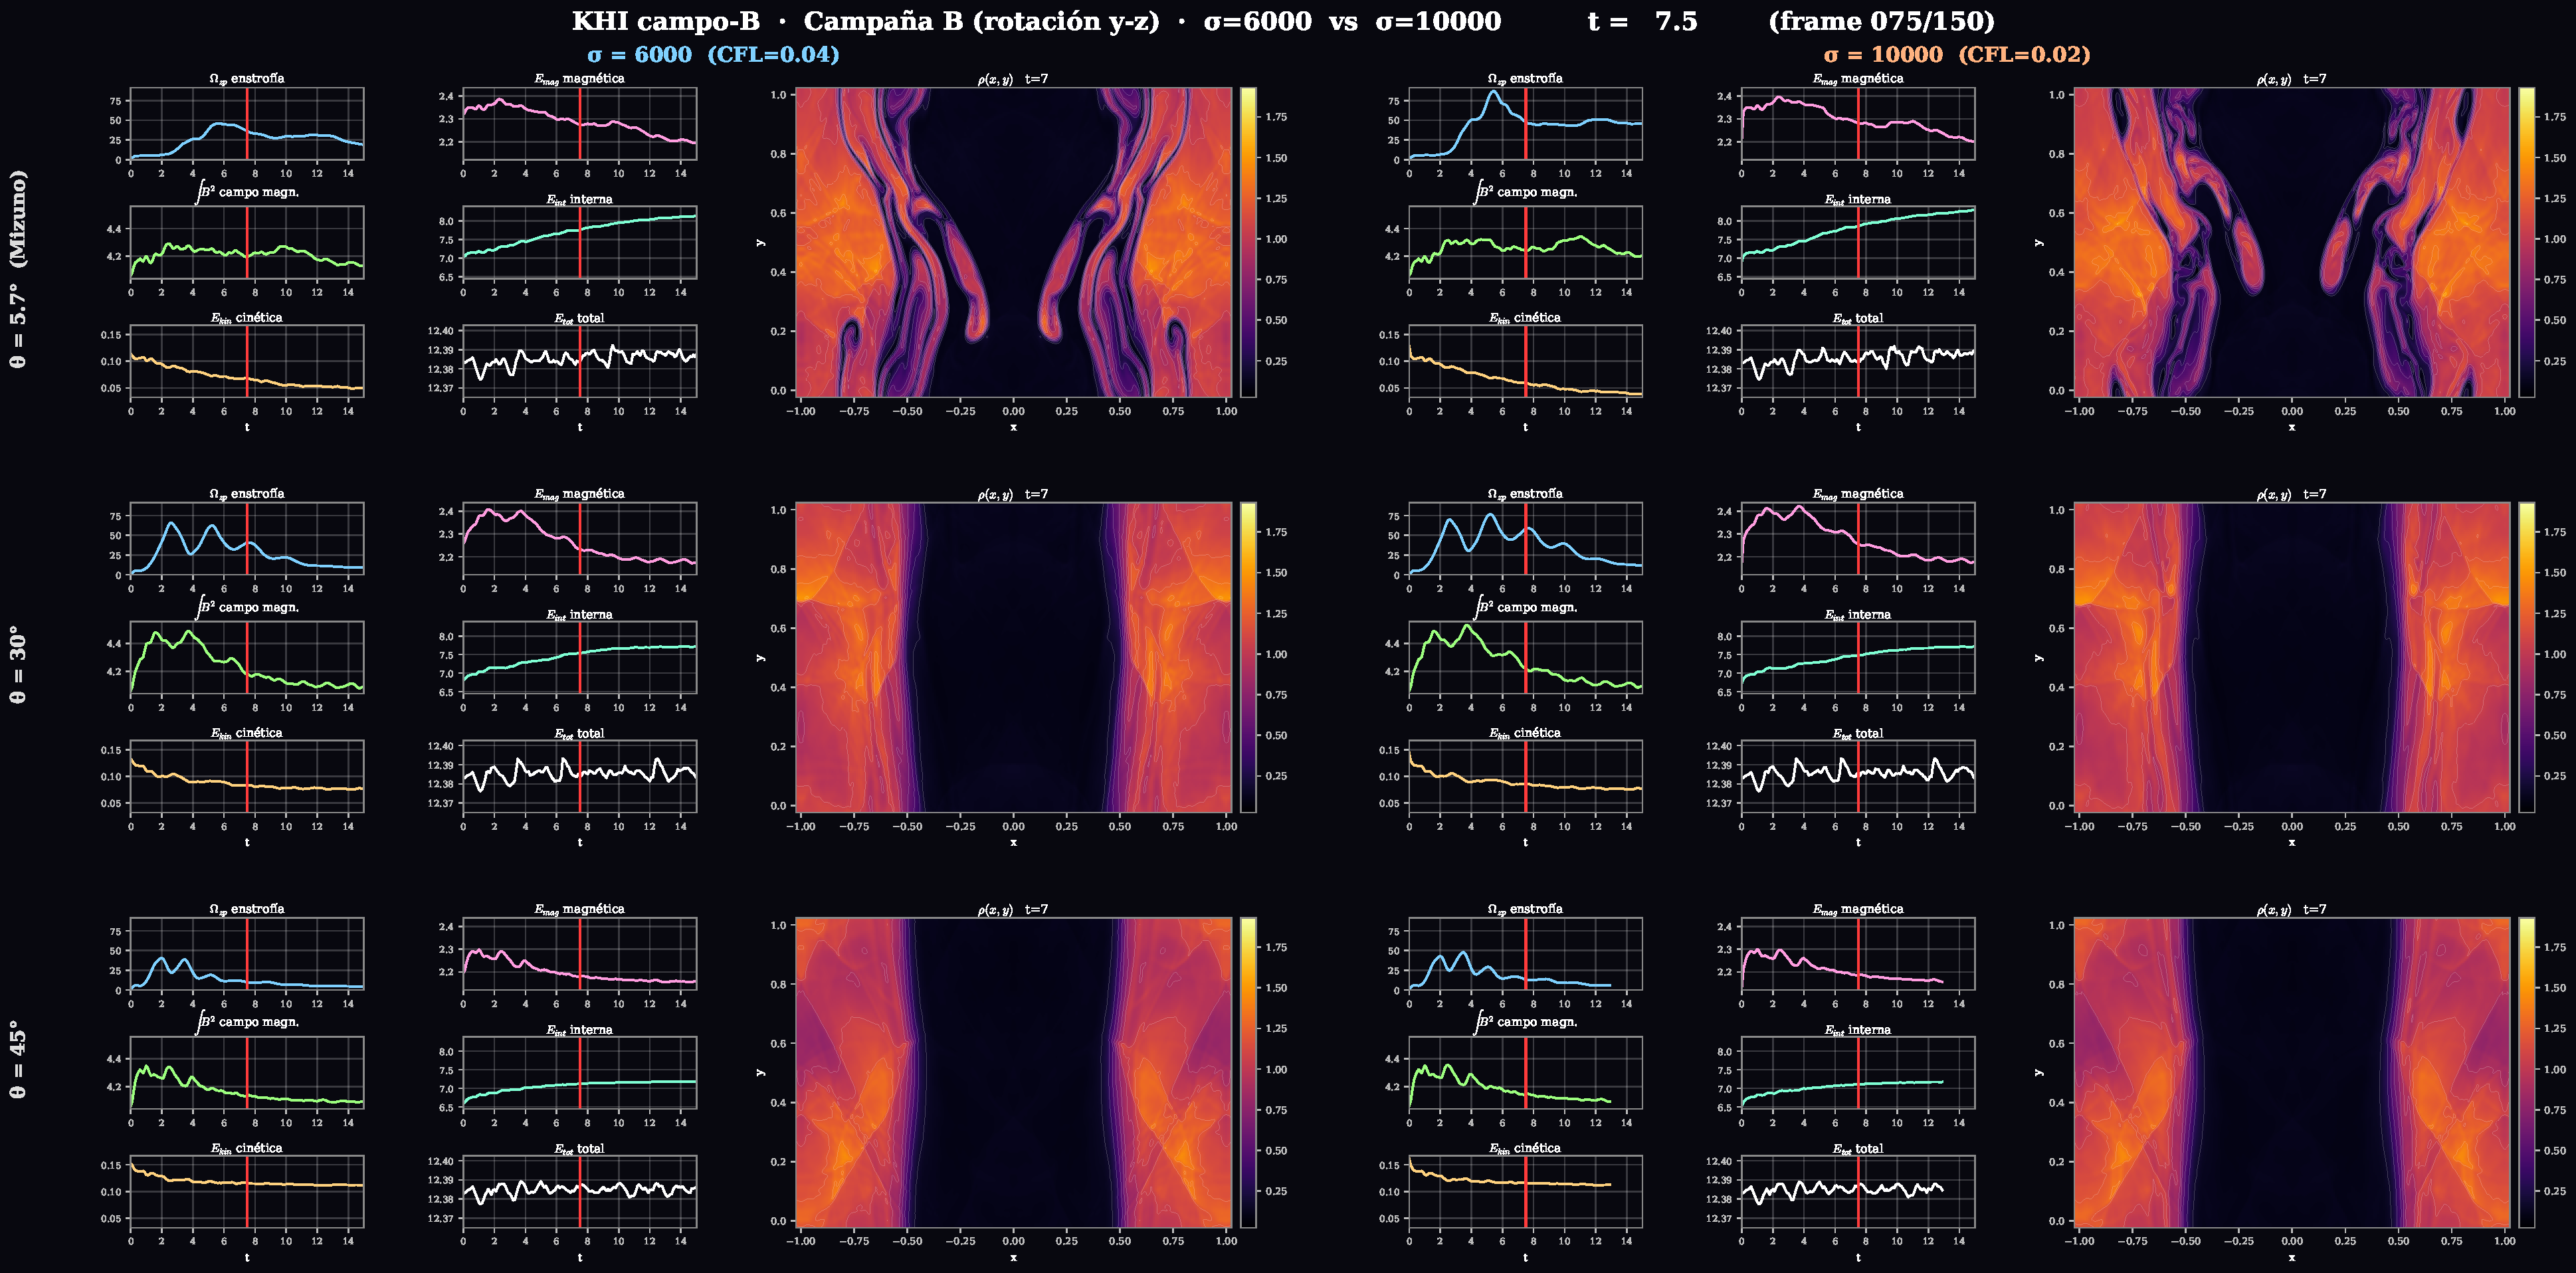
\includegraphics[width=0.84\textwidth]{figures/campB_dashboard_t7p5.pdf}\\[2pt]
  {\tiny\color{INF3} Fotograma $t=7.5$ del tablero animado (150 frames):
   filas $=\theta$; por $\sigma$: 6 diagn\'osticos globales $+$ mapa
   $\rho(x,y)$ sincronizados (cursor rojo). Hay video para la discusi\'on.}
\end{center}
\end{frame}

\end{document}
